\documentclass[12pt]{report}

\usepackage{paquetes_todos}

\usepackage[showboxes]{textpos}

\begin{document}
% Portada
\title{Estudios de simulación en la búsqueda de nuevos bosones ligeros durante la fase de alta luminosidad del experimento CMS del CERN}
\author{Francisco Martínez Sánchez}
\prevdegrees{MBs. Physics}
%\prevdegrees{Grados previos}
\institute{UNISON}
\department{Departamento de Investigación en Física}
\degree{Maestro en Ciencias}
\supervisor{Dr. Alfredo Castañeda}
\city{Hermosillo, Sonora, México}
\degreemonth{Julio}
\degreeyear{2020}
\maketitle
%\begin{acknowledgements}\thispagestyle{empty}
%xxxx
%\end{acknowledgements}
%
\newcommand{\fermion}{\href{https://es.wikipedia.org/wiki/Fermi\%C3\%B3n}{fermion}}
\newcommand{\fermiones}{\href{https://es.wikipedia.org/wiki/Fermi\%C3\%B3n}{fermiones}}

\newcommand{\boson}{\href{https://es.wikipedia.org/wiki/Bos\%C3\%B3n}{boson}}
\newcommand{\bosones}{\href{https://es.wikipedia.org/wiki/Bos\%C3\%B3n}{bosones}}

\newcommand{\fermidirac}{\href{https://es.wikipedia.org/wiki/Estad\%C3\%ADstica_de_Fermi-Dirac}{estadística de Fermi-Dirac}}

\newcommand{\boseeinstein}{\href{https://es.wikipedia.org/wiki/Estad\%C3\%ADstica_de_Bose-Einstein}{estadística de Bose-Einstein}}


\newcommand{\pauli}{\href{https://es.wikipedia.org/wiki/Principio_de_exclusi\%C3\%B3n_de_Pauli}{principio de exclusión de Pauli}}

\newcommand{\quark}{\href{https://es.wikipedia.org/wiki/Quark}{quark}}
\newcommand{\Quark}{\href{https://es.wikipedia.org/wiki/Quark}{Quark}}
\newcommand{\Quarks}{\href{https://es.wikipedia.org/wiki/Quark}{Quark}}
\newcommand{\quarks}{\href{https://es.wikipedia.org/wiki/Quark}{quarks}}

\newcommand{\lepton}{\href{https://es.wikipedia.org/wiki/Lept\%C3\%B3n}{lepton}}
\newcommand{\leptones}{\href{https://es.wikipedia.org/wiki/Lept\%C3\%B3n}{leptones}}
\newcommand{\Leptones}{\href{https://es.wikipedia.org/wiki/Lept\%C3\%B3n}{leptones}}

\newcommand{\hadron}{\href{https://es.wikipedia.org/wiki/Hadr\%C3\%B3n}{hadron}}
\newcommand{\hadrones}{\href{https://es.wikipedia.org/wiki/Hadr\%C3\%B3n}{hadrones}}

\newcommand{\matterspectrum}{\href{https://en.wikipedia.org/wiki/Matter_power_spectrum}{Harrison--Zeldovich}}


\newcommand{\Axion}{\href{https://en.wikipedia.org/wiki/Axion}{Axion}}
\newcommand{\axion}{\href{https://en.wikipedia.org/wiki/Axion}{axion}}
\newcommand{\Axiones}{\href{https://en.wikipedia.org/wiki/Axion}{Axiones}}
\newcommand{\axiones}{\href{https://en.wikipedia.org/wiki/Axion}{axiones}}



\newcommand{\neutralinos}{\href{https://en.wikipedia.org/wiki/Neutralino}{neutralinos}}
\newcommand{\neutralino}{\href{https://en.wikipedia.org/wiki/Neutralino}{neutralino}}

\newcommand{\WIMP}{\href{https://en.wikipedia.org/wiki/Weakly_interacting_massive_particles}{\textbf{WIMP}}}
\newcommand{\WIMPs}{\href{https://en.wikipedia.org/wiki/Weakly_interacting_massive_particles}{\textbf{WIMPs}}}

\newcommand{\LSP}{\href{https://en.wikipedia.org/wiki/Lightest_supersymmetric_particle}{\textbf{LSP}}}


%%%%% Siglas %%%%


\newcommand{\CMB}{\href{https://en.wikipedia.org/wiki/Cosmic_microwave_background}{\textbf{CMB}}}

\newcommand{\LHC}{\href{https://es.wikipedia.org/wiki/Gran_colisionador_de_hadrones}{\textbf{LHC}}}

\newcommand{\CERN}{\href{https://es.wikipedia.org/wiki/Organizaci\%C3\%B3n_Europea_para_la_Investigaci\%C3\%B3n_Nuclear}{\textbf{CERN}}}

\newcommand{\CMS}{\href{https://en.wikipedia.org/wiki/Compact_Muon_Solenoid}{\textbf{CMS}}}

\newcommand{\ROOT}{\href{https://en.wikipedia.org/wiki/ROOT}{\textbf{ROOT}}}

\newcommand{\MSSM}{\href{https://en.wikipedia.org/wiki/Minimal_Supersymmetric_Standard_Model}{\textbf{MSSM}}}

\newcommand{\WMAP}{\href{https://en.wikipedia.org/wiki/Wilkinson_Microwave_Anisotropy_Probe}{\textbf{WMAP}}}

\newcommand{\ME}{\href{https://es.wikipedia.org/wiki/Modelo_est\%C3\%A1ndar_de_la_f\%C3\%ADsica_de_part\%C3\%ADculas}{\textbf{SM}}}

\newcommand{\MC}{\href{https://en.wikipedia.org/wiki/Monte_Carlo}{\textbf{MC}}}


\newcommand{\LG}{\href{https://es.wikipedia.org/wiki/Fantasma_de_Fadd\%C3\%A9yev-Popov}{lagrangiano fantasma}}

\newcommand{\EW}{\href{https://es.wikipedia.org/wiki/Modelo_electrod\%C3\%A9bil}{\textbf{EW}}}

\newcommand{\QCD}{\href{https://es.wikipedia.org/wiki/Cromodin\%C3\%A1mica_cu\%C3\%A1ntica}{\textbf{QCD}}}

\newcommand{\SUSY}{\href{https://en.wikipedia.org/wiki/Supersymmetry}{\textbf{SUSY}}}





\begin{resumen}\thispagestyle{empty}
En el presente trabajo se analiza el decaimiento $h \rightarrow 2n_1 \rightarrow 2n_D + 2\gamma_D \rightarrow 2n_D + 4\mu$ correspondiente al modelo \textbf{Dark-}\SUSY ~o \MSSM\textbf{D}~ el cual predice la existencia del fotón oscuro ($\gamma_{D}$), candidato a explicar la naturaleza de la materia oscura. El análisis se realiza usando muestras de simulación generadas con paquetes especializados (\textsfSmall{Madgraph5}, \textsfSmall{Pythia8} y \textsfSmall{Delphes}) y considerando variaciones en los par\'ametros del modelo $m_{n_1}$, $m_{n_D}$ y $m_{\gamma_D}$ y tiempo de vida del fotón oscuro $c\tau_{\gamma_D}$, la parte experimental considera la reconstrucción de la señal con la configuración actual del detector \CMS~ (Run-2) y las condiciones futuras en la etapa de alta luminosidad.
Se comprobó que la configuración del detector \CMS~ correspondiente a Run-2 permite reconstruir hasta un máximo del $\sim 28.7\%$ de los fotones oscuros $\gamma_D$ predichos por la teoría, por otro lado en la configuración de Alta Luminosidad se podrá hasta un $\sim 42.6\%$. Además, con la actualización se disminuye el error en las distribuciones de masa invariante del fotón oscuro de $\sim 12\% - 28\%$. La implementación de dos métodos de identificación de fotones oscuros como resultado de emparejamiento en di-muones, uno basado en redes neuronales permitiendo reconstruir un mínimo de $92\%$ del total teórico posible y otro en un método iterativo de comparación con minimización de las diferencias de las masas invariantes reconstruidas permitiendo un máximo de $\sim 44\%$.



%las distribuciones de las propiedades del fotón oscuro y de los muones, se muestra un aumento del dominio de los valores de la pseudorapidez desde $|\eta|\lesssim 2.4$ a $|\eta|\lesssim 4$ y del momento transversal $P_T\lesssim 10$ GeV a $P_T\lesssim.1$ GeV con la actualización del detector, resultando en un aumento de reconstrucción de un mínimo de $36\%$ muones. 


\end{resumen}
\begin{abstract}\thispagestyle{empty}%\addcontentsline{toc}{chapter}{Abstract}
This work analyzes the decay $ h \rightarrow 2n_1 \rightarrow 2n_D + 2 \gamma_D \rightarrow 2n_D + 4 \mu$ corresponding to the model \textbf{Dark-}\SUSY ~ o \MSSM\textbf{D} which predicts the existence of the dark photon ($\gamma_{D}$), candidate to explain the nature of dark matter. The analysis is performed using simulation samples generated with specialized packages (\textsfSmall{Madgraph5}, \textsfSmall{Pythia8} and \textsfSmall{Delphes}) and considering variations in the parameters of the model $m_{n_1} $, $m_{n_D} $ and $m_{\gamma_D} $ and lifetime of the dark photon $c\tau_{\gamma_D}$, the experimental considers the reconstruction of the signal with the current configuration of the detector \CMS ~ (Run-2) and the future conditions in the high-light stage. It was verified that the detector configuration \CMS ~ corresponding to Run-2 allows to reconstruct up to a maximum of $\sim 28.7 \% $ of the dark photons $\gamma_D$ predicted by the theory, on the other hand in the High Luminosity configuration up to $\sim 42.6 \% $ will be allowed. In addition, the update reduces the error in the invariant mass distributions of the dark photon by $\sim 12 \% - 28 \%$. The implementation of two methods of identifying dark photons as a result of pairing in di-muons, one based on neural networks allowing the reconstruction of a minimum of $92 \%$ of the possible theoretical total and the other in an iterative method of comparison with minimization of differences of the reconstructed invariant masses allowing a maximum of $\sim 44 \%$.\\[1cm]
%\textbf{Keywords:} Supersymmetry,\MSSM, \CMS, \CERN, \textbf{RNA}, 
\end{abstract}

\setcounter{page}{1}
\tableofcontents
\clearpage
\listoftables
\addcontentsline{toc}{chapter}{Índice de Tablas}
\clearpage
\listoffigures
\addcontentsline{toc}{chapter}{Índice de Figuras}
\clearpage

%\begin{summary}
%\end{summary}



%overleaf
%local
\chapter*{Introducción}
\addcontentsline{toc}{chapter}{Introducción}

\chapter*{Introducción*}
En el núcleo del método científico se encuentra la interacción entre la teoría y el experimento: la formulación de una hipótesis y la prueba de dicha hipótesis a través de la experimentación, permitieno que la física de altas energías se encuentre en una situación peculiar después del descubrimiento del bosón de Higgs en 2012, el Modelo estándar de física de partículas se ha completado, pero a pesar de sus muchos éxitos, el Modelo Estándar no puede dar cuenta de muchos fenómenos que observamos, como la existencia de la materia oscura, la asimetría de materia-antimateria o el origen de las masas de neutrinos, entre otros. En las últimas décadas, se han propuesto muchas nuevas teorías para explicar estos fenómenos, pero a menudo solo se pueden probar utilizando los datos de los pocos experimentos del Gran Colisionador de Hadrones, ya que nos permiten recrear escenarios que de otra forma no podrían ser estudiados. 

Probar una teoría implica una medición cuidadosa de las colisiones en un subconjunto particular de la población de datos. Los equipos de análisis deben calcular con precisión cuántos eventos se esperarían de los procesos del Modelo Estándar en ese subconjunto y, de manera similar, cuántos eventos cabría esperar de la teoría particular de la nueva física en la que uno está interesado. Con estos cálculos en mano, los analistas pueden mirar los datos reales observados y realizar un análisis estadístico que indicara si la teoría particular es favorecida por los datos, normalmente dicho análisis se define mediante un complejo análisis basada en software. La mayor parte del trabajo en el desarrollo de un teoría consiste en crear un respaldo en datos que contiene la mayor cantidad de información sobre la teoría estudiada, así como también en hacer los cálculos precisos del Modelo Estándar.

%La reinterpretación explota el hecho de que los efectos de una teoría pueden materializarse en un subconjunto de la población de datos que ya se analizó con respecto a una teoría diferente, si es el caso, el segmento de datos y el código para analizar están bien definidos, el próximo paso es calcular la estimación del efecto de la nueva teoría y realizar el análisis estadístico para decidir si es viable frente a los datos observados o no.

La simulación de los distintos procesos físicos en el \LHC y la respuesta del detector a los mismos es necesaria para poder optimizar y estimar el desempeño de los diferentes análisis. Además, permite que las estrategias utilizadas en la identificación de partículas puedan ser desarrolladas con anterioridad a la toma de datos y las eficiencias de los algoritmos pueden ser puestos a prueba. La preparación de las búsquedas de nueva física necesitan una simulación detallada del detector para estimar su potencial de descubrimiento y para desarrollar métodos óptimos para medir las propiedades de las partículas.

Es fundamental un correcto entendimiento de los procesos de señal y de fondo para poder distinguir entre ambos. Una vez que los datos de colisiones reales están disponibles, los simulados resultan necesarios para poder encontrar desviaciones del \ME.
La estructura de los eventos de colisiones de altas energías son realmente complejos y no predecibles de primeros principios. Los generadores de eventos permiten separar el problema en varios pasos más simples, algunos de los cuales pueden ser descriptos por primeros principios, y otros necesitan ser basados en modelos apropiados con parámetros ajustados a los datos. Un aspecto central de los generadores es que proveen una descripción del estado final para poder construir cualquier observable y compararlos con los datos de colisiones reales.


%Supersimetría (SUSY) es una de las teorías con mayor motivación teórica para física más allá del Modelo Estándar, proporcionando un marco para la unificación de la física de partículas y la gravedad, gobernada por la escala de energía de Planck. Dado que ninguna de las partículas supersimétricas predichas ha sido observada, SUSY debe ser una simetría rota en la naturaleza. La fenomenología de SUSY está ampliamente determinada por el mecanismo de rompimiento de la supersimetría. Los modelos GGM en los que el rompimiento está mediado por los campos de gauge usuales del Modelo Estándar brindan un escenario propicio para la búsqueda de SUSY en el LHC, con espectros de masas y decaimientos característicos. En esta tesis se presenta la primera búsqueda de nueva física en un estado final con un fotón energético, jets y gran cantidad de energía faltante en colisiones protón-protón a una energía de centro de masa de 8 TeV en el LHC. El análisis fue realizado utilizando todos los datos recolectados por el detector ATLAS durante el año 2012, que corresponden a una luminosidad total integrada de 20.3 fb- 1 . No se observó un exceso de eventos por sobre las predicciones del Modelo Estándar, por lo cual se estableció un límite superior a 95\% CL al número de eventos provenientes de nueva física para este estado final. Adicionalmente, los resultados fueron interpretados en el contexto de un modelo de GGM SUSY considerando un neutralino NLSP mezcla bino-higgsino, excluyendo la producción de gluinos con masas de hasta 1.25 TeV, resultando en los límites más estrictos al presente.


%Partiendo del supuesto que la materia oscura está compuesta de partículas elementales las cuales pueden ser producidas en los laboratorios modernos de física de partículas. De ser esto cierto se requiere de un nuevo marco teórico, una extensión al modelo estándar que sustente dicha hipótesis y el modelo conocido como "dark SUSY"~\cite{susy} en el cual predice un llamado sector oscuro donde por medio del rompimiento del grupo de simetría $U(1)_{D}$ se da lugar a la creación de fotones oscuros ($\gamma_{D}$) ligeros, los cuales interactuarían con partículas del modelo estándar y dicha fuerza de interacción estaría descrita por medio de un parámetro de mezcla cinético $\epsilon$.  Una representación gráfica entre el sector oscuro y el del modelo estándar representa en la la Figura~\ref{fig:sketch_darksector} (izquierda). En "dark SUSY" además de partículas de materia oscura se da lugar a la producción de partículas supersimétricas (SUSY), en donde la mas ligera de estas, el neutralino, dejarían de ser estable y podría decaer al fotón oscuro. 
%
%Las nuevas fuerzas en "dark SUSY" estarían mediadas mediante un término de acoplamiento a la hipercarga del modelo estándar, descrito por la lagrangiana \cite{bb38,bb39}.
%
%\begin{equation} 
%L_{KM} = \frac{\epsilon}{2} F_{\mu\nu}^{\gamma}F^{D_{\mu\nu}}
%\end{equation}
%
%Donde $F_{\mu\nu}^{D}$ representa el campo oscuro y $\epsilon$ es un parámetro constante relacionado con la interacción.  De esta manera se obtiene como el fotón oscuro puede decaer a leptones \cite{bb41} del modelo estándar con una amplitud de decaimiento dada por:
%
%\begin{equation}
%  \Gamma_{\gamma D \rightarrow ll} = \frac{1}{3}\alpha \epsilon^{2} m_{\gamma D} \sqrt{1-\frac{4 m_{l}^{2}}{m_{\gamma D}^2}}(1+\frac{2m_{l}^{2}}{m_{\gamma D}}^{2})
%\end{equation}
%
%La expresión para las amplitudes permite calcular el tiempo de vida del fotos oscuro dado por: 
%
%\begin{equation}
%  \tau_{\gamma D}= \frac{\hbar}{\Gamma_{\gamma D Total}}=\frac{1}{\Gamma_{\gamma D \rightarrow e^{+}e^{-}}  + \Gamma_{\gamma D \rightarrow \mu^{+}\mu^{-}} + \Gamma_{\gamma D \rightarrow hadrons}}
%\end{equation}
%
%%%% EScribir la ecuacion. 
%
%%%JUSTIFICACION
%
%Los estudios de nueva física, en particular los que predicen la producción de nuevas partículas, son bastantes relevantes dado que se aproxima la etapa de alta luminosidad del Gran Colisionador de Hadrones en donde se logrará acumular datos con una frecuencia 10 veces mayor en la que se estaba operando. Lo anterior indica que la probabilidad de detección de nuevas señales será mucho mayor ya que se logrará alcanzar un rango de energía mayor y una cantidad de datos igualmente superior. Usualmente la probabilidad de producción de estas partículas exóticas es baja por lo que se requiere de una cantidad grande de datos para poder observar dicha producción. El período de alta luminosidad está programado para empezar a partir del año 2024 o 2025, como se puede ver en al línea de tiempo del Gran Acelerador de Hadrones en la Figura \ref{fig:LHC_timeline}, sin embargo desde este momento se está trabajando en la actualización del detector, en métodos de análisis y en estrategias que ayuden a optimizar la búsqueda de nueva física.
%
%\begin{figure}
%    \centering
%    \includegraphics[width=0.84\textwidth]{Introduccion/imagenes/LHC_timeline.png}
%    \caption{Agenda de actividades del Gran Colisionador de Hadrones, donde la fase de alta luminosidad está programada para iniciar a partir del 2024-2025.}
%    \label{fig:LHC_timeline}
%\end{figure}
%
%Actualmente los modelos teóricos que predicen la formación de partículas de materia oscura no han sido explorados ampliamente, en gran medida por falta de datos experimentales que permitan alcanzar el espacio fase que dichos modelos predicen para esas partículas. Por todo ello el funcionamiento del Gran Acelerador de Hadrones y sus proyecciones en cuanto a recolección de datos en los próximos años constituye una oportunidad perfecta para explotar con mayor intencionalidad el estudio de dichos modelos en aras de descubrir una nueva señal de fácil interpretación en el contexto de los modelos propuestos. 
%
%
%
%
%%% PROPUESTA
%El diagrama de Feynman para el proceso del modelo "dark SUSY" $h\rightarrow 2n_{1}\rightarrow 2n_{D}\rightarrow 2\gamma_{D} \rightarrow 2n_{D} + 4\mu$ se muestra en la figura~\ref{fig:sketch_darksector} (derecha), el estudio de este proceso y la obtención de sus características (ver Figura \ref{fig:foton_oscuro}) permitiría inicializar escenarios extendidos de "dark SUSY" para estudios con versiones mas complejas que involucrarían otras partículas del sector oscuro como Higgs oscuros, o bosones Z y W oscuros, dando cabida a procesos como $pp\rightarrow h \rightarrow Z_{D}Z/Z_{D}Z_{D}/Z_{a}\rightarrow 4\mu$. %Sin embargo dichos modelos escapan a los alcances de esta tesis y podran ser explorados en un analsis futuro. 
%
%%Este escenario simple "dark SUSY" podria ser extendido de diversas maneras para estudios posteriores, como por ejemplo, en versiones mas complejas que involucrarían otras partículas del sector oscuro como Higgs oscuros, o bosones Z y W oscuros, dando cabida a procesos como $pp\rightarrow h \rightarrow Z_{D}Z/Z_{D}Z_{D}/Z_{a}\rightarrow 4\mu$. %Sin embargo dichos modelos escapan a los alcances de esta tesis y podrian ser explorados en un analsis futuro. 
%
%\begin{figure}[h]
%    \centering
%   % \includegraphics[width=0.4\textwidth]{HIPOTESIS/sketch_darksector.png}
%    %\includegraphics[width=0.8\textwidth]{imagenes/foton_oscuro.png}
%    \caption{Izquierda: Peso total de los diferentes modos de desintegración del fotón oscuro, normalizado por $\epsilon^2$. Derecha: Probabilidad de 			             decaimiento para $\gamma_D = \mu \mu$.}
%    \label{fig:foton_oscuro}
%\end{figure}
%
%Entonces si se propone hacer un estudio, por medio de simulación de Monte Carlo, de un modelo teórico que predice la creación de nuevas partículas como producto de la colisión de protones altamente energéticos. Estas nuevas partículas serían candidatos a explicar la composición de la materia oscura. Usualmente en dichos modelos las nuevas partEn una primera fase se pretende analizar los modelos teóricos de una manera fenomenológica, es decir por medio de paquetes de simulación propios del área de altas energías, en los cuales se pretende entender los principios básicos del formalismo de altas energías, lo cual incluye los lagrangianos, diagramas de feynman, reglas de decaimientos. En un segundo paso se pretende simular la respuesta del detector a las nuevas señales buscando optimizar la selección de los eventos en base a las propiedades de cada modelo. En una tercera fase se pretende estudiar la señal de dichos modelos bajo diferentes escenarios del detector CMS, un primer escenario sería usando en simulación la configuración actual del detector CMS, es decir la geometría, materiales y dimensiones con la cual opera actualmente el detector (configuración usada hasta el 2018), durante el llamado período 'Run-2' y comparar los resultados con el detector que se tiene propuesto para la fase de alta luminosidad o también llamada Phase-2, la cual empezará a partir del 2025; de esta manera se puede predecir en base a los estudios de simulación las posibilidades de identificación de una nueva señal en los próximos años y cómo la actualización de los detectores y métodos de identificación de partículas podrían contribuir a incrementar las probabilidades de descubrimiento de estas nuevas partículas.
%
%ículas interaccionan débilmente con las partículas del modelo estándar, es decir con la materia visible, por lo que su detección se dará de forma indirecta, o en otras palabras, por su decaimiento a partículas conocidas del modelo estándar~\cite{Curtin2015}. Adicionalmente al estudio del modelo teórico se pretende trabajar en la parte experimental, la cual consiste en el estudio de la respuesta del detector al paso de las nuevas partículas y de esta manera extraer observables experimentales como son la energía de las partículas, el momento y la trayectoria, eficiencia de identificación, resoluciones, entre otros que permitan distinguir el proceso de se\~nal de los procesos de ruido. La parte experimental es fundamental ya que sin una buena estrategia de selección de datos, técnicas de supresión de ruido y optimización de la señal sería imposible la observación de nueva física. En este proyecto se considera el detector CMS del CERN como el aparato experimental que proporcionará los datos de estudio, ya sea por simulación o por uso de datos reales.
%
%
%%% METODOLOGIA
%
%%{\let\clearpage\relax\chapter{Metodología}}
%
%Con el fin de alcanzar los objetivos planteados se plantea la siguiente secuencia de actividades:
%
%
%\begin{itemize}
%    \item Producción de muestras de Monte Carlo (2 meses): Se espera implementar el modelo "dark SUSY" usando los paquetes propios del área y producir muestras de simulación para el proceso de señal. Las muestras se producirán usando los recursos computacionales de la Universidad de Sonora. Este paso requiere del desarrollo de código para la distribución de las corridas de simulación en forma paralela usando el cluster ACARUS. Los paquetes de simulación que se usarán serán FeynRules, MADGRAPH \cite{Alwall:2007st}, Pythia y Delphes \cite{deFavereau2014}.
%    \item Análisis preliminar (2 meses): El estudiante debe desarrollar diferentes herramientas de análisis de datos con el fin de acceder a los datos producidos en la simulación y extraer las variables de interés como lo son las propiedades del fotón oscura (masa, tiempo de vida, etc.). Comúnmente dichas herramientas de análisis consisten en códigos escritos en lenguaje C++ y python, de esta manera el estudiante desarrollará habilidad en la manipulación de muestras de datos.
%    \item Optimización de la selección de eventos (2 meses): Después del acceso de datos de simulación y variables de interés se procederá al estudio de la selección de eventos, la cual a grandes rasgos consiste en seleccionar el conjunto de variables físicas y valores que puedan optimizar el proceso de señal y reducir lo más posible la contribución del ruido.
%    \item Análisis estadístico (3 meses): Se realizará un estudio estadístico en el cual se extraerán el número de eventos de señal y ruido después de la selección. De ahí se puede interpretar los resultados en base a indicadores estadísticos y concluir la probabilidad de observación con datos recolectados en los próximos años.
%    \item Comparación de los resultados obtenidos usando la configuración actual del detector CMS y la configuración que se utilizara en la llamada fase-2 o de alta luminosidad. 
%    \item Escritura de Tesis (3 meses): Se presentará los resultados a expertos del área buscando una retroalimentación, procediéndose al mismo a la escritura del trabajo de tesis.
%\end{itemize}
%
%
%
%%% 
%
%
%
%
%
%
%
%
%
%
%
%
%
%
%
%
%
%
%


%%%%%%%%%%%%%%%%%%%%%%%%%%%%%%%
%% Cap1 %%
%%%%%%%%%%%%%%%%%%%%%%%%%%%%%%%

\chapter{Antecedentes teóricos}
%\begin{textblock}{9}(2.5,-3)
%\begin{flushright}
%\setlength{\baselineskip}{15pt}
%\textblockrulecolour{white}
%~
%
%`` La discrepancia entre lo que se esperaba y lo que se ha observado ha aumentado a lo largo de los años, y nos estamos esforzando cada vez más por llenar el vacío
%''\\[.5cm]
%\textit{Jeremiah P. Ostriker}
%\end{flushright}
%\end{textblock}

En este capítulo se realiza una descripción del experimento \CMS, y una descripción del proceso de actualización de los detectores que lo componen. Se definen conceptos básicos correspondientes a la Física de Altas Energías experimental. Se introducen las herramientas personalizadas para el trabajo de simulación, análisis y caracterización en el área de partículas, entre estas se encuentras \ROOT, \textbf{Delphes}, \textbf{Pythia8} o \textbf{Madgraph}. Además, se introducen elementos comparativos para la caracterización del experimento en las configuración actual Run-2 y en la prevista en el futuro correspondiente a Alta Luminosidad.

%necesarios para el cumplimiento de los objetivos, estos serán descritos para su mejor comprensión en el proceso de simulación, caracterización y análisis de resultados. Además se resumirán los resultados que servirán de antecedentes para la investigación.






	\section{Modelo Estándar} 	
	El \ME~es el formalismo teórico-experimental que, hasta el día de hoy, describe con mayor precisión las partículas elementales y sus interacciones. Los mayores desarrollos que dieron forma al \ME~ se obtuvieron en la segunda mitad del siglo XX con el desarrollo de la Teoría Cuántica de Campos: formulación conjunta de la mecánica cuántica y la mecánica relativista, que es capaz de describir la aniquilación, creación, decaimientos e interacciones de las partículas fundamentales. Los modelos teóricos y observaciones experimentales construyeron una clasificación de las partículas en base a sus propiedades fundamentales como lo son la masa, la carga eléctrica, la carga de color y el espín. Dicha clasificación se muestra en la Fig. \ref{estandar}. 

%En el mundo atómico y subatómico se tratan los problemas con la mecánica cuántica y unido a esto las magnitudes de las energías que se manejan para escudriñar el mundo subnuclear requiere del uso de la mecánica relativista superior en complejidad a la mecánica newtoniana, entonces 

\subsection{Composición de la materia e interacciones fundamentales} 

Las partículas elementales están divididas en dos categorías según el valor de su espín en \fermiones ~ (espín semi-entero, para elementales $1/2$) y \bosones ~ (espín entero, para elementales $1$ menos el higgs con $0$), estos obedecen también a la \fermidirac ~ y la \boseeinstein, respectivamente, solo cumpliendo el \pauli ~ los primeros.

El \ME ~ describe la composición de la materia bariónica usando 6 quarks, 6 leptones (fermiones) y partículas mediadoras de las interacciones fundamentales conocidas (bosones), que son los fotones $\mathbf{\gamma}$ (interacción electromagnética), los gluones $\mathbf{g}$ (interacción fuerte) y las partículas $\mathbf{W}^\pm$ y $\mathbf{Z}$ (fuerza débil). 
El bosón de Higgs $\mathbf{H}$ tiene un papel fundamental en el mecanismo de Higgs el cual dota de la propiedad de masa a las partículas elementales. Actualmente la interacción gravitacional no está descrita por algún bosón del \ME.

\begin{figure}[!b]
    \centering
    \includegraphics[width=.8\textwidth]{Cap1/imagenes/standard_model.png}
    \caption{Clasificación de las partículas según el modelo estándar de las partículas elementales.}
    \label{estandar}
\end{figure}

%\subsection*{Quarks}

Los quarks Son fermiones que poseen carga eléctrica fraccionada ($- 1/3$ o $+ 2/3$) y carga de color (\textbf{R}, \textbf{G} o \textbf{B}), por lo que interactúan por medio del fotón $\gamma$ y del glúon $\mathbf{g}$. El campo de estudio dedicado a las interacciones entre quarks y gluones se llama Cromodinámica Cuántica (\QCD). Sin embargo, los quarks solo se encuentran en estados ligados llamados hadrones, ya sean bariones formados por tres quarks de diferente color (\textbf{qqq}), o mesones formado por un par quark-antiquark\footnote{Las antipartículas poseen la misma masa y espín, pero carga eléctrica contraria.} (\textbf{q\={q}}). Dado que los quarks son fermiones, dos quarks del mismo tipo no pueden tener los mismos n\'umeros cuánticos en el mismo hadrón.

En este grupo los quarks poseen carga eléctrica entera o neutra, estas son partículas indivisibles y por lo tanto elementales. Existen seis tipos como se pueden observar en la Fig. \ref{neuronas}: up $\mathbf{u}$(arriba), down $\mathbf{d}$(abajo), charm $\mathbf{c}$(encanto), strange $\mathbf{s}$(extrañeza), top $\mathbf{t}$(superior) y bottom $\mathbf{b}$(inferior). 
% ems: Nombrar los seis quarks haciendo referencia a la Fig. 1-1. Puedes poner de ejemplo a los dos bariones más conocidos: el neutrón y el protón.
Algunos ejemplos de bariones son:
\begin{itemize}
    \item \href{https://es.wikipedia.org/wiki/Bari\%C3\%B3n_omega}{\textbf{El neutrón ($N^0$) :}} es incluida en la definición de nucleones ya que conforman el núcleo de los átomos, es una partícula subatómica sin carga neta,  de la \QCD ~ se define que es partícula compuesta por la unión estable de quarks \textbf{udd}.
    \item \href{https://es.wikipedia.org/wiki/Prot\%C3\%B3n}{\textbf{El protón ($p^+$) :}} es incluida en la definición de nucleones ya que conforman el núcleo de los átomos, es una partícula subatómica con una carga eléctrica elemental positiva, de la \QCD ~ se define que es partícula compuesta por la unión estable \textbf{uud}.
\end{itemize}

Todos los hadrones tienen una respectiva antipartícula conformada por los antiquarks correspondientes.

%\subsection*{Leptones}

Los leptones forman parte de la familia de los fermiones por lo cual poseen espín semi-entero, además no poseen carga de color y por lo tanto tampoco experimentan la interacción nuclear fuerte. Se han identificado tres ``sabores'' de partículas, correspondientes al electrón $e$ y el neutrino $\nu_e$, al muón $\mu$ y el tauón $\tau$ con sus respectivos neutrinos $\nu_\mu$ y $\nu_\tau$ (ver Fig. \ref{estandar}).

\begin{itemize}
    \item \href{https://es.wikipedia.org/wiki/Electr\%C3\%B3n}{\textbf{El electrón :}} es una partícula elemental perteneciente a la primera generación de los leptones, representada por el símbolo $e^-$ posee una carga eléctrica elemental negativa. Su antipartícula es denominada positrón idéntica excepto por la carga de signo opuesto.
    
    \item \href{https://es.wikipedia.org/wiki/Muon}{\textbf{El muón :}} 
     es una partícula elemental masiva perteneciente a la segunda generación de leptones, representada por el símbolo $\mu^-$ su masa es 100 veces mayor que la del electrón. Su correspondiente antipartícula es el antimuón ($\mu^+$).
    
    \item \href{https://es.wikipedia.org/wiki/Tau_(part\%C3\%ADcula)}{\textbf{El tau :}} llamada a veces tauón, es una partícula elemental masiva que pertenece a la tercera generación de leptones, representada por el símbolo $\tau^-$, su masa es cerca de 3500 veces mayor que la del electrón. Su correspondiente antipartícula es el antitau o antitauón ($\tau^+$).
    
    \item \href{https://es.wikipedia.org/wiki/Neutrino}{\textbf{Los neutrinos :}}
    son partículas subatómicas sin carga y de espín $1/2$, que estas partículas tienen masa muy pequeña, su interacción con las demás partículas es mínima, por lo que pasan a través de la materia ordinaria sin apenas perturbarla. Existen tres tipos de neutrinos asociados a cada una de las familias leptónicas (o sabores): neutrino electrónico ($v_e$), neutrino muónico ($v_\mu$) y neutrino tauónico ($v_\tau$) más sus respectivas antipartículas.

\end{itemize}

Cada partícula anteriormente descrita con su correspondiente antipartícula corresponde con la composición de la materia bariónica.


\subsection{Simetrías y lagrangiano} 


Las teorías extensamente aceptadas del modelo estándar son referidas como teorías de campo de gauge y son la expresión de la existencia de alguna simetría interna haciendo que el lagrangiano $\mathcal{L}_{\mathbf{gauge}}$ sea invariante bajo la acción de un grupo de Lie\footnotetext{Son funciones diferenciables o analíticas que sirve para describir la simetría de estructuras analíticas, se clasifican por sus propiedades algebraicas, su conexidad y su compacidad.}, estás son referidas como grupo de transformaciones de gauge. De esta forma, al aplicar una transformación de gauge no se modifica ninguna propiedad física observable.

Los campos gauge aparecen en $\mathcal{L}_{\mathbf{gauge}}$ que rige la dinámica de los campos cuánticos. Éstos son: fermiónicos $\psi$, que representan a las partículas bariónicas; bosónicos electrodébiles $\mathbf{W_1}$, $\mathbf{W_2} $, $\mathbf{W_3}$ y $\mathbf{B}$; gluónicos $\mathbf{g}$; y el campo de Higgs $\varphi$ (ver Fig. \ref{simetrias}). Estos son definidos por operadores que no conmutan entre si y actúan sobre el estado cuántico del sistema. Además las partículas responsables de interacciones deben ser de masa cero ya que representan a simetrías de norma exactas y explícitas.
 
\begin{figure}[!t]
\centering
\includegraphics[width=1\textwidth]{Cap1/imagenes/simetria0.png}
\caption[Simetrías del modelo estándar]{Simetrías del modelo estándar.\footnotemark}
\label{simetrias}
\end{figure}

%La dinámica del estado cuántico y los campos fundamentales están determinados por la densidad lagrangiana, que es además una teoría de gauge, de aquí que posea grados de libertad en el formalismo matemático que no se corresponden con los cambios en el estado físico este se corresponde con 
La lagrangiana del campo de gauge opera sobre el grupo dado por una simetría de norma $\mathbf{U(1) \otimes SU(2) \otimes SU(3)}$, donde $\mathbf{U(1)}$ actúa sobre $\mathbf{B}$ (interacción electromagnética) y $\mathbf{\varphi}$, $\mathbf{SU(2)}$ actúa sobre $\mathbf{W}$ y $\mathbf{\varphi}$ (interacciones débiles), y $\mathbf{SU(3)}$ actúa sobre $\mathbf{g}$ (interacciones fuertes entre los quarks en el espacio de color), por lo que de forma general todas las simetrías actúan sobre el campo fermiónico $\psi$, \citep{ME}.
La ruptura espontánea de esta simetría es uno de los ingredientes fundamentales de excitaciones de \href{https://es.wikipedia.org/wiki/Bos\%C3\%B3n\_de\_Goldstone}{Goldstone} que están asociadas a los términos de masa de los bosones de gauge, este es referido como mecanismo de Higgs.

%Aparte de los grupos de clasificación hay grupos que corresponden a ``simetrías espontáneamente rotas'', esto ocurre cuando estamos en un ``estado vacío'' que ya no es simétrico. 

%Siendo un hecho experimental el que las interacciones débiles (responsables de la radioactividad) son de muy corto alcance, deben ser entonces los mediadores de esta interacción de masa muy grande. Esto solo se concibe si la simetría de norma correspondiente a esta interacción está espontáneamente rota. Para que este fenómeno acontezca es necesario un ingrediente adicional en el modelo, este es el bosón de Higgs. 

El \ME ~ consiste entonces en un contenido de materia, los quarks y los leptones en tres familias, con una dinámica dictada por la simetría de norma $\mathbf{U(1) \otimes SU(2) \otimes SU(3)}$ y con un elemento adicional, el Higgs, responsable de la rotura (parcial) espontánea de  $\mathbf{U(1) \otimes SU(2)}$, fundamentada bajo la evidencia empírica de los resultados experimentales. El lagrangiano del modelo estándar que describe estas interacciones es:
\footnotetext{Página de origen: \href{https://en.wikipedia.org/wiki/Mathematical_formulation_of_the_Standard_Model}{https://en.wikipedia.org/wiki/Mathematical\_formulation\_of\_the\_Standard\_Model}}
\begin{equation}
\mathcal{L}_{\mathbf{SM}} = \mathcal{L}_{\mathbf{gauge}} + \mathcal{L}_{\mathbf{Fermion}} + \mathcal{L}_{\mathbf{Higgs}} + \mathcal{L}_{\mathbf{Yukawa}} + \mathcal{L}_{\mathbf{GF}} + \mathcal{L}_{\mathbf{Ghost}} 
\end{equation}
donde tenemos que:
\begin{itemize}

\item $\mathcal{L}_{\mathbf{gauge}}$ : resultado de la teoría de campo de calibración, esta resume la interacción entre fermiones como resultado de la introducción de transformaciones pertenecientes al grupo de simetría interna. %Esta transformación de gauge modifica un grado de libertad interno sin cambiar ninguna propiedad observable física. Esta transformación posee su respectivo campo de Yang-Mills asociado a las transformaciones y que describe la interacción física entre diferentes campos fermiónicos. Por ejemplo el campo electromagnético es un campo de gauge que describe el modo de interactuar de fermiones dotados con carga eléctrica. 
El lagrangiano de gauge describe la dinámica de los campos fermiónicos poseyendo alguna simetría interna ``local'' dada por un grupo de Lie, llamado grupo de transformaciones de gauge, transformando algún grado de libertad que no modifica ninguna propiedad física observable. %Las dos características formales que hacen de un campo un campo gauge son:
%\begin{itemize}
%\item Los campos gauge aparecen en el lagrangiano que rige la dinámica del campo en forma de conexión, por tanto, matemáticamente están asociadas a 1-formas que toman valores sobre una cierta álgebra de Lie.
%\item El campo de gauge puede ser visto como el resultado de aplicar a diferentes puntos del espacio diferentes transformaciones dentro del grupo de simetría asociado a los campos fermiónicos de la teoría.
%\end{itemize}
Su representación y desarrollo puede encontrarse en \cite{romao_resource_2012}.
%\begin{equation}
%\mathcal{L}_{gauge} = 
%-\dfrac{1}{4}G_{\mu v}^{a} G^{a\mu v} 
%-\dfrac{1}{4}W_{\mu v}^{a} W^{a\mu v} 
%-\dfrac{1}{4}B_{\mu v} B^{\mu v}
%\end{equation}

\item $\mathcal{L}_{\mathbf{Fermion}}$ : incluye los términos cinéticos para los fermiones, caracteriza la interacción con el gauge de campo debido a sus derivadas covariantes:
%\begin{equation}
%\mathcal{L}_{Fermion} = 
%\sum_{quarks} i \overline{q} \gamma^\mu D_\mu q +
%\sum_{\psi_L} i \overline{\psi_L} \gamma^\mu D_\mu \psi_L +
%\sum_{\psi_R} i \psi_R \gamma^\mu D_\mu \psi_R
%\end{equation}

%\item[-] $\mathcal{L}_{EW} = \mathcal{L}_{gauge} + \mathcal{L}_{Fermion}$ : El modelo electrodébil (\EW ~ de sus siglas en inglés) es aquella que unifica la interacción débil y el electromagnetismo (despreciando el primer término de los lagrangianos ya que están relacionados con la interacción de la fuerza fuerte y los \quarks), dos de las cuatro fuerzas fundamentales de la naturaleza, aplicada a todas las patículas del \ME, en esa teoría los fermiones son descritos mediante un lagrangiano de Dirac generalizado adecuadamente para que sea invariante gauge bajo un cierto grupo gauge de simetría interna. Teoricamente no existe una elección única de las simetrías del lagrangiano de las interacciones electrodébiles, estas son deducidas de resultados experimentales.
%
%De la evidencia experimental, se deduce que el grupo de simetría gauge mínimo capaz de acomodar las corrientes cargadas es \textbf{SU(2)}. La observación empírica ha permitido constatar que las interacciones \EW ~ actúan de manera distinta sobre los fermiones dextrógiros y sobre los fermiones levógiros constituye una de las características de este modelo. La aparición de esta simetría a partir de un lagrangiano originalmente simétrico es explicado formalmente por el mecanismo de ruptura espontánea de simetría.
%
%Por otro lado las fuerzas electromagnética y débil actúan sobre los mismos campos fermiónicos y no pueden ser descritas por separado, de aca que el grupo gauge mínimo que describe las interacciones electrodébiles es $\mathbf{U}(1)_Y \otimes \mathbf{SU}(2)_L$. Así, las corrientes cargadas de Yang-Mills incluyen solamente fermiones levógiros y no se conocen neutrinos dextrógiros. Es por ello que los campos fermiónicos levógiros son agrupados en dobletes, mientras que los campos dextrógiros son singletes del grupo $\mathbf{SU(2)_{L}}$ con simetría de isospín asociada con la conservación debil del mismo (donde el subíndice \textbf{L} únicamente indica la asimetría existente entre los fermiones de distinta helicidad), además la cantidad conservada por el grupo $\mathbf{U(1)_{Y}}$ es la hipercarga \textbf{Y}
%
%lo que quiere decir que las partículas son representantes de un grupo de gauge de tipo $\mathbf{U}(1)_Y \otimes \mathbf{SU}(2)_L$.

\item $\mathcal{L}_{\mathbf{Higgs}}$: describe el mecanismo de Higgs mediante el proceso que da masa a las partículas elementales, utiliza una teoría de gauge para dotar con masa a los bosones de gauge a través de la absorción de los bosones de Nambu–Goldstone derivados de la ruptura espontánea de simetría. %La implementación más simple del mecanismo agrega un campo de Higgs extra a la teoría de gauge. La ruptura espontánea de la simetría local subyacente desencadena la conversión de los componentes de este campo de Higgs a bosones de Goldstone que interactúan (al menos algunos de ellos) con los demás campos de la teoría, con el fin de producir términos de masas para (al menos algunos de) los bosones de gauge. 
%El sistema viene descrito por un Lagrangiano con la forma:
%\begin{equation}
%\mathcal{L}_{Higgs} = 
%(D_\mu \Phi)^\dagger D_\mu \Phi +
%\mu^2 \Phi^\dagger \Phi -
%\lambda (\Phi^\dagger \Phi)^2 = (D_\mu \Phi)^\dagger D_\mu \Phi - V(\Phi)
%\end{equation}
%donde $V(\Phi) \equiv \lambda (\Phi^\dagger \Phi)^2 - \mu^2 \Phi^\dagger \Phi$ conocido como el potencial renormalizable
\item $\mathcal{L}_{\mathbf{Yukawa}}$: describe el mecanismo de interacción entre un campo escalar y un campo de Dirac mediante una constante de acoplamiento. Su desarrollo se encuentra \citep{santamaria_masses_1993, romao_resource_2012}.
%\begin{equation}
%\mathcal{L}_{Yukawa} = -
%\overline{L_L} Y_L \Phi \ell_R -
%\overline{Q'_L} Y_d \Phi d'_R -
%\overline{Q'_L}Y_u \acute{\Phi}u'_R + h.c
%\end{equation}


%\item $\mathcal{L}_{GF}$: este se presenta como una elección matemática para hacer una elección en la teoría de los \textit{gauges} se realiza continuamente una elección constante, siendo este un procedimiento matemático para hacer frente a grados de libertad redundantes en las variables de campo. La mayoría de las predicciones físicas cuantitativas de una teoría de \textit{gauges} solo pueden obtenerse bajo una receta coherente para suprimir o ignorar estos grados de libertad no físicos. %La fijación juiciosa del \textit{gauge} puede simplificar enormemente los cálculos, pero se vuelve cada vez más difícil a medida que el modelo físico se vuelve más realista, esta es la forma tradicional de aplicación a la teoría cuántica de campos, la cual está llena de complicaciones relacionadas con la renormalización, especialmente cuando el cálculo continúa en órdenes superiores, de aquí que la búsqueda de procedimientos de obtención de \textit{gauges} lógicamente consistentes y manejables desde el punto de vista computacional, y los esfuerzos para demostrar su equivalencia frente a una variedad desconcertante de dificultades técnicas, ha sido un importante impulsor de la física matemática desde finales del siglo XIX hasta el presente. Su forma matemática tiene la forma:
%\begin{equation}
%\mathcal{L}_{GF} = - 
%\dfrac{1}{2\xi_G}F^2_G -
%\dfrac{1}{2\xi_A}F^2_A -
%\dfrac{1}{2\xi_Z}F^2_Z -
%\dfrac{1}{2\xi_W}F_-F_+
%\end{equation}
%su desarrollo se muestra en la sección 2.6 de la referencia \citep{romao_resource_2012}.

\item $\mathcal{L}_{\mathbf{Ghost}}$: %La última pieza necesaria el \ME ~ es el \LG, 
es una condición de fijación del medidor lineal haciendo uso de un campo adicional que se introduce en las teorías cuánticas de campos, de esta manera mantiene la consistencia de la formulación de integral del lagrangiano.%, esto es dado por la receta Fadeev-Popov.  La necesidad de fantasmas de Fadeev-Popov vino del requerimiento de que en la formulación de integral de caminos, las teorías cuánticas de campos deben proporcionar soluciones inequívocas, esto no es posible si una simetría de \textit{gauge} está presente ya que no hay ningún procedimiento para seleccionar ninguna solución a partir de una serie de soluciones físicamente equivalentes, todas relacionadas por una transformación de gauge. Su formulación matemática tiene la forma:
%\begin{eqnarray}
%\mathcal{L}_{Ghost}  = \eta_G \sum_{i=1}^4 \left[ 
%\overline{c_+} \dfrac{\partial(\delta F_+)}{\partial\alpha^i} +
%\overline{c_-} \dfrac{\partial(\delta F_-)}{\partial\alpha^i} +
%\overline{c_Z} \dfrac{\partial(\delta F_Z)}{\partial\alpha^i} +
%\overline{c_A} \dfrac{\partial(\delta F_A)}{\partial\alpha^i} +
%\right]c_i + \nonumber\\
%\eta_G \sum_{a,b=1}^8\overline{w}^a \dfrac{\partial(\delta F_G^a)}{\partial\beta^b} w^b 
%\end{eqnarray}
%
\end{itemize}


%Desde el punto de vista físico, los campos de gauge se manifiestan físicamente en forma de partículas bosónicas sin masa (bosones gauge), por lo que se dice que todos los campos de gauge son mediados por el grupo de bosones de gauge sin masa de la teoría.

% ems: cita el artículo sobre la observación del Higgs
El modelo estándar está respaldado por una serie de observaciones experimentales, la más reciente fue la observación de una nueva partícula cuyas propiedades son consistentes con el bosón de Higgs, sin embargo, aún existen fenómenos en la naturaleza que no pueden ser explicados dentro del formalismo del modelo estándar%, ejemplo de ello es la naturaleza y composición de la materia oscura
.

%Las interacciones se describen dentro del MS por medio de teorías de calibración (gauge) y se manifiestan a través del intercambio de partículas de espín entero (bosones). Las dos primeras interacciones (débil y electromagnética) están unificadas como se verá más adelante. No obstante la unificación de las tres fuerzas no se realiza dentro del MS, sino que se introducen tres constantes de acoplamiento (una por cada interacción). El marco matemático en el que se desarrolla el MS es la yustaposición de tres grupos de simetría: $ SU(3)_C \times SU(2)_L \times U(1)_Y$ . En la tabla \ref{BB100:tab:1.2} pueden verse los bosones gauge junto con las interacciones a las que están asociados y la fuerza relativa de cada una de estas.

%Las interacciones se describen dentro del MS por medio de teorías de calibración (gauge) y se manifiestan a través del intercambio de partículas de espín entero (bosones). Las dos primeras interacciones (débil y electromagnética) están unificadas como se verá más adelante. No obstante la unificación de las tres fuerzas no se realiza dentro del MS, sino que se introducen tres constantes de acoplamiento (una por cada interacción). El marco matemático en el que se desarrolla el MS es la yustaposición de tres grupos de simetría: $ SU(3)_C \times SU(2)_L \times U(1)_Y$ . En la tabla \ref{BB100:tab:1.2} pueden verse los bosones gauge junto con las interacciones a las que están asociados y la fuerza relativa de cada una de estas.

%\begin{table}
%  \begin{center}
%   \caption{Interacciones descritas por el Modelo Estándar junto con los grupos gauge y los bosones asociados a cada una de ellas. En la columna de la derecha 		se representan las constantes fundamentales que indican la fuerza relativa de cada interacción.}
%    \label{tab}
%    \begin{tabular}{|l|c|c|c|c|} % <-- Alignments: 1st column left, 2nd middle and 3rd right, with vertical lines in between
%		\hline 		
%		Interacción & Grupo calibración & Bosón & Símbolo & Fuerza relativa\\
%		\hline
%		Electromagnética & $U(1)$ & fotón & $\gamma$ & $\alpha_{em}= 1/137$\\
%		\hline
%		Débil & $SU(2)$ & bosones intermedios & $W^\pm$, $Z$ & $\alpha_{weak} = 1.02 \cdot 10^{-5}$\\
%		\hline
%		Fuerte & $ SU(3)$ & gluones (8 tipos) & $g$ & $\alpha_s{M_Z} = 0.121$\\
%		\hline
%    \end{tabular}
%  \end{center}
%\end{table}


\subsection{Insuficiencias del modelo}

Incluso cuando el \ME ~ ha tenido gran éxito en explicar disímiles resultados experimentales,  tiene ciertas cuestiones importantes sin resolver, más detalles en la referencia \cite{ME}. Entre los problemas encontrados en la teoría estándar está la falta de explicación de los orígenes cuánticos de la gravedad haciendo que la teoría sea por el momento incompatible con la relatividad general. El \ME ~ solo puede explicar el 15.45\% de la material del universo y no considera posible la existencia de masa por parte de los neutrinos (cuestión refutada por los estudios de sus oscilaciones). No explica la presencia excesiva de materia que de antimateria, el modelo predice la creación y aniquilación en cantidades estadísticamente semejantes. Tiene \href{https://en.wikipedia.org/wiki/Hierarchy_problem}{problemas de jerarquía} al introducir partículas con masas a través del proceso de ``ruptura espontánea de simetría electrodébil'' (provocado por el campo de Higgs sobre la simetría de norma $\mathbf{U(1) \otimes SU(2)}$), forzando algunas correcciones cuánticas muy grandes debido a la presencia de partículas virtuales y mucho más grandes que la masa de Higgs real.


%\begin{itemize_f}
%\item[-] \textbf{Gravedad :} no 
%\item[-] \textbf{Materia oscura y energía oscura :} como se pudo constatar anteriormente, solo es posible explicar el 4.9\% de la materia presente en el universo. %Sobre el 95.1% que falta, aproximadamente 
%El 26.8\% de la materia del universo apenas interactúa con los campos del Modelo Estándar. %El resto debería ser energía oscura, una densidad de energía constante para el vacío. 
%Los intentos de explicar la energía oscura en términos de la energía del vacío del Modelo Estándar llevan a un error de 120 órdenes de magnitud.

%\item[-] \textbf{Masa de los neutrinos :} el \ME ~ considera a los neutrinos partículas sin masa, . % Los términos de masa para los neutrinos se pueden añadir a mano al Modelo Estándar, pero esto conduce a nuevos problemas teóricos. (Por ejemplo, los términos de masa deben ser extraordinariamente pequeños).

%\item[-] \textbf{Asimetría de la materia–antimateria :} el \ME ~ predice que la materia y la antimateria deben haber sido creadas en cantidades estadisticamente semejantes, cuestión que si fuera real hubiera aniquilado unas a otras durante el enfriamiento del universo.

%\item[-] \textbf{Problema de jerarquía : } teóricamente se introduce partículas con masas a través de un proceso de ruptura espontánea de simetría electrodébil provocado por el campo de Higgs. Dentro del modelo estándar, la masa de Higgs obtiene algunas correcciones cuánticas muy grandes debido a la presencia de partículas virtuales. Estas correcciones son mucho más grandes que la masa de Higgs real, consideración %. Esto significa que el parámetro de "Masa Desnuda" de Higgs en el modelo estándar debe ser ajustado de tal manera que cancele casi por completo las correcciones cuánticas. Este nivel de ajuste fino está considero como 
%no natural por muchos físicos teóricos.

%\item[-] \textbf{Problema CP fuerte :} teóricamente se puede argumentar que el modelo estándar debe contener un término que rompa la simetría \textbf{CP} (relacionando la materia con la antimateria), pero este no se ha encontrado.
%\item[-] 
%\item[-] 
%\end{itemize_f}


	\section{M\'as all\'a del modelo est\'andar con la materia oscura}
	%\begin{textblock}{9}(2.5,-4.5)
%\begin{flushright}
%\setlength{\baselineskip}{15pt}
%\textblockrulecolour{white}
%~
%
%``La discrepancia entre lo que se esperaba y lo que se ha observado ha aumentado a lo largo de los años, y nos estamos esforzando cada vez más por llenar el vacío.''\\[.5cm]
%\textit{Jeremiah P. Ostriker}
%\end{flushright}
%\end{textblock}


Detrás de la materia oscura y la energía oscura, el término oscuro hace referencia al desconocimiento sobre cualquiera de las dos, específicamente del tipo de partículas que las componen. Solo sabemos que no están compuestas de protones, neutrones, electrones o neutrinos. Además, ni la materia oscura ni la energía oscura sienten las fuerzas eléctricas y magnéticas y por tanto no interactúan con la luz, no la emiten ni la absorben. Son inmunes a las ondas electromagnéticas en todas las frecuencias, desde el radio, pasando por la luz visible hasta los rayos gamma, de forma rigurosa el calificativo oscuras no aplica, son transparentes, su existencia es supuesta por porque la gravitación es universal y todo lo que tenga masa-energía crea gravedad.
	
	%\section{Análisis del capítulo}
	%En este capítulo se introducen los conceptos y fundamentos de la investigación actual, entre los elementos más importantes tratados se encuentra:
\begin{itemize}
\item Introducción al modelo estándar, definición de las propiedades básicas de las partículas elementales. Análisis de las insuficiencias del modelo y evidencias que justifican la existencia de materia oscura en el universo.
\item Análisis de posibles propuestas a la materia oscura y diferentes clasificaciones, entre ellas, se particulariza en las partículas supersimétricas \SUSY ~  y la teoría que la respalda \MSSM.
\item 
\item 
\end{itemize}
				

%%%%%%%%%%%%%%%%%%%%%%%%%%%%%%%
%% Cap2 %%
%%%%%%%%%%%%%%%%%%%%%%%%%%%%%%%

\chapter{Experimento \LHC ~ y Detector \CMS}
%\begin{textblock}{9}(2.5,-3)
%\begin{flushright}
%\setlength{\baselineskip}{15pt}
%\textblockrulecolour{white}
%~
%
%`` La discrepancia entre lo que se esperaba y lo que se ha observado ha aumentado a lo largo de los años, y nos estamos esforzando cada vez más por llenar el vacío
%''\\[.5cm]
%\textit{Jeremiah P. Ostriker}
%\end{flushright}
%\end{textblock}

En este capítulo se realiza una descripción del experimento \CMS, y una descripción del proceso de actualización de los detectores que lo componen. Se definen conceptos básicos correspondientes a la Física de Altas Energías experimental. Se introducen las herramientas personalizadas para el trabajo de simulación, análisis y caracterización en el área de partículas, entre estas se encuentras \ROOT, \textbf{Delphes}, \textbf{Pythia8} o \textbf{Madgraph}. Además, se introducen elementos comparativos para la caracterización del experimento en las configuración actual Run-2 y en la prevista en el futuro correspondiente a Alta Luminosidad.

%necesarios para el cumplimiento de los objetivos, estos serán descritos para su mejor comprensión en el proceso de simulación, caracterización y análisis de resultados. Además se resumirán los resultados que servirán de antecedentes para la investigación.





		
	\section{Física de Altas Energías con \LHC}
	La Organización Europea para la Investigación Nuclear o \CERN (\textbf{C}onseil \textbf{E}uropéen pour la \textbf{R}echerche \textbf{N}ucléaire)\footnotetext{Página de enlace: \href{https://home.cern/}{https://home.cern/}} es el laboratorio de física de partículas más grande del mundo. Este laboratorio proporciona los aceleradores de partículas y otra infraestructura necesaria para la investigación de física de alta energía; como resultado, se han construido numerosos experimentos en el \CERN. En la Fig. \ref{cern} se muestra un diagrama de las instalaciones y los proyectos en los que está dividido. 

El \CERN ~ es fundamentalmente un conjunto interconectado de aceleradores de partículas cuyo primer elemento, el Sincro-Ciclotrón de protones o \textbf{SC} (\textbf{S}ynchro-\textbf{C}yclotron) se empiezó a construir a mediados de 1955, sustituido por el Gran Coalisión de Hadrones  o \LHC (\textbf{L}arge \textbf{H}adron \textbf{C}ollider) puesto en funcionamiento el 2008. En la actualidad, gran parte de la actividad experimental que se realiza en el \CERN ~ está concentrada en la construcción de los experimentos para el \LHC:
\begin{itemize_f}
\item \textbf{ATLAS} (\textbf{A T}oroidal \textbf{L}HC \textbf{A}pparatu\textbf{S}) : Investiga una amplia gama de física, desde la búsqueda del bosón de Higgs hasta dimensiones adicionales y partículas que podrían formar materia oscura. Aunque tiene los mismos objetivos científicos que el experimento \CMS, utiliza diferentes soluciones técnicas y un diseño de sistema magnético diferente. Página del proyecto : \href{https://atlas.cern}{https://\-atlas\-.\-cern}%\url{https://home.cern/science/experiments/atlas} %~~~~~~~~~~~~~~~~~~~~~~~~~~~~~~~~~

\item \CMS \href{https://en.wikipedia.org/wiki/Compact_Muon_Solenoid}{(\textbf{C}ompact \textbf{M}uon \textbf{S}olenoid) :} Tiene un amplio programa de física que va desde el estudio del Modelo estándar (incluido el bosón de Higgs) hasta la búsqueda de dimensiones y partículas adicionales que podrían formar materia oscura. Está construido alrededor de un gran imán de solenoide. Página del proyecto : \href{https://cms.cern/detector}{https://\-cms.\-cern/\-de\-tec\-tor}%\url{https://home.cern/science/experiments/cms} %~~~~~~~~~~~~~~~~~~~~~~~~~~~~~~~~~

\item \href{https://es.wikipedia.org/wiki/LHCb}{\textbf{LHCb} (\textbf{L}arge \textbf{H}adron \textbf{C}ollider \textbf{b}eauty) :} experimento especializado en física del \quark ~ b, algunos de cuyos objetivos son la medida de parámetros de violación de simetría \textbf{CP} en las desintegraciones de hadrones que contengan dicho \quark ~ o la medida de precisión de las fracciones de desintegración (``branching ratios'') de algunos procesos extremadamente infrecuentes. Página del proyecto: \href{http://lhcb-public.web.cern.ch/lhcb-public}{http://lhcb-\-public.\-web.\-cern.\-ch/\-lhcb-\-public}

\item \href{https://en.wikipedia.org/wiki/ALICE_experiment}{\textbf{ALICE} (\textbf{A L}arge \textbf{I}on \textbf{C}ollider \textbf{E}xperiment) :} es un detector de iones pesados, estudiar la física de la materia que interactúa fuertemente a densidades de energía extremas, donde se forma una fase de la materia llamada plasma quark-gluón. Página del proyecto: \href{http://aliceinfo.cern.ch/Public/Welcome.html}{http://aliceinfo\-.cern\-.ch/\-Public/\-Welcome\-.html}

%\item[-] \href{https://en.wikipedia.org/wiki/Proton_Synchrotron}{\textbf{PS} (\textbf{P}roton \textbf{S}ynchrotron) :} es un componente clave en el complejo acelerador del \CERN, donde generalmente acelera los protones suministrados por el Proton Synchrotron Booster o los iones pesados del Anillo de iones de baja energía (LEIR). En el curso de su historia, ha hecho malabarismos con muchos tipos diferentes de partículas, alimentándolas directamente a experimentos o aceleradores más potentes.

%\item[-] SPS
\end{itemize_f}

\begin{figure}[h!]
\centering
\includegraphics[width=.9\textwidth]{Cap2/imagenes/cern.png}
\caption[Diagrama de los experimentos que componen el centro de investigación del \CERN.]{Diagrama de los experimentos que componen el centro de investigación del \CERN.\footnotemark}
    \label{cern}
\end{figure}
\footnotetext{Página de origen: \href{https://theconversation.com/goodbye-for-a-while-to-the-large-hadron-collider-12238}{https://\-the\-con\-ver\-sa\-tion.\-com/\-goodbye-\-for-\-a-\-while-\-to-\-the-\-large-\-hadron-\-collider-\-12238}}

Uno de los experimentos considerado por sus resultados de los mas importantes es el \CMS, el cual es uno de los detectores multi-usos del \CERN ~ como se puedo constatar anteriormente, dicho detector tiene la capacidad de cubrir un amplio rango de procesos físicos, siendo este junto con el experimento \textbf{ATLAS} los que reportaron la observación de la partícula de Higgs en el 2012. El mismo es uno de los recursos principales para las investigaciones relacionadas con la exploración de la materia oscura.

\subsubsection{Actualizando LHC}

El experimento \LHC ~está continuamente en proceso de actualización aumentando continuamente el valor de su luminosidad $\mathcal{L}$ y la eficiencia de sus detectores, de esta forma proporciona mediciones más precisas de nuevas partículas y permite observar raros procesos teorizados y de esta intentar aumentar  nuestros conocimientos de la materia oscura. El aumento de la luminosidad se debe a que el número de eventos de un dado proceso producidos en un colisionador está dado por:
\begin{equation}
N = \mathcal{L} \sigma
\end{equation}
donde $\sigma$ es la sección eficaz del proceso físico y $\mathcal{L}$ es la luminosidad integrada del acelerador. La luminosidad instantánea es uno de los parámetros más importantes para caracterizar el funcio­namiento del acelerador, definida como el número de partículas (protones o iones pesados en el caso del \LHC) por unidad de tiempo y unidad de área, y puede calcularse mediante la relación:
\begin{equation}
\mathcal{L} = f_\mathbf{rev} n_b \dfrac{\mathbf{N}_1 \mathbf{N}_2}{\mathbf{A}}
\end{equation}
donde $f_\mathbf{rev}$ es la frecuencia de revolución, $n_b$ es el número de bunches (paquetes de protones) por haz, $\mathbf{N}_i$ es el número de partículas en cada bunch y $\mathbf{A}$ es la sección efectiva del haz, que puede expresarse en término de los parámetros del acelerador como:
\begin{equation}
A = \dfrac{4 \pi \epsilon_n \beta^*}{\gamma \mathbf{F}}
\end{equation}
donde $\epsilon_n$ es la emitancia transversal normalizada (la dispersión transversal media de las partículas del haz en el espacio de coordenadas e impulsos), $\beta^*$ es la función de amplitud en el punto de interacción, relacionada al poder de focalización de los cuadrupolos), $\gamma$ es el factor relativista de Lorentz y $\mathbf{F}$ es un factor de reducción geométrico, debido al ángulo de cruce de los haces en el punto de interacción.



%El programa de línea de base del \LHC~ tenía el objetivo de producir los primeros resultados en la carrera 2010-2012 con el objetivo de una \href{https://es.wikipedia.org/wiki/Luminosidad}{luminosidad integrada} de al menos $1~fb^{-1} = 40~m^2$ para fines de 2011 y gracias a un rendimiento mejor de lo previsto se obtuvo más de $25~fb^{-1}$ en colisión de $proton-proton$ a finales de 2012, más allá de cualquier expectativa. Después se alcanzó la energía de $13-14 ~ \textbf{TeV}$ de centro de masa de energía en 2015.

Después de 2019, la ganancia estadística al ejecutar el acelerador sin un aumento considerable de luminosidad más allá de su valor de diseño fue más de la prevista. El tiempo de ejecución necesario para reducir a la mitad el error estadístico en las mediciones. Por lo tanto, para mantener el progreso científico y explorar su capacidad total, el \LHC ~ necesitará un aumento decisivo de su luminosidad. Por eso, cuando el Consejo del \CERN ~ adoptó la Estrategia Europea para la Física de Partículas en Bruselas el 30 de mayo de 2013, se acordó que su primera prioridad sería:

\begin{minipage}{0.9\linewidth}
\vspace{5pt}%margen superior de minipage
{\small }
\textit{``La máxima prioridad de Europa debería ser la explotación de todo el potencial del \LHC, incluido el actualización de alta luminosidad de la máquina y los detectores con el fin de recopilar diez veces más datos que en el diseño inicial, alrededor de 2030''}
\begin{flushright}
cita traducida de la referencia \cite{wells_upgraded_2015}
%(\citeauthor{Coulouris}, \citeyearNP{Coulouris}: 10)
\end{flushright}
\vspace{5pt}%margen inferior de la minipage
\end{minipage}

Además se reemplazarán los imanes triples internos (el responsable de exprimir el rayo en caso de colisión) y de todos los cambios de hardware necesarios para permitir una ambiciosa actualización de luminosidad. Con algunas de las modificaciones ya cumplidas en 2019 ($LS2$), esta nueva fase de la vida del \LHC ~ se ha denominado ``\LHC ~ de alta luminosidad'' (\textbf{HL-}\LHC) y tiene la aspiración de alcanzar el sorprendente umbral de $3000~fb^{-1}$ en 10-12 años, entregarando hasta la actualización aproximadamente $\backsim 300~fb^{-1}$ durante ese período (ver Fig. \ref{cms_actualiza}).


\begin{figure}[h!]
\centering
\includegraphics[width=1\textwidth]{Cap2/imagenes/CMS_upgrade.png}
\caption[Plan de actualización del experimento \LHC.]{Plan de actualización del experimento \LHC.\footnotemark}
\label{cms_actualiza}
\end{figure}

\footnotetext{Página de origen: \href{https://hilumilhc.web.cern.ch/content/hl-lhc-project}{https://\-hilumilhc.\-web.\-cern.\-ch/\-content/\-hl-\-lhc-\-project}}

Con la actualización del \LHC ~se espera aumentar los conocimiento más allá del Modelo Estándar y su bosón de Higgs, siendo sus apuestas a la misteriosa materia oscura, con la teoría de la supersimetría. Pero para lograr actualizar una maquinaria tan compleja a tan gran escala se planifica una década en completarse. %El proceso depende de una serie de tecnologías innovadoras que el proyecto \textbf{HL-}\LHC ~ está explorando. 
Esta extraordinaria empresa técnica dependerá de una combinación de imanes superconductores de vanguardia, cavidades de radiofrecuencia superconductoras compactas y ultraprecisas para la rotación del haz, así como enlaces superconductores de alta potencia de $100 ~m$ de largo con disipación de energía cero. Además, las altas luminosidades generarán nuevas demandas de vacío, criogenia y protección de la máquina, y requerirán nuevos conceptos para la colimación y el diagnóstico, modelado avanzado para el haz intenso y nuevos esquemas de cruce del haz para maximizar la salida física de las colisiones.





	
	\section{Experimento \CMS}\label{Experimento_CMS}
	El experimento Solenoide Compacto de Muones o \CMS(\textbf{C}ompact \textbf{M}uon \textbf{S}olenoid) tiene la capacidad de cubrir un amplio rango de procesos físicos, este experimento consiste de varios subsistemas los cuales están diseñados para la identificación de prácticamente todas las partículas del modelo estándar. Para su diseño se tomó en cuenta cómo cada partícula interacciona con la materia, por ejemplo las partículas cargadas son identificadas por medio de detectores a base de silicio y de gas noble, permitiendo determinar con precisión el tiempo y localización de las partículas. La variedad de interacciones por tipo de partícula se puede ver en la Fig. \ref{cms}.

\begin{figure}[!ht]
\centering
\includegraphics[width=1\textwidth]{Cap2/imagenes/CMS_interaction.png}
\caption[Detector de solenoide de muón compacto. El detector consta de varias capas, cada una responsable de medir diferentes tipos de partículas.]{Detector de solenoide de muón compacto. El detector consta de varias capas, cada una responsable de medir diferentes tipos de partículas.\footnotemark}
\label{cms}
\end{figure}

\footnotetext{Página de origen: \href{http://ippog.web.cern.ch/resources/2011/cms-slice-july-2010-version}{http://ippog.\-web.\-cern.\-ch/\-resources/\-2011/\-cms-\-slice-\-july-\-2010-\-version}}

El \CMS ~ es un detector de propósito general, capaz de estudiar múltiples aspectos de las colisiones de protones hasta 14 TeV, este contiene sistemas para medir la energía y la cantidad de movimiento de fotones, electrones, muones y otras partículas producto de las colisiones \citep{cms_1}. La capa detectoras (ver Fig. \ref{cms}) se pueden dividir en: 
\begin{itemize}
\item  \textbf{El detector de trazas de Silicio (The Silicon tracker):} para calcular el momento de una partícula es rastrear su camino a través de un campo magnético; ~ cuanto más curvaba el camino, menos impulso tenía la partícula. El detector de trazas \CMS ~ registra los caminos tomados por las partículas cargadas al encontrar sus posiciones en varios puntos clave. De esta forma se reconstruyen los caminos de muones de alta energía, electrones y hadrones (partículas formadas por quarks), así como ver las huellas que provienen de la descomposición de partículas de vida muy corta.

El detector de trazas \CMS ~ está hecho completamente de silicio: los píxeles, en el núcleo mismo del detector y que se ocupan de la mayor intensidad de partículas, y los detectores de microstrip de silicio que lo rodean. A medida que las partículas viajan a través del detector, los píxeles y las microstrips producen pequeñas señales eléctricas que se amplifican y detectan. %El rastreador emplea sensores que cubren un área del tamaño de una cancha de tenis, con 75 millones de canales de lectura electrónica separados: en el detector de píxeles hay unas 6,000 conexiones por centímetro cuadrado.

%\textbf{Actualización de Alta Luminosidad: }

%La actualización esperada de \textbf{HL-}\LHC~ aumentará el número de interacciones hasta el punto en que la ocupación excesiva reduciría significativamente la efectividad de la búsqueda de pistas. Se planea una actualización para aumentar el rendimiento y la tolerancia a la radiación del rastreador.

\item \textbf{Calorímetro electromagnético} o \textbf{ECAL} (\textbf{E}lectromagnetic \textbf{CAL}orimeter): componente diseñado para medir con alta precisión las energías de electrones y fotones, está construido a partir de cristales de plomo tungstato $\mathbf{PbWO_4}$, por ser un material extremadamente denso pero ópticamente transparente, de aquí que se utilize para detener partículas de alta energía, este material está hecho principalmente de metal y es más pesado que el acero inoxidable. Para mayor precisión espacial, el \textbf{ECAL} también contiene detectores de ``preshower'' que se encuentran frente a las tapas finales, permitiendo distinguir entre fotones individuales de alta energía (a menudo signos de física emocionante) y los pares cercanos menos interesantes de fotones de baja energía. Está calibrado para discriminar entre de piones y fotones.

\item \textbf{El calorímetro de hadrones} o \textbf{HCAL}(\textbf{H}adronic \textbf{CAL}orimeter): mide la energía de los hadrones, además, proporciona una medición indirecta de la presencia de partículas no cargadas que no interactúan, como los neutrinos. Consta de capas de material denso (latón o acero) intercaladas con baldosas de centelleadores de plástico, leídas a través de fibras que cambian la longitud de onda mediante fotodiodos híbridos, de esta forma se permite la máxima cantidad de material absorbente dentro de la bobina magnética.

\item \textbf{Solenoide supercondutor (Superconducting Solenoid):} es el dispositivo central alrededor del cual se construye el experimento, con un campo magnético que %de 4 Tesla 
permite determinar la relación carga/masa de partículas a partir de la pista curva que siguen en el campo magnético. Tiene $13~m$ de largo y $6~m$ de diámetro, y sus bobinas de niobio-titanio superconductoras refrigeradas estaban destinadas originalmente a producir un campo magnético %de hasta $4~T$
. Es componente tiene la función de doblar los caminos de las partículas que emergen de colisiones, permitiendo determinar con la trayectoria curvada por el campo magnético el impulso, combinado con mediciones de posición de alta precisión en los detectores de muones, esto permite una alta medición en sus resultados.

\item \textbf{Los detectores de muones :} dedicado a la detección de muones, siendo estas partículas cargadas y 200 veces más masivas que los electrones y positrones, se espera que se produzcan en la descomposición de una serie de posibles partículas nuevas. Debido a que los muones pueden penetrar varios metros de hierro sin interactuar, ninguno de los calorímetros de \CMS ~los detiene. Por lo tanto, las cámaras para detectar muones se colocan en el borde mismo del experimento, donde son las únicas partículas que pueden registrar una señal. Para identificar muones y medir sus momentos, \CMS ~ utiliza tres tipos de detectores: 
\begin{itemize}
\item \textbf{Tubos de deriva} o \textbf{DT}(\textbf{D}rift \textbf{T}ubes) : se usan para mediciones de trayectoria precisas en la región central del barril.
\item \textbf{Cámaras de banda catódica} o \textbf{CSC}(\textbf{C}athode \textbf{S}trip \textbf{C}hambers) : se usan para mediciones de trayectoria precisas en los extremos del barril. 
\item \textbf{Cámaras de placas resistivas} o \textbf{RPC}(\textbf{R}esistive \textbf{P}late \textbf{C}hambers) : proporcionan una señal rápida cuando un muón pasa a través del detector.
\end{itemize}

\end{itemize}




%\begin{figure}[ht]
%\centering
%\includegraphics[width=1\textwidth]{Analisis_y_Resultados/imagenes/Momentum_resolution_of_Muon.png}
%\caption{Comparación. Generados con python 2.7.}
%%\label{Compara_sol_muon}
%\end{figure}
%
%\begin{figure}[ht]
%\centering
%\includegraphics[width=1\textwidth]{Analisis_y_Resultados/imagenes/Tracking_of_Muon.png}
%\caption{Comparación. Generados con python 2.7.}
%%\label{Compara_track_muon}
%\end{figure}
%
%\begin{figure}[ht]
%\centering
%\includegraphics[width=1\textwidth]{Analisis_y_Resultados/imagenes/Eficiencia_of_Muon.png}
%\caption{Comparación. Generados con python 2.7.}
%%\label{Compara_track_muon}
%\end{figure}

\subsection{Actualizando \CMS}


\begin{figure}[!h]
\centering
\includegraphics[width=.95\textwidth]{Cap2/imagenes/camaraZ.png}
\caption[Una sección transversal R-z de un cuadrante del detector \CMS.]{Una sección transversal R-z de un cuadrante del detector \CMS.\footnotemark.}
\label{transversal}
\end{figure}
\footnotetext{Sacada de la referencia \cite{hlhlc}}
El detector de trazas de silicio %en Run-2 
es reemplazado antes del inicio de la Fase 2, ya que se esperan daños por radiación significativos al final de Run-3. Para mantener óptima la reconstrucción se disminuye el tamaño de píxel y se acorta el tiempo de respuesta. Además, será posible una medición de momento en unos pocos microsegundos, permitiendo mejoras en la resolución $P_T$. %, y esta información se puede usar en el Level-1 (L1) ``trigger''. Las mejoras en la resolución $P_T$ resultando en las actualizaciones  combinadas del rastreador y los sistemas de muones, el umbral de $P_T$ se mantiene bajo a pesar de la alta tasa en \textbf{HL-}\LHC.

En la actualización realizada durante la Fase 1 resultó en la incorporación de nuevas cámaras \textbf{RPC} mejoradas se denominan \textbf{iRPC} (ver Fig. \ref{transversal}), que se instalarán junto a las cámaras \textbf{CSC} (\textbf{C}athode \textbf{S}trip \textbf{C}hamber) \textbf{ME3/1} y \textbf{ME4/1}. Las marcas \textbf{RPC} en la Fig. \ref{transversal} se refiere a las cámaras \textbf{RPC} ya presentes en el año 2017. Los nuevos detectores de muones que se instalarán como parte de las actualizaciones del detector (\textbf{GEM} y \textbf{iRPC}) están diseñados para mantener un rendimiento excelente durante toda la operación del\textbf{ HL-}\LHC. Para proyectar el deterioro a largo plazo de los actuales detectores de muones y componentes electrónicos durante los próximos 20 años, se ha desarrollado un modelo de envejecimiento, basado en tasas de falla medidas y estimadas en función de la dosis y el tiempo de radiación, estos se reportan en la referencia \cite{hlhlc}. Los estudios demuestran claramente que las actualizaciones propuestas son necesarias para mantener el rendimiento actual del sistema de muones.

\begin{table}[!h]
\small
\centering
\begin{tabular}{|cccccccc|}
\toprule
%Variable &  \multicolumn{7}{c}{}\\
Detector & \textbf{DT} & \textbf{CSC} & \textbf{RPC} & \textbf{iRPC} & \textbf{GE1/1} & \textbf{GE2/1} & \textbf{ME0}\\ 
\midrule
rango de $\eta$ & 0-1.2 & 0.9-2.4 & 0-1.9 & 1.8-2.4 & 1.6-2.15 & 1.6-2.4 & 2.0-2.8\\ 
\bottomrule
\end{tabular}
\caption{Rango de detección de la pseudorapidez para los componentes del detector \CMS.}
\label{camara}
\end{table}


El objetivo del programa \LHC ~ de Alta Luminosidad o \textbf{HL}(\textbf{H}igh \textbf{L}uminosity) es recopilar una luminosidad integrada de $3000 ~ fb^{-1}$, opcionalmente hasta $4500 ~ fb^{-1}$, en aproximadamente ocho años de operaciones a partir de 2028 y con una luminosidad máxima de $7.5 \times 1034~cm^{-2}s^{-1}$. El aumento de la luminosidad instantánea dará como resultado hasta $200$ colisiones inelásticas protón-protón por cruce de racimo (pileup) mientras que la luminosidad integrada conducirá a un entorno de radiación hostil sin precedentes. %En el punto más expuesto en el volumen del Rastreador, a $r \simeq 3 ~ cm$ de la línea de luz, la fluencia esperada después de 3000 fb − 1 alcanzará 2.3 × 10161 MeV neq / cm2 y la dosis ionizante total correspondiente (TID) 12 MGy.

El diseño esperado después de Fase 2 del detector de trazas se muestra en la Fig. \ref{track}, la región interna o \textbf{I}nner \textbf{T}racker (\textbf{IT}), donde $r < 20 ~ cm$($r < 30 ~ cm$ para $|z|> 120 ~ cm$), se espera una instrumentaria con alta granularidad detectores de píxeles que garantizan un reconocimiento de patrones eficiente en el entorno de alta densidad de pistas para la de \textbf{HL}. %La región del Rastreador externo o \textbf{OT}(\textbf{O}uter \textbf{T}racker) se instrumentará con módulos pt que proporcionan una reducción de datos en el detector aO (10) para que las mediciones precisas de las trayectorias de partículas cargadas del Rastreador se puedan usar en el disparador de Nivel 1 (L1) del Experimento CMS. 
Específicamente, las características principales del detector actualizado serán:
\footnotetext{Adaptada de la Fig. 1 de la referencia \cite{HL_LHC_1}}
\begin{itemize_f}
\item Contribuir a que el disparador $L1$ mida a 40 MHz el momento de partículas cargadas y rechace aquellas con $P_T < 2$ GeV.
\item Aumentar la eficiencia de detección para valores de $|\eta| < 4$ que previamente era de $|\eta| < 2.4$. 
\item Garantizar una medición precisa del momento y mantener un bajo nivel de rastreos falsos mediante una óptimización de diseño y una reducción del ``\textit{material budget}''.
\end{itemize_f}

\begin{figure}[!h]
\centering
\includegraphics[width=.95\textwidth]{Cap2/imagenes/track.png}
\caption[Diagrama de una cuarta parte del diseño del detector de trazas \CMS ~ para \LHC ~ en la dirección $z$ del mismo. Los módulos de chips de lectura internos o Inner Tracker 1x2 y 2x2 se muestran en verde y amarillo respectivamente, los módulos externos o Outer Tracker PS y 2S en azul y rojo.]{Diagrama de una cuarta parte del diseño del detector de trazas \CMS ~ para HL-\LHC ~ en la dirección $z$ del detector. Los módulos de chips de lectura internos o Inner Tracker 1x2 y 2x2 se muestran en verde y amarillo respectivamente, los módulos externos o Outer Tracker PS y 2S en azul y rojo.\footnotemark.}
\label{track}
\end{figure}

\subsection{Identificación y Reconstrucción de Muones}

La identificación de partículas es parte del proceso de análisis y estudio en el \LHC, para hacer eficiente el proceso de detección, algoritmos y nuevos conceptos tuvieron que definidos e implementados para un aprovechamiento del equipamiento, con la intención de maximizar las observaciones válidas de las partículas que se estudian, en especial la identificación de procesos en los que intervienen los muones sigue siendo uno de los objetivos del proyecto por lo que se hace necesario analizar parte del proceso de identificación y reconstrucción de muones.

\subsubsection{Reconstrucción de muones.}
La reconstrucción de muones es resultado de la implementación de un algoritmo sistémico que se ejecuta en un software de reconstrucción que utiliza información de impacto para rechazar objetos físicos, muones. La reconstrucción de muones se realiza en el detector de trazas y el sistema de muones, y se compone de tres pasos secuenciales: reconstrucción local, reconstrucción independiente y reconstrucción global. 

\begin{figure}[!t]
\centering
\includegraphics[width=.90\textwidth]{Cap2/imagenes/Tracking_of_Muon.png}
\caption{Eficiencia de reconstrucción %Muon tracking efficiency
de los muones en condiciones de Run-2 (izquierda) y HL (derecha).}
\label{Compara_track_muon}
\includegraphics[width=.90\textwidth]{Cap2/imagenes/Momentum_resolution_of_Muon.png}
\caption{Resolución en la medición del momento de los muones %Momentum resolution for muons
en condiciones de Run-2 (izquierda) y HL (derecha).}
\label{Compara_sol_muon}
\end{figure}
En la Fig. \ref{Compara_track_muon} se puede observar como aumenta la capacidad del experimento \CMS ~ para diferentes condiciones del experimento, en esta se evidencia el aumento de la detección de los muones con valores de $\eta > 2.4$, esto es parte del proceso de actualización a Alta Luminosidad. Además la resolución de los valores de momento reconstruidos de los muones en las condiciones actuales del experimento y en las previstas de alta luminosidad se puede ver en la Fig. \ref{Compara_sol_muon}, es clara la disminución del error para la región común ($0<\eta < 2.4$).

La reconstrucción local utiliza la información del golpe recopilada por el sistema muon para construir pistas; entonces, la información de la pista, como entrada, se alimenta al algoritmo de reconstrucción independiente. La reconstrucción global utiliza no solo información de reconstrucción independiente, sino también golpes de seguimiento de silicio. La reconstrucción del muón coincide con el camino del muón desde el sistema de muones al detector de trazas de silicio. La reconstrucción independiente se llama reconstrucción de Level-2 y la reconstrucción global se llama reconstrucción de Level-3. Los muones reconstruidos por reconstrucción independiente y global se denominan, respectivamente, muones independientes y muones globales.



\subsubsection{Identificación de muones.}

La ``D0 muon ID'' es un algoritmo utilizado para seleccionar candidatos a muones y es un algoritmo complementario para la reconstrucción estándar. A diferencia de la reconstrucción estándar, utiliza información de energía adicional de \textbf{ECAL} y \textbf{HCAL}, y está al revés en términos de información del detector. Muon Identificación primero reconstruye las pistas de los detectores de trazas de silicio y luego utiliza la información de la \textbf{ECAL} y la \textbf{HCAL}.

También se consideran los detectores que no están asociados con ningún rastro de muones independiente, lo que le permite reconstruir algunos muones de $p_\mathbf{T}$ bajos sin suficiente energía para alcanzar el sistema muónico. Estos bajos $p_\mathbf{T}$ muones pueden no ser reconstruidos como muones globales, pero son identificados por el algoritmo de identificación de muones. Los muones reconstruidos por el algoritmo de identificación se denominan muones rastreados (``tracker muons'').

\subsubsection{Aislamiento de muones}


Ya que se espera que los muones provenientes de la señal estén aislados sin depósitos sustanciales en el detector de trazas y en los calorímetros, entonces definiéndose un cono alrededor del muón como se muestra en la Fig. \ref{torre}a y considerando las posiciones del detector de trazas y calorímetro dentro de él, se calcula la energía transversal total $E_\mathbf{T}$

El muón se considera aislado si estas deposiciones no exceden algunos umbrales. La aplicación del aislamiento en la selección de muones ayuda a reducir el fondo proveniente de muchas fuentes, especialmente \textbf{QCD}, pero también de objetos pesados como $Z$ y $W+$jets 
\begin{figure}[!t]
\centering
(a)
\includegraphics[width=.45\textwidth]{Cap2/imagenes/cono_mu.png}
(b)
\includegraphics[width=.45\textwidth]{Cap2/imagenes/plano.png}
\caption{(a) Ilustración esquemática del cono de aislamiento. La dirección del muón en el vértice define el eje del cono; (b) Segmentación en el plano $\eta \times\phi$ en CMS sobre el que se muestran torres de energía definidas para coincidir con la segmentación o resolución del calorímetro, basada en la Fig. 1 de la referencia \cite{tower_1}.}
\label{torre}
\end{figure}
En muchas investigaciones, se han estudiado y aplicado muchos criterios de aislamiento, utilizando información de los detectores. La elección más robusta y típica realizada es aquella que contemple a todos los detectores, para tener un análisis con un criterio de aislamiento híbrido, dependiente de $p_T$, basado en una combinación de información en el detector de trazas, \textbf{HCAL} y \textbf{ECAL}. Específicamente, la variable de aislamiento basada en el detector de trazas $SumP_T$ se define como la suma escalar del $p_T$ en el plano $\eta \times \phi$ del detector de trazas dentro del cono correspondiente a $\Delta R<0.3$ donde:
\begin{equation}\label{deltaR}
\Delta R = \sqrt{\Delta \phi^2 + \Delta\eta^2}
\end{equation}
donde $\eta$ es la pseudorapidez y $\phi$ el ángulo azimutal. Entonces, alrededor del muón ($0.01 < \Delta R < 0.3$ en el plano del detector) se define como:
\begin{equation}\label{sumPT}
SumP_T =\sum_{0.01<\Delta R <0.03}^\mathbf{tracking} p_T^\mathbf{tracking}
\end{equation}
En los calorímetros, las variables $hadE_T$ y $emE_T$, correspondientes a la \textbf{HCAL} y \textbf{ECAL} respectivamente, se calculan como la suma escalar de la energía transversal depositada sobre las torres de los calorímetros (ver Fig. \ref{torre}b) en un cono de $\Delta R < 0.3$ alrededor del muón:
\begin{eqnarray}
hadE_T =\sum_{0.01<\Delta R <0.03}^\mathbf{HCAL} E_T^\mathbf{torres}  ~~~~~ y ~~~~~ emE_T =\sum_{0.01<\Delta R <0.03}^\mathbf{ECAL} E_T^\mathbf{torres} 
\end{eqnarray}
El aislamiento del detector de trazas es más importante que el de los calorimétricos, pero una combinación de los posibles aislamiento unidos a \textbf{ECAL} y \textbf{HCAL} funciona mejor. Esta combinación se construye como:
\begin{equation}\label{iso}
Iso_\mu = hadE_T + emE_T  +Sump_T
\end{equation}





\subsubsection{Eficiencia Muon}

Las secciones anteriores describen brevemente cada parte del experimento \CMS ~ desde la vía interna, más cercana a la línea del haz, hasta el sistema de muones más externo. Muchos análisis físicos requieren la probabilidad de que un muón se reconstruya como un objeto muón, dado que el muón se produce en un evento. En general, esa probabilidad se llama eficiencia, siendo la relación entre el número de muones que pasan los criterios deseados y el número total de muones producidos, se puede definir como:
\begin{equation}
\epsilon_\mu = \epsilon_\mathbf{track} \cdot \epsilon_\mathbf{id} \cdot 
\epsilon_\mathbf{iso} \cdot  \epsilon_\mathbf{trig}
\end{equation}
donde $\epsilon_\mathbf{track}$ es la eficiencia del detector de trazas de muones, es decir, la probabilidad de que un muón producido en un evento también se reconstruya%como un rastreador de silicio para detección de muones
; $\epsilon_\mathbf{id}$ es la eficiencia de identificación del muón, o sea, la probabilidad de que un muón pase por un grupo de criterios de selección, dado que es un muón reconstruido; $\epsilon_\mathbf{iso}$ es la eficiencia de aislamiento del muón, la probabilidad de que un muón reconstruido esté aislado. $\epsilon_\mathbf{trig}$ es la eficiencia del disparador, la probabilidad de que un muón reconstruido y aislado se dispare en términos de un umbral de $p_{T}$ dado.

La eficiencia de la reconstrucción muónica depende de dos factores principales: la configuración de los detectores \CMS ~ y el valor del  momento transversal $p_\mathbf{T}$ de los muones. Esta eficiencia está influenciada por la ruta a través de la cual pasa un detector, porque el detector no es homogéneo, por lo tanto, la pseudoapidez $|\eta|$ y el ángulo azimutal $\phi$ desempeñan un papel en la decisión de la eficiencia del muón. Como el detector es muy simétrico con respecto a $\phi$ no influye significativamente en la eficiencia del muón. La $p_T$ de los muones decide si tienen suficiente energía para llegar al sistema muónico, debido a que los muones independientes necesitan más de una estación para ser alcanzados en el sistema muónico, los muones con bajo $p_T$ no pueden reconstruirse como muones independientes. Toda esta información es resumida en archivos $\mathbf{*.tcl}$ característicos para uso del programa \textbf{Delphes}, aunque solo de forma básica ya que este describe de forma simplista y general el sistema.

\begin{figure}[!t]
\centering
\includegraphics[width=1\textwidth]{Cap2/imagenes/Eficiencia_of_Muon.png}
\caption{Eficiencia de reconstrucción de los muones %Muon efficiency
en condiciones de Run-2 (izquierda) y HL (derecha).}
\label{Compara_eficiencia_muon}
\end{figure}


%Como se puede observar en la Fig. \ref{Compara_eficiencia_muon} se extiende como es esperado la eficiencia para valores de $\eta > 2.4$ en la configuración de Alta Luminosidad, esto como resultado de la actualización pĺanificada por el proyecto.











		
	\section{Simulación en Altas Energías}
	
Gracias a la infraestructura desarrollada dentro del experimento \textbf{CMS}, los equipos de análisis de física de altas energías ahora pueden preservar fácilmente su código de análisis en formatos de contenedores Linux, de modo que pueda usarse con fines de reinterpretación, con ellos viene incluido como una receta, el orden exacto en que las diversas tareas de un análisis deben llevarse a cabo y el conocimiento de cómo usarlo exactamente para poder extraer nueva ciencia.

Entre las herramientas más básicas y robusta de la biblioteca desarrollada por el \CERN ~es el programa orientado a objetos \ROOT, este fue originalmente fue diseñado para el análisis de datos de física de partículas y contiene varias características específicas de este campo. Este proporciona todas las funcionalidades necesarias para manejar el procesamiento de grandes datos, el análisis estadístico, la visualización y el almacenamiento. Está escrito principalmente en $\mathbf{C^{++}}$ pero integrado con otros lenguajes como $\mathbf{Python}$ y $\mathbf{R}$, es la base también de muchos de sus sistemas, conteniendo las librerías necesarias para su ejecución.

El proyecto \textbf{RECAST} (\textbf{R}equest \textbf{E}fficiency \textbf{C}omputation for \textbf{A}lternative \textbf{S}ignal \textbf{T}heo\-ries) combina la motivación científica para un poderoso programa de reinterpretación en el \LHC ~ con las capacidades técnicas que ofrecen los lenguajes de flujo de trabajo y los entornos de software. Los principales grupos de búsqueda dentro de la colaboración \LHC~ ahora requieren que se conserven nuevos análisis utilizando estas nuevas herramientas, de modo que cuando los teóricos proponen un nuevo modelo de física, la colaboración puede reutilizar estos análisis archivados para derivar una primera evaluación a través de la reinterpretación. También se espera que los análisis conservados se usen en una ola de estudios de resumen planificados una vez que se finalicen los análisis de datos de la segunda ejecución del \LHC, entre ellos los modelos supersimétricos, %denominado \MSSM ~ fenomenológico y 
de esta forma permitir una evaluación detallada del estado de la supersimetría más allá del alcance más estrecho de los modelos individuales. 

%La implementación de estas herramientas y su completo control son habilidades necesarias para incursionar en la investigación de altas energías, de aquí que se precise profundizar en ellas.


\subsection{Implementando \ROOT}\label{C_root}
Como ya se trato anteriormente \ROOT \footnote{Página del Proyecto: \href{https://root.cern.ch}{https://root.cern.ch}}~ es un ``\textit{framework}'' para el procesamiento de datos, nacido en el \CERN, dedicado principalmente para la investigación sobre física de altas energías. Todos los días, miles de físicos utilizan aplicaciones \ROOT ~para analizar sus datos o realizar simulaciones, entre sus utilidades encontramos:
\begin{itemize_f}
\item \textbf{Guardar datos:} compactación en forma binaria comprimida en un archivo de extensión $\mathbf{*.root}$, siendo archivos autodescriptivos, por lo que facilita obtener información sobre los modelos utilizados para describirlos. Su característica principal es ser un contenedor de datos llamado árbol, con sus subestructuras ramas (``\textit{branch}'') y hojas (``\textit{leave}''). Un árbol puede verse como una ventana deslizante a los datos sin procesar, tal como se almacenan en un archivo. Los datos de la siguiente entrada en el archivo se pueden recuperar avanzando el índice en el árbol. Esto evita los problemas de asignación de memoria asociados con la creación de objetos y permite que el árbol actúe como un contenedor liviano mientras se maneja el almacenamiento.

\item \textbf{Acceso a los datos:} se accede a los datos guardados en uno o varios archivos \ROOT ~ desde la web o sistemas de entrega de archivos a gran escala. Los árboles \ROOT ~ distribuidos en varios archivos se pueden encadenar y acceder como un objeto único, lo que permite bucles sobre grandes cantidades de datos.

\item \textbf{Mina de datos:} posee potentes herramientas matemáticas y estadísticas para operar con sus datos, todo sobre $\mathbf{C^{++}}$, pŕeparado para el procesamiento en paralelo cuando se requiera la manipulación de los mismos. Permite la generación de cualquier distribución estadística y modelados, logrando simular sistemas complejos.

\item \textbf{Gráfica resultados:} los datos se pueden mostrar con histogramas, diagramas de dispersión, funciones de ajuste ya integradas como herramientas en su biblioteca.

\item \textbf{Ejecución interactiva o creación de aplicaciones:} Puede usar el intérprete Cling $\mathbf{C}^{++}$ para sus sesiones interactivas y para escribir macros, o puede compilar su programa para que se ejecute a toda velocidad, siempre dando la posibilidad de crear una interfaz gráfica de usuario.
\end{itemize_f}

Hay muchas herramientas creadas a partir de \ROOT, entre ellas se pueden destacar el generador \MC ~ (\textbf{M}onte \textbf{C}arlos) $\mathbf{Madgraph}$, y entre las herramientas interactivas a $\mathbf{EVE}$.


%\begin{figure}[ht!]
%    \centering
%    \includegraphics[width=0.84\textwidth]{Analisis_y_Resultados/imagenes/trees_root.png}
%    \caption{Estructura de los datos en forma de árbol.}
%    \label{fig:trees_root}
%\end{figure}

\subsection{Generador Monte Carlos con $\mathbf{Madgraph5}$}\label{C_madgraph}

Las colisiones de alta energía entre partículas elementales normalmente dan lugar a estados finales complejos, con grandes multiplicidades de hadrones, leptones, fotones y neutrinos. La relación entre estos estados finales y la descripción física subyacente no es simple, ya que no se posee una comprensión completa de la física a implementar y cualquier enfoque analítico se vuelve intratable por las grandes multiplicidades.

La forma de abordar este problemática es generando eventos completos por los métodos de \MC, la complejidad se domina mediante una subdivisión del problema completo en un conjunto de tareas separadas más simples, simulando todos los aspectos principales de los eventos: selección de procesos duros, la radiación de estado inicial y final, los restos de haces, la fragmentación, las desintegraciones, el cálculo de secciones transversales y su coincidencia con generadores de eventos, etc. Esto resulta en eventos que deben ser directamente comparables con los observables experimentalmentes y de esta forma programas pueden usarse para extraer la física de las comparaciones con los datos existentes, o para estudiar la física en experimentos futuristas.

Con el objetivo de reproducir un análisis \LHC, y siendo una de sus herramientas mas importantes desarrollada por el proyecto y la solución a los problemas anteriormente planteado, tenemos a $\mathbf{MadGraph5\_aMC}$ \citep{alwall_automated_2014} siendo un ``\textit{framework}'' que tiene como objetivo proporcionar todos los elementos necesarios para la fenomenología del \ME ~ y extensiones, permitiendo el uso de una variedad de herramientas relevantes para generación, manipulación y análisis de eventos. 

%Toda la información con respecto a su instalación y configuración se puede encontrar en su página oficial: \url{https://twiki.cern.ch/twiki/bin/view/CMSPublic/MadgraphTutorial}. 

La salida del mismo son archivos $\mathbf{*.lhe}$ o \textbf{LHEF} (\textbf{L}es \textbf{H}ouches \textbf{E}vent \textbf{F}ile), estos datos son los que obtenemos de un generador \MC (\textbf{M}onte \textbf{C}arlos) como $\mathbf{MadGraph5\_aMC}$. Esta salida contiene varios parámetros cinemáticos de todas las partículas involucradas en los procesos junto con la descripción de procesos simulados, parámetros de modelo y condiciones de ejecución. El análisis con \textbf{LHEF} se realiza para comprender varias propiedades cinemáticas básicas de la muestra de \MC ~ producida. Las variables cinemáticas asociadas con diferentes partículas del evento se pueden obtener utilizando este método.


El principal conjunto de herramientas que componen la herramienta $\mathbf{MadGraph5\_aMC}$, o a las que puede ser integrada son: 
$\mathbf{Delphes}$ (\cite{de_favereau_delphes_2014-1}), 
$\mathbf{MadAnalysis4}$ y $\mathbf{MadAnalysis5}$ \citep{conte_madanalysis_2013}, 
$\mathbf{ExRootAnalysis}$, $\mathbf{Golem95}$ \citep{binoth_precise_2008}, 
$\mathbf{QCDLoop}$ %\citep{ellis_scalar_2008}
, 
$\mathbf{maddm}$ %\citep{wang_novel_2018}
, 
$\mathbf{maddump}$ %\citep{buonocore_event_2019}
, 
$\mathbf{pythia8}$ \citep{pythia8}, 
$\mathbf{lhapdf5}$ y 
$\mathbf{lhapdf6}$ \citep{buckley_lhapdf6_2015}, 
$\mathbf{collier}$ \citep{denner_collier_2017}, 
$\mathbf{hepmc}$, 
$\mathbf{mg5amc\_py8\_interface}$, 
$\mathbf{ninja}$ %\citep{hirschi_tensor_2016, peraro_ninja_2014, mastrolia_integrand_2012}
, 
$\mathbf{oneloop}$ %\citep{van_hameren_oneloop_2011}
. 
Su implementación se hace necesaria para estudios de partículas, dada su versatilidad, aunque sea una herramienta de altas exigencias en conocimiento de programación y trabajo en el sistema Linux. 

Para uso futuro como parte de esta investigación se profundizará en las herramientas $\mathbf{pythia8}$ y $\mathbf{Delphes}$, estás a pesar de poderse ejecutar de forma independiente pueden ser integradas con facilidad dentro del programa de $\mathbf{Madgraph}$ y de esta manera planificar la receta de nuestro proceso a reconstruir.



\subsection{Hadronización con $\mathbf{pythia8}$}\label{C_pythia8}

El programa $\mathbf{pythia8}$ \citep{sjostrand_introduction_2015} es una herramienta estándar para la generación de colisiones de alta energía con mas de 35 a\~nos de desarrollo y actualización, este comprende un conjunto coherente de modelos físicos para la evolución de un proceso difícil de pocos cuerpos a un estado final multihadrónico complejo. Contiene una biblioteca de procesos y modelos complejos para los estados inicial y final del \textit{parton showers} \citep{nagy_what_2018}, múltiples interacciones de \textit{parton-parton}, \textit{beam remnants}, \textit{tring fragmentation} y \textit{article decays}. También tiene un conjunto de utilidades e interfaces para programas externos.  

Las versiones anteriores se escribieron en $\mathbf{Fortran}$, aunque ha sido completamente reescritura $\mathbf{C^{++}}$. Su versión mas actual es una opción atractiva para los estudios de física del \LHC ~ pero el programa también se utiliza para una multitud de otros estudios fenomenológicos o experimentales.

Las principales tareas realizadas por el programa incluyen la exploración de las consecuencias experimentales de los modelos teóricos, el desarrollo de estrategias de búsqueda, la interpretación de datos experimentales y el estudio del rendimiento del detector. De este modo, abarca toda la vida útil de un experimento, desde los primeros conceptos de diseño para el detector hasta la presentación final de los datos. %En este caso particular, sin embargo, \textbf{Pythia} solo se usa para hadronizar la muestra de \textbf{MC} producida por MadGraph.

\subsubsection{Limitaciones}

Los modelos de física incorporados en $\mathbf{pythia8}$ se centran en colisiones de partículas de alta energía que tienen energías de \textbf{C}entro de \textbf{M}asa (\textbf{CM}) mayores de $10 ~ \mathbf{GeV}$, correspondientes a una energía de haz fijo de protón-protón $pp \geq 50 ~ \mathbf{GeV}$. Esta limitación se debe a la aproximación de un continuo de estados finales permitidos que se utilizan en varios lugares de $\mathbf{pythia8}$, especialmente para los cálculos de la sección transversal hadron-hadron, total y diferencial, y como base para el modelo de fragmentación de cuerdas. Con energías inferiores a $10 ~ \mathbf{GeV}$, ingresamos a la región de resonancia hadrónica, donde estas aproximaciones se rompen, y por lo tanto los resultados producidos por $\mathbf{pythia8}$ no serían confiables. El límite de $10 ~ \mathbf{GeV}$ se elige como una escala típica; para la aniquilación positrón-electrón ($e+$ $e-$) sería posible ir algo más bajo, mientras que para las colisiones $pp$ los modelos no son particularmente confiables cerca del límite inferior.

En el extremo opuesto, solo es conocido pruebas explícitas de la física de $\mathbf{pythia8}$ que modela hasta energías \textbf{CM} de aproximadamente $100 ~ \mathbf{TeV}$, que corresponde a una energía de haz de objetivo fijo de $pp~\leq~10^{10} ~ \mathbf{GeV}$. Además, el programa solo funciona con colisiones hadron-hadron o lepton-lepton, las instalaciones internas para manejar las colisiones protón-núcleo o núcleo-núcleo no están previstas en absoluto. Entre los hadrones incluidos se encuentra el antiprotón, antineutrón, el pión y, como caso especial, el Pomeron. Todavía no hay ninguna disposición para las colisiones de leptones-hadrones o para los haces de fotones entrantes.

La producción de partículas salientes es en vacío y la simulación de la interacción de las partículas producidas con el material detector no está incluida en $\mathbf{pythia8}$. Las interfaces con los códigos de simulación de detectores externos pueden ser escritas directamente por el usuario o realizadas a través de la interfaz $\mathbf{HepMC}$.

\subsubsection{Procesos incluidos}

Una gran cantidad de procesos están disponibles internamente, y aún más a través de interfaces para programas externos. Las adiciones internas recientes incluyen varios escenarios para la física de Hidden Valley, procesos adicionales que involucran dimensiones adicionales, más procesos supersimétricos (\textbf{SUSY}), manejo extendido de R-hadrones y más estados de charmonium y bottomonium. En la correspondiente última versión 8.2, los siguientes procesos están disponibles internamente:

\begin{itemize_f}
\item \textbf{Los procesos de Electrodébiles o \textbf{EW} (\textbf{E}lectro\textbf{W}eak):} incluyen la producción rápida de fotones, la producción individual de $\gamma/Z$ y $W\pm$, así como la producción de pares de bosones débiles con correlaciones de fermiones completas.%, además de los procesos de colisión de fotones del tipo $\gamma \gamma \rightarrow ff$.
\item \textbf{Producción de fermiones de cuarta generación:} a través de interacciones electro-débiles o fuertes.
\item \textbf{Los procesos de Higgs:} incluyen la producción del bosón Higgs del \ME, así como los múltiples bosones Higgs de un modelo genérico de dos dobletes de Higgs o \textbf{2HDM}(Two-\textbf{H}iggs-\textbf{D}oublet \textbf{M}odel). %También es posible modificar la correlación angular del decaimiento de Higgs $h \rightarrow V V \rightarrow 4f$ debido a acoplamientos anómalos de $hV V$. 
La implementación interna de \SUSY ~ también utiliza la implementación $\mathbf{2HDM}$ para su sector Higgs.
\item \textbf{Los procesos \SUSY:} incluyen la producción de pares de partículas \SUSY, así como la producción resonante de squarks a través de la paridad \textit{R} que viola la interacción \textbf{UDD}. Las interferencias electro débil se han tenido en cuenta cuando sean relevantes. Se puede hacer que tanto los squarks como los gluinos formen R-hadrones de larga vida, que posteriormente se descomponen. En el medio, es posible cambiar el contenido de sabor ordinario de los hadrones R, mediante interacciones (implementadas por el usuario) con el material del detector.
\item \textbf{Los procesos de calibre de bosones :} se incluyen la producción de un $Z'$ (con interferencia completa de $\gamma^*/Z/Z'$), un $W^{'\pm}$ y un bosón de calibre de acoplamiento horizontal (entre generaciones) $R^0$.
\item[-] \textbf{Otros Procesos :} Los procesos \textbf{QCD}, procesos simétricos de izquierda a derecha, producción de leptoquark, procesos de composición, procesos de Hidden Valley, procesos extradimensionales, producción Top, Onia.
\end{itemize_f}





\subsection{Simulando el detector con $\mathbf{Delphes 3}$}\label{C_delphes}



Este simula la respuesta de un detector compuesto por un rastreador interno (The silicon Tracker), calorímetros electromagnéticos y de hadrones (\textbf{ECAL} y \textbf{HCAL}) y un sistema detector de muones (ver referencia \cite{de_favereau_Delphes_2014}). Todos están organizados concéntricamente con una simetría cilíndrica alrededor del eje del haz. El usuario puede especificar el volumen activo del detector, la segmentación del calorímetro y la intensidad del campo magnético uniforme (Fig. \ref{Delphes}). Cada subdetector tiene una respuesta específica, como se describe a continuación.

\begin{figure}[!t]
    \centering
    \includegraphics[width=.95\textwidth]{Cap2/imagenes/delphes.png}
    \caption[Perfil de diseño básico de la geometría del detector genérico asumido en  \textbf{Delphes}.]{Perfil de diseño básico de la geometría del detector genérico asumido en  $\mathbf{Delphes}$.\footnotemark}
    \label{Delphes}
\end{figure}

\footnotetext{Adaptado del artículo de origen \cite{alwall_automated_2014}}

En $\mathbf{Delphes}$, la reconstrucción e identificación de objetos se basa en una serie de aproximaciones para acelerar sensiblemente el procedimiento y mantener una buena precisión. 

Los muones que se origina en la interacción, tiene cierta probabilidad de ser reconstruido, según la parametrización de eficiencia definida por el usuario. Esta probabilidad se desvanece fuera de la aceptación del rastreador, y para momentos de muón por debajo de algún umbral para rechazar partículas en bucle. El momento final del muón se obtiene mediante una mancha gaussiana del vector inicial de 4 momentos. La resolución es parametrizada en función de $p_T$ y $\eta$ implementada por el usuario.

El ``\textit{framework}'' $\mathbf{Delphes}$ permite el acceso a datos de diferentes formatos de archivo ($\mathbf{Pro}\-\mathbf{MC}$, $\mathbf{HEPMC}$, $\mathbf{STDHEP}$ y $\mathbf{LHEF}$). Los archivos de eventos provenientes de generadores externos \MC ~ son procesados primero por un lector, este convierte partículas estables en una colección de objetos universales, para luego ser procesada por una serie de módulos que comienzan con el módulo de fusión acumulada y terminan con el módulo de buscador de objetos único. Finalmente,  $\mathbf{Delphes}$ permite al usuario almacenar y analizar eventos en un formato de árbol raíz al ejecutar  $\mathbf{DelphesHepMC}$ tomando un archivo de configuración $\mathbf{*.tcl}$(``\textit{Delphes card}'') y realizando la simulación del detector en el archivo $\mathbf{*.hepmc}$. La información sobre varios objetos \textbf{MC} (partículas) y objetos reconstruidos (jets, partículas reconstruidas), estas se guardan en un archivo $\mathbf{*.root}$ en forma de árboles (``trees'')  \textbf{Delphes}, el archivo de salida $\mathbf{*.root}$ se puede abrir usando el mismo programa \ROOT.


%El aislamiento de un electrón, muón o fotón se realiza si la actividad en sus proximidades es lo suficientemente pequeña. Un objeto aislado tiene una pequeña probabilidad de originarse en un jet. Existen varias definiciones posibles para una variable de aislamiento, dependiendo del nivel particular de rechazo de señal a fondo que el analizador desea lograr. En  \textbf{Delphes} se opto por uno simple, muy adecuado para experimentos con colisionadores de hadrones. Una definición alternativa, más adecuada para los experimentos, basada en variables esféricas, aunque aún no se ha implementado en  \textbf{Delphes}, puede derivarse fácilmente de la presente. Además, la modularidad del marco permite al usuario otras definiciones, más adecuadas para diferentes experimentos o requisitos de análisis, o simplemente para no aplicar ningún criterio de aislamiento en los objetos finales.

%
%
%La simulación de los distintos procesos físicos y la respuesta del detector a los mismos es necesaria para poder optimizar y estimar el desempeño de los diferentes análisis. Además, permite que las estrategias utilizadas en la identificación de partículas puedan ser desarrolladas con anterioridad a la toma de datos y las eficiencias de los algoritmos pueden ser puestos a prueba. La preparación de las búsquedas de nueva física necesitan una simulación detallada del detector para estimar su potencial de descubrimiento y para desarrollar métodos óptimos para medir las propiedades de las partículas.
%
%Es fundamental un correcto entendimiento de los procesos de señal y de fondo para poder distinguir entre ambos. Una vez que los datos de colisiones reales están disponibles, los datos simulados también resultan necesarios para poder encontrar desviaciones del \ME.
%La estructura de los eventos de colisiones de altas energías son realmente complejos y no predecibles de primeros principios. Los generadores de eventos permiten separar el problema en varios pasos más simples, algunos de los cuales pueden ser descriptos por primeros principios, y otros necesitan ser basados en modelos apropiados con parámetros ajustados a los datos. Un aspecto central de los generadores es que proveen una descripción del estado final para poder construir cualquier observable y compararlos con los datos de colisiones reales.
%
%
%
%
%
%
%
%
%
%

	
	%\section{Resumen del capítulo}
	%En este capítulo se introducen los conceptos y fundamentos de la investigación actual, entre los elementos más importantes tratados se encuentra:
\begin{itemize}
\item Introducción al modelo estándar, definición de las propiedades básicas de las partículas elementales. Análisis de las insuficiencias del modelo y evidencias que justifican la existencia de materia oscura en el universo.
\item Análisis de posibles propuestas a la materia oscura y diferentes clasificaciones, entre ellas, se particulariza en las partículas supersimétricas \SUSY ~  y la teoría que la respalda \MSSM.
\item 
\item 
\end{itemize}
	

	%\section{Modelo de señal y generación de eventos Monte Carlo.}	
	%La simulación de los distintos procesos físicos y la respuesta del detector a los mismos es necesaria para poder optimizar y estimar el desempeño de los diferentes análisis. Además, permite que las estrategias utilizadas en la identificación de partículas puedan ser desarrolladas con anterioridad a la toma de datos y las eficiencias de los algoritmos pueden ser puestos a prueba. La preparación de las búsquedas de nueva física necesitan una simulación detallada del detector para estimar su potencial de descubrimiento y para desarrollar métodos óptimos para medir las propiedades de las partículas.

Es fundamental un correcto entendimiento de los procesos de señal y de fondo para poder distinguir entre ambos. Una vez que los datos de colisiones reales están disponibles, los datos simulados también resultan necesarios para poder encontrar desviaciones del \ME.
La estructura de los eventos de colisiones de altas energías son realmente complejos y no predecibles de primeros principios. Los generadores de eventos permiten separar el problema en varios pasos más simples, algunos de los cuales pueden ser descriptos por primeros principios, y otros necesitan ser basados en modelos apropiados con parámetros ajustados a los datos. Un aspecto central de los generadores es que proveen una descripción del estado final para poder construir cualquier observable y compararlos con los datos de colisiones reales.


%%%%%%%%%%%%%%%%%%%%%%%%%%
%% Cap3 %%
%%%%%%%%%%%%%%%%%%%%%%%%%%
\chapter{Herramientas de generación de datos y redes neuronales}
%\begin{textblock}{9}(2.5,-3)
%\begin{flushright}
%\setlength{\baselineskip}{15pt}
%\textblockrulecolour{white}
%~
%
%`` La discrepancia entre lo que se esperaba y lo que se ha observado ha aumentado a lo largo de los años, y nos estamos esforzando cada vez más por llenar el vacío
%''\\[.5cm]
%\textit{Jeremiah P. Ostriker}
%\end{flushright}
%\end{textblock}

En este capítulo se realiza una descripción del experimento \CMS, y una descripción del proceso de actualización de los detectores que lo componen. Se definen conceptos básicos correspondientes a la Física de Altas Energías experimental. Se introducen las herramientas personalizadas para el trabajo de simulación, análisis y caracterización en el área de partículas, entre estas se encuentras \ROOT, \textbf{Delphes}, \textbf{Pythia8} o \textbf{Madgraph}. Además, se introducen elementos comparativos para la caracterización del experimento en las configuración actual Run-2 y en la prevista en el futuro correspondiente a Alta Luminosidad.

%necesarios para el cumplimiento de los objetivos, estos serán descritos para su mejor comprensión en el proceso de simulación, caracterización y análisis de resultados. Además se resumirán los resultados que servirán de antecedentes para la investigación.





%Simulación y análisis de la señal MSSMD

	\section{Generación de los datos}\label{Cap_genera}
    Los procesos de simulación de física de altas energías poseen algunas desventajas, entre ellas están los altos conocimientos en programación y uso de software libre, además, de que los análisis poseen altos requerimientos computacionales para generar las simulaciones y para guardar los resultados. La configuración correcta de las herramientas computacionales a usar, la preparación del entorno o sistema sobre el que se ejecutarán y la optimización de los recursos a usar, deben ser objeto de planificación ante de la ejecución final.
% por lo que se hace necesario para la investigación el uso de poderosas supercomputadoras como el \textbf{ACARUS}(\textbf{Á}rea de \textbf{C}ómputo de \textbf{A}lto \textbf{R}endimiento de la \textbf{U}niversidad de \textbf{S}onora), recurso dedicado a la investigación de los cuerpos académicos de la universidad.

\subsection{Generalidades}
Los programas principales requeridos para la simulación del proceso \textbf{Dark-}\SUSY, para su uso en esta investigación son los siguientes:
\begin{itemize_f}
\item  $\mathbf{MadGraph5}$: generador de eventos con método de Monte Carlos. 
\item $\mathbf{pythia8}$: hadronizador.
\item $\mathbf{Delphes}$: simulador del detector con el ``\textit{card}'' de \CMS ~ adecuado.
\item  $\mathbf{C}^{++}$ y $\mathbf{python}$: recursos para análisis e integración.
\end{itemize_f}

El generador de \MC ~ utilizado para la generación de eventos es $\mathbf{MadGraph5}$, este es la herramienta que integra y proporciona todos los elementos necesarios para la fenomenología \ME ~ y la inclusión del \SUSY, como los cálculos de secciones transversales, la generación de eventos y su coincidencia con generadores de eventos, y el uso de una variedad de herramientas relevantes para la manipulación de eventos y análisis. Los procesos se pueden simular con precisión para cualquier Lagrangiano definido por el usuario. $\mathbf{MadGraph5}$ toma entradas en forma de varios ``\textit{string}'', algunos de estos mostrados a continuación:
\begin{itemize_f}
\item  $\mathbf{proc\_card.dat}$: descripción del proceso.
\item  $\mathbf{param\_card.dat}$: masa, decaimiento y otros parámetros del modelo.
\item  $\mathbf{run\_card.dat}$: energía del emisor, pdfset and otras configuraciones de colisión.
\end{itemize_f}

Los programas \ROOT (sec\-ción \ref{C_root}), $\mathbf{Madgraph5}$ (sec\-ción \ref{C_madgraph}), $\mathbf{Del\-phes}$ (sec\-ción \-\ref{C_delphes}) y $\mathbf{py\-thia8}$ (sec\-ción \ref{C_pythia8}) de\-ben ser integradas correctamente para correr sobre $\mathbf{py\-thon}$ en su versión 2, el procedimiento de instalación y configuración se pueden encontrar en su página oficial\footnote{ Página del proyecto: \href{https://twiki.cern.ch/twiki/bin/view/CMSPublic/MadgraphTutorial}{https://twiki.cern.ch/twiki/bin/view/CMSPublic/MadgraphTutorial}}. %Los programas $\mathbf{Delphes}$ y $\mathbf{pythia8}$ son integradas para trabajar dentro del entorno de $\mathbf{Madgraph5}$, 
Además, para su funcionamiento, las dependencias $\mathbf{hepmc}$, $\mathbf{zlib}$, $\mathbf{boost}$, $\mathbf{gnu}\-\mathbf{plo}$t, $\mathbf{MG5aMC\_PY8\_interface}$ y $\mathbf{lhapdf}$ son necesarias, algunas referidas en la sección \ref{C_madgraph}.


\subsection{Generando señal \textbf{Dark-}\SUSY}

Ante la necesidad de flexibilizar la generación de eventos de decaimiento característicos de la Fig. \ref{fig:sketch_darksector} se crea un proyecto de programación con la capacidad de generar eventos en $\mathbf{Madgraph5}$ bajo la variación teórica de la masa del neutralino del sector visible $m_{n_1}$, el neutralino oscuro $m_{n_D}$, del fotón oscuro $m_{\gamma_D}$ y del tiempo de vida de este último $c\tau_{\gamma_D}$, además de recrear la simulación bajo condiciones del detector en Run-2 (referenciada en el trabajo como $\textsf{R2}$) y Alta Luminosidad (referenciada como $\textsf{HL}$). La estructura del proyecto se puede observar en la Fig. \ref{genera_darksusy0}.

\begin{figure}[!ht]
\centering
\includegraphics[width=1\textwidth]{Cap3/imagenes/proyecto_darksusy.png}
\caption[Estructura del proyecto de generación de eventos \textbf{Dark-\SUSY}.]{Estructura del proyecto de generación de eventos \textbf{Dark-\SUSY}\footnotemark.}
\label{genera_darksusy0}
\end{figure}

\footnotetext{Página del proyecto \href{https://github.com/franky8939/GeneradorDarkSUSY}{https://\-git\-hub.\-com/\-fran\-ky\-8939/\-Ge\-ne\-ra\-dor\-Dark\-SUSY}}

Para hacer uso eficiente de los recursos puestos a disposición, el proyecto generador de muestras para uso de esta investigación creado en $\mathbf{python}$, fue programado con la intencionalidad de automatizar las configuraciones necesarias para su correcta ejecución, basada en el procedimiento original de integración del modelo \textbf{Dark-}\SUSY ~ en $\mathbf{Madgraph5}$ presentado en \href{https://github.com/cms-tamu/DarkSUSY_MC_MG5}{https://\-git\-hub\-.com\-/\-cms-\-tamu\-/\-Dark\-SUSY\-\_MC\-\_MG5}. El programa automatiza el cambio de los parámetros de generación, inclusión del modelo \MSSM \textbf{D} o \textbf{Dark-}\SUSY ~ dentro de $\mathbf{Madgraph}$ y guardado automático de los resultados en un archivo externo predefinido, el flujo general del programa se puede observar en la Fig. \ref{genera_darksusy2} y los parámetros de generación con sus valores en la Tabla \ref{table_genera_v5_value}.

La función generadora $\textsf{genera\_v5.py}$ en su versión 5, creada específicamente para esta investigación, incluye una descripción de los argumentos opcionales que permiten su adaptabilidad ante situaciones alternativas a su configuración original:

\begin{table}[!ht]
\begin{center}
\small%\scriptsize
\begin{tabular}{|ll|}
\toprule
%\begin{small}
$\mathbf{genera\_v5.py}$ %\end{small} 
& $\mathbf{[-h] ~ [-Event ~ EVENT]  ~ [-MNeuL ~ MNEUL] ~ [-MNeuD ~ MNEUD] }$\\
& $\mathbf{[-MPhoD ~ MPHOD] ~ [-TcPhoD ~ TCPHOD] ~ [-Mode ~ MODE]}$\\
& $\mathbf{[-Card ~CARD] ~ [-Name ~ NAME] ~ [-Dir\_Madg ~ DIR\_MADG]}$\\ 
& $\mathbf{[-Dir\_Source ~ DIR\_SOURCE]}$\\
& $\mathbf{[-Dir\_Out ~ DIR\_OUT] ~ [-Dir\_temp\_Madg ~ DIR\_TEMP\_MADG]}$\\
\bottomrule 
\end{tabular}%\\[.4cm]
\caption{Función generadora de muestras \MSSM\textbf{D}~ y argumentos opcionales.}
\label{table_genera_v5}
\end{center}
\end{table}

\begin{table}[!ht]
\begin{center}
\small
\begin{tabular}{|cclc|}
\toprule
Notación  & Notación  & Definición & Valor por defecto\\
python & científica  & & \\
\midrule
\begin{scriptsize}EVENT\end{scriptsize} & $N_e$ & Numero de eventos & 1000\\
\begin{scriptsize}MNEUL\end{scriptsize} & $m_{n_1}$ & Masa del neutralino ligero & 1, ~2, ~3, ~4, ~5, ~10\\
\begin{scriptsize}MNEUD\end{scriptsize} & $m_{n_D}$ & Masa del neutralino oscuro & 1, ~2, ~3, ~4, ~5, ~10\\
\begin{scriptsize}MPHOD\end{scriptsize} & $m_{\gamma_D}$ & Masa del fotón oscuro & 1, 2, 3, 4, 5, 6, 7, 8\\
\begin{scriptsize}TCPHOD\end{scriptsize} & $c\tau_{\gamma_D}$ & Tiempo de vida del fotón oscuro &0, 0.5, 1, 2, 3, 4, 5, 10\\
& & &20, 30, 40, 50, 100\\
\begin{scriptsize}MODE\end{scriptsize} & $-$ & Condición de funcionamiento & $\textsf{``in''}$, $\textsf{``out''}$\\
\begin{scriptsize}CARD\end{scriptsize} & $k$ & Selección de detector & R2, HL \\
\begin{scriptsize}NAME\end{scriptsize} & $-$ & Nombre del archivo root de salida & $-$\\
\begin{scriptsize}DIR\_MADG\end{scriptsize} & $-$ & Directorio de acceso a Madgraph & $-$\\
\begin{scriptsize}DIR\_TEMP\_MADG\end{scriptsize} & $-$ & Directorio temporal de Madgraph & $-$\\
\begin{scriptsize}DIR\_SOURCE\end{scriptsize} & $-$ & Directorio de recursos & $-$ \\
\begin{scriptsize}DIR\_OUT\end{scriptsize} & $-$ & Directorio de salida & $-$\\
\hline
\end{tabular}
\caption{Argumentos de la función generación de muestras \MSSM\textbf{D}, notación, definición y valores de los mismos.}
\label{table_genera_v5_value}
\end{center}
\end{table}
%\begin{tabular}{|ll|}
%\hline
%$\textsf{optional arguments:}$  & \\
%$\textsf{-h, - -help}$          & $\textsf{Show this help message and exit}$\\
%$\textsf{-Event EVENT}$         & $\textsf{Number of Event}$\\
%$\textsf{-MNeuD MNEUD}$         & $\textsf{Mass of the Dark Neutralino}$\\
%$\textsf{-MNeuL MNEUL}$         & $\textsf{Mass of the Lightest Neutalino}$\\
%$\textsf{-MPhoD MPHOD}$         & $\textsf{Mass of the Dark Photon}$\\
%$\textsf{-TcPhoD TCPHOD}$       & $\textsf{Life time of the Dark Photon}$\\
%$\textsf{-Mode MODE}$           & $\textsf{Condition using ``in'' or ``out''}$\\
%$\textsf{-Card CARD}$           & $\textsf{Card using ``CMS'' or ``HL''}$\\
%$\textsf{-Name NAME}$           & $\textsf{Name of root file out}$\\
%$\textsf{-Dir\_Madg DIR\_MADG}$     & $\textsf{Directory of Madgraph}$\\
%$\textsf{-Dir\_temp\_Madg DIR\_TEMP\_MADG}$ & $\textsf{Directory of temporal install Madgraph}$\\
%$\textsf{-Dir\_Source DIR\_SOURCE}$ & $\textsf{Directory where source stay}$\\
%$\textsf{-Dir\_Out DIR\_OUT}$ & $\textsf{Directory of result}$\\
%\hline
%\end{tabular}\\


%En el directorio base (Fig. \ref{genera_darksusy0}) la carpeta $\textsf{data}$ es donde se guardarán los resultados de la simulación, esta puede modificarse con la variable $\textsf{-Dir\_Out}$, lo mismo ocurre con las otras variables relacionadas con directorios. Además se permite numerosas entradas de posibles variables de los elementos de masa y tiempo de vida en forma de vectores, el programa se adaptará a todas las posibles combinaciones incluidas. 

\begin{figure}[!ht]
\centering
\includegraphics[width=1\textwidth]{Cap3/imagenes/proceso_genera_darksusy.png}
\caption{Diagrama de flujo de programación del proyecto de generación.}
\label{genera_darksusy2}
\end{figure}

Es importante tener en cuenta que los archivos generados por $\textsf{MadGraph5}$ con extensión $\textsf{*.lhe}$ se generan para diferentes condiciones de masas ($m_{n_1}, m_{n_D}$ y  $m_{\gamma_D}$)%($\textsf{MNeuL, MNeuD y MPhoD}$)
, cuando  es requerido, en estos se adaptada el tiempo de vida del fotón oscuro $c\tau_{\gamma_D}$ %$\textsf{TcPhoD}$ 
con la función $\textsf{replace\_lifetime\_in\_LHE.py}$. En esta investigación, las diferentes condiciones de generación de la señal, son referenciadas haciendo uso del vector:
\begin{equation}
\vec{\alpha} = (m_{n_1}, m_{n_D}, m_{\gamma_D}, c\tau_{\gamma_D})
\end{equation}

Una vez definida los valores del vector $\vec{\alpha}$ se continua con la implementación de la herramienta de hadronización $\textsf{pythia8}$ y por el simulador del detector $\textsf{Delphes}$, este último bajo las dos condiciones de configuración requeridas (Run-2 y Alta Luminosidad), de esta forma la estadística de comparación en la investigación se puede enfocar en las variaciones de las reconstrucciones del detector desechando el error por cambios de las condiciones iniciales. % dadas por el método Monte Carlos. 
Por una cuestión de operatividad, se definen variables inicializadoras por defecto en el archivo $\textsf{variable\_default.py}$, estas se corresponden con las mostradas en la Tabla \ref{genera_darksusy2}, siendo las muestras utilizadas en esta investigación.

Como se puede observar el valor predeterminado de generación $N_e$ es relativamente bajo para los requerimientos de una investigación riburosa, pero será suficiente por cuando es por motivo de exploración, el tamaño de los archivos de muestras es de $\backsim\textsf{ 800 MB}$, además por una cuestión de espacio la información de los eventos para valores de $m_{n_1}~>~\textsf{10 GeV/c}^2$ %$\textsf{MLNeu > 10}$ 
se reduce para aquellos poseedores de mínimo 4 muones. La base de datos generada para propósitos de esta investigación es de $\backsim ~2$ Terasbyte.

\subsection{Configuración e implementación de recursos en ACARUS}

El recurso usado es el cluster \href{ocotillo.acarus.uson.mx}{ocotillo.acarus.uson.mx}%con un IP \url{148.225.111.150}\mathbf{
, este es debidamente configurado con las herramientas necesarias para la ejecución del generador de muestras $\mathbf{genera
\_v5.py}$. Se hace necesario una sección autorizada en el servidor, y seguir los pasos de conexión especificados en el portal del proyecto\footnote{ Página del proyecto: \href{http://acarus.uson.mx/clusters/guia.htm}{http://acarus.uson.mx/clusters/guia.htm}}, todo el trabajo se realiza por medio de una terminal, cuestión que imposibilita el uso del recurso sin conocimientos previos de Linux.

%\subsection{Gestión de recursos con $\mathbf{Slurm}$}

Este sistema gestiona el uso de los recursos entre sus usuarios mediante un sistema de gestión de tareas y de clús\-te\-res
\href{https://es.wikipedia.org/wiki/Simple\_Linux\_Utility\_for\_Resource\_Management}{\textbf{SLURM} (\textbf{S}imple \-\textbf{L}inux \-\textbf{U}tility for \textbf{R}e\-sour\-ces \-\textbf{M}ana\-ge\-ment)}\footnote{La documentación relativa al uso de esta herramienta se puede encontrar en el enlace de sus desarrolladores \href{https://slurm.schedmd.com/documentation.html}{https://slurm.schedmd.com/documentation.html}}. Esta herramienta posibilita asignar a los usuarios acceso a nodos de cómputo durante un tiempo determinado, proporciona un framework que permite iniciar, ejecutar y supervisar el trabajo y además se encarga de arbitrar la necesidad de recursos, administrando una cola de tareas pendiente. 

Para el caso que nos ocupa en nuestra investigación, para poder paralelizar el proyecto de generación desarrollado en $\mathbf{python}$ se prepara un fichero ``\textit{script}'' con los datos del trabajo a ejecutar y el modo de utilizar de los recursos requeridos, el usado en este proyecto posee la configuración mostrada en la Tabla \ref{table_slurm}. %\mathbf{
\begin{table}[!t]
\begin{center}
\small
\begin{tabular}{|ll|}
\toprule
%\textsf{
\textbf{\#SBATCH} - -nodes=4                    &\# Max numero de nodos\\
\textbf{\#SBATCH} - -ntasks-per-node=8          &\# Max numero de tareas por nodo\\
\textbf{\#SBATCH} - -ntasks=40                  &\# Max numero de tareas totales\\
\textbf{\#SBATCH} - -distribution=cyclic:cyclic &\# Modo de distribucion de tareas\\
\textbf{\#SBATCH} - -mem-per-tasks=1000         &\# Memoria asignada por tarea\\
\textbf{\#SBATCH} - -mail-type=END              &\# Momento de notificacion\\
\textbf{\#SBATCH} - -mail-user=xxx@gmail.com    &\# Correo a notificar\\
\textbf{\#SBATCH} - -job-name=DarkSUSY          &\# Nombre del trabajo\\
\textbf{\#SBATCH} - -time=168:0:0               &\# Tiempo maximo de ejecucion\\
\textbf{\#SBATCH} - -partition=general          &\# Nombre de la particion\\
\textbf{\#SBATCH} - -constraint=broadwell       & \\
& \\[-.3cm]
~~ \textbf{srun python} $\mathbf{genera\_v5.py}$ & \\
\bottomrule 
%}
\end{tabular}
\caption{Configuración utilizada para gestionar el uso en paralelo del generador de muestras \textbf{Dark-}\SUSY.}
\label{table_slurm}
\end{center}
\end{table}
El código anterior gestiona los recursos del crúster para que se ejecute en paralelo el programa generador $\textsf{genera\_v5.py}$ siento este el desarrollado para generar las muestras que se precisan para la investigación.




















    \section{Procesamiento y conversión de los datos}
    

Para poder realizar los estudios requeridos se hace necesario acceder a la información contenida en los archivos $\textsf{*.root}$ de forma eficiente\footnote{La descripción del contenido del árbol de datos de nuestros archivos se puede observar en el enlace \href{https://cp3.irmp.ucl.ac.be/projects/delphes/wiki/WorkBook/RootTreeDescription}{https://\-cp3.\-irmp.\-ucl.\-ac.\-be/\-pro\-jects/\-delphes/\-wiki/\-Work\-Book/\-Root\-Tree\-Des\-crip\-tion}}. Se programa la clase $\textsf{classDarkSUSY.py}$ como interpretador externo al entorno predeterminado de \ROOT ~para poder acceder a la información pertinente a la investigación, está es creada en $\textsf{python}$ y permite fácilmente extraer información del archivo original $\textsf{*.root}$ (se hace uso de las paqueterías $\textsf{pyroot}$). %Esta clase (ver Fig. \ref{class_darksusy1}) además de permitir acceder a los datos, procesa la información para hacer la reconstrucción más probable de la masa del fotón oscuro partiendo de la información muónica, el diagrama de la figura muestra el procedimiento utilizado.

\begin{figure}[!h]
\centering
\includegraphics[width=1\textwidth]{Cap3/imagenes/class_darksusy.png}
\caption[Estructura del proyecto interpretador de la información contenida en los archivos $\textsf{*.root}$.]{Estructura del proyecto interpretador de la información contenida en los archivos $\textsf{*.root}$\footnote{Página del proyecto: \href{https://github.com/franky8939/DarkSUSY/blob/master/00-Convertidores/genera_h5.py}{https://github.com/franky8939/\-Dark\-SUSY/\-blob/\-mas\-ter/\-00-\-Con\-ver\-ti\-do\-res/\-ge\-ne\-ra\_h5.\-py}.}. }
\label{class_darksusy1}
\end{figure}
\footnotetext{Página del proyecto: \href{https://github.com/franky8939/DarkSUSY/blob/master/modules/darkSUSY/classDarkSUSY.py}{https://\-github\-.com/\-franky8939/\-DarkSUSY/\-blob/\-master/\-modules/\-darkSUSY/\-class\-Dark\-SUSY.\-py}}

\begin{table}[!t]
\small
\centering
\begin{tabular}{|p{.12\textwidth}p{.09\textwidth}p{.09\textwidth}p{.6\textwidth}|}
\toprule
Notación & Notación & Particula & Definición\\
$\textsf{python}$ & $\textsf{x}_j$ &  & \\ 
\midrule
$\textsf{MassInv}$ & $m$ & $n_1$,    $n_D$, $\gamma_D,~ \mu$ & Masa invariante\\
$\textsf{PT}$ & $P_{T}$ & $\mu$, $\gamma_D$ & Momento en dirección transversal de la partícula.\\
$\textsf{Eta}$ & $\eta$ & $\mu$, $\gamma_D$ & Pseudoapidez, esta representa la coordenada espacial que describe el ángulo de una partícula en relación con el eje del haz. \\
$\textsf{Phi}$ & $\phi$ &  $\mu$, $\gamma_D$ & Ángulo azimutal.\\
$\textsf{T}$ & $c\tau$ &  $\mu$, $\gamma_D$  & Tiempo de vida media, esta describe la descomposición de las partículas, se expresa comúnmente en términos de vida media, constante de descomposición o vida media. \\
$\textsf{D0}$ & $D_0$ &  $\mu$, $\gamma_D$  & Parámetro de impacto transversal, se define como la distancia transversal al eje del haz en el punto de máxima aproximación, donde su signo esta dado de acuerdo al momento angular de la traza alrededor de eje.\\
$\textsf{Dz}$ & $D_Z$ & $\mu$, $\gamma_D$   & Parámetro de impacto longitudinal, definido como la posición de la coordenada $z$ de la traza en el punto de maximo acercamiento.\\
$\textsf{SumPt}$ & $\textsf{Sum}P_T$ & $\mu$  & Variable de aislamiento basada en el rastreador de partículas, se define como la suma escalar del $P_T$ de las partículas en el plano $\eta \times \phi$ dentro de un cono $\Omega$(ver Fig. \ref{torre}a). Solo existen para $k=\textsf{CMS},  \textsf{HL}$. \\
$\textsf{IsolationVar}$ & $Iso$ & $\mu$ & Combinación del aislamiento de \textbf{ECAL}, \textbf{HCAL} (ver sección \ref{Experimento_CMS}) y $\textsf{Sum}P_T$. Solo existen para $k=\textsf{CMS},  \textsf{HL}$.\\

%\item[-] \texttt{SumPtNeutral}: xxx\\
%\item[-] \texttt{SumPtCharged}: xxx\\
\bottomrule
\end{tabular}
\caption{Algunas propiedades con sus definiciones de las partículas usadas en la investigación.}
\label{propiedades}
\end{table}

Dada la gran cantidad de información y archivos a procesar para el análisis estadístico incluso ante un acceso eficiente, la gran dispersión de la información hace que los procesos de recolección de datos sea lento y con altos requerimientos de memoria, la forma en que se abordo esta dificultad fue incorporar la información solicitada en un mismo archivo de tipo \textbf{HDF5} (\textbf{H}ierarchical \textbf{D}ata \textbf{F}ormat) la cual posee una librería de propósito general con un formato de ficheros para el almacenamiento de datos científicos, ver Fig. \ref{class_darksusy1}. Algunas de las propiedades que serán guardadas como motivos de esta investigación se encuentran las definidas en la Tabla \ref{propiedades}, donde $\textsf{x}_j$ hace referencia a la propiedad de interés, estás se pueden ver en la Tabla \ref{propiedades}.

%\begin{figure}[!h]
%\centering
%\includegraphics[width=1\textwidth]{Simulacion/imagenes/class_darksusy3.png}
%\caption[Estructura de los metadatos con la información filtrada.]{Estructura de los metadatos con la información filtrada\footnotemark.}
%\label{class_darksusy2}
%\end{figure}
%Este formato de datos \textbf{HDF5} fue creado para atender las necesidades de científicos e ingenieros que trabajan en entornos de computación de altas prestaciones que requieran un uso intensivo de datos, de aquí que este predeterminado para que sea muy eficiente en el almacenaniento y el acceso. 
    
    \section{Métodos de regresión de datos}\label{Cap_regresion}
    Ante la necesidad de investigar las relaciones entre diferentes variables cuantitativas los análisis de regresión son una herramienta de frecuente uso en estadística, dado que simula un proceso o modelo que analiza este vínculo entre una variable dependiente y una o varias variables independientes. 

Una de las principales aplicaciones del análisis de regresión es la proyección con diferentes escenarios, teniendo en cuenta el grado de correlación sobre la variable dependiente y de esta manera construir una función que permita estimar el valor la variable de estudio\footnote{Ejemplos de implementación en python se pueden visualizar en el enlace \href{https://www.aprendemachinelearning.com/regresion-lineal-en-espanol-con-python/}{https://www.\-apren\-de\-machine\-learning\-.com/\-re\-gre\-si\-on-\-li\-neal-en-\-es\-pa\-nol-\-con-\-py\-thon/}.}. 

\subsection{Forma analítica}
La foma general analítica de una regresión no lineal tiene la forma matemática:
\begin{equation}
\textsf{Y = f(X)+}\epsilon
\end{equation}
donde $\textsf{Y}$ y $\textsf{X}$ son los valores de salida y entrada multidimensionales, $\epsilon$ es un parámetro multidimensional correspondiente a los residuos y $\textsf{f}$ es una función de correlación.

Dado que los valores de $\textsf{Y}$ a los que se hará referencia en esta investigación son referidos a frecuencias resultado de la aplicación de métodos estadísticos sobre alguna propiedad de nuestro conjunto de datos, entonces, $\textsf{Y} \geqslant 0$. La presencia de valores positivos en el rango del codominio genera un problema de continuidad, una transformación se hace necesaria para ampliar este a todos los valores reales $\mathbb{R}$, la solución implementada es haciendo uso de una transformación logarítmica:
\begin{equation}
\ln \textsf{y = f(X)}+\epsilon
\end{equation}
Si hacemos supuesto que la forma de la función de $f$ sea polinomial, entonces:
\begin{equation}\label{regresion}
\ln \textsf{y} = \sum_\textsf{i=0}^\textsf{k} (\alpha_\textsf{0i} + \alpha_\textsf{1i}\cdot x_i + \alpha_\textsf{2i}\cdot x_i^2 + \alpha_\textsf{3i}\cdot x_i^3 + \ldots+\alpha_\textsf{ni} \cdot x_i^n)+\epsilon
\end{equation}
donde $\alpha_\textsf{ni}$ son las constantes del polinomio, el orden de la regresión está dado por $\textsf{n}$ y los valores $x_\textsf{i}$ serán las variables independientes de nuestro modelo, estas son integrados en una función en python implementando la paqueteria $\textsf{sklearn}$ con la flexibilidad de cambiar los valores $\textsf{k}$ y $\textsf{n}$. %La función desarrollada para el uso en esta investigación se puede encontrar en el enlace \url{https://github.com/franky8939/DarkSUSY/blob/master/modules/machine_learning/regresion_lineal.py}.


\subsection{Redes neuronales}
Las \textbf{RNA} son una estructura compuesta de un número de unidades interconectadas (neuronas artificiales), cada unidad posee una característica entrada/salida e implementa una computación local o función, la salida de cualquier unidad esta determinada, su interconexión con otras unidades, y posiblemente de sus unidades internas. La red desarrolla usualmente una funcionalidad por lo general a través de una o mas formas, por lo tanto es un arreglo masivo de elementos de procesamiento simple llamados neuronas, los cuales poseen un alto grado de interconectividad entre sus elementos, en los que la información puede fluir en cascada potenciando su capacidad para aproximar funciones, clasificar patrones y aumenta su inmunidad frente al ruido. 

La función desarrollada para el uso en esta investigación utiliza la paquetería de $\textsf{keras}$ y permite la flexibilidad de cambiar la cantidad de $\textsf{k}$ capas ocultas y los nodos $m_\textsf{k}$ que posee cada una de ellas.

%\url{https://github.com/franky8939/DarkSUSY/blob/master/modules/machine\_learning/regresion\_lineal\_ML.py}, 


\begin{figure}[!ht]
\centering
\includegraphics[width=1\textwidth]{Simulacion/imagenes/neuronas.png}
\caption{Diagrama de la estructura general de la red neuronal para regresión.}
\label{neuronas}
\end{figure}

También se permite cambiar la dimensión de los datos de entrada para que estas coincidan con las necesidades requeridas, siempre considerando como mínimas entradas las condiciones iniciales de generación y una variable extra en el caso de que sea necesario.

\subsubsection{Parámetros de confianza.}
Con el fin de determinar si el modelo es adecuado, se hace necesario utilizar conceptos de inferencia estadística tales como intervalos de confianza para los parámetros así como pruebas de bondad de ajuste. 

El parámetro \textbf{RMSE} (\textbf{R}oot \textbf{M}ean \textbf{S}quare \textbf{E}rror) es el error cuadrático medio o raíz de la desviación cuadrática media. Este mide la cantidad de error que hay entre dos conjuntos de datos, comparando un valor predicho y un valor observado o conocido, la ecuación que la describe es:
\begin{equation}
\mathbf{RMSE} ~ = ~ \sqrt{\dfrac{\sum_{i=1}^\textsf{N} |\textsf{Y}_{i}^\textsf{(sm)}  - \textsf{Y}_{i}^\textsf{(real)}|^2}{\textsf{N}}} 
\end{equation}
donde $\textsf{Y}_{i}^\textsf{(sm)}$  es conjunto de datos predichos o simulados y $\textsf{Y}_{i}^\textsf{(real)}$ se corresponde con el conjunto de datos experimentales o observados.

El parámetro \textbf{RMSE} es siempre no negativa, y un valor de $0$ indicaría un ajuste perfecto a los datos. Dado que es una raíz cuadrada del promedio de errores cuadrados, este parámetro es proporcional al tamaño del error cuadrado; por lo tanto, los errores mayores tienen un efecto desproporcionadamente mas grande, de aquí que sea sensible a los valores atípicos.

Otra prueba ampliamente utilizada es la prueba de correlación de Pearson o coeficiente de determinación $\mathbf{R^2}$, esta se considera una prueba no paramétrica que mide la discrepancia entre una distribución observada y otra teórica, indicando en qué medida las diferencias existentes entre ambas, una de sus bondades es que es independiente de la escala de medida de las variables. La fórmula que da el estadístico es:
\begin{equation}
\mathbf{R^2} ~ = ~ \dfrac{\sum_{i=1}^\textsf{N} \textsf{Y}_{i}^\textsf{(sm)} \textsf{Y}_{i}^\textsf{(real)}}{\sqrt{\left[\sum_{i=0}^\textsf{N} \textsf{Y}_{i}^\textsf{(sm)}\right]^2 \cdot \left[\sum_{i=0}^\textsf{N} \textsf{Y}_{i}^\textsf{(real)}\right]^2}}
\end{equation}  
El valor de este índice de correlación varía en el intervalo $[-1,~1]$, indicando el signo el sentido de la relación, si $\mathbf{R^2} = 1(-1)$, existe una correlación positiva(negativa) perfecta. Si $\mathbf{R^2} = 0$, no existe relación lineal.

%Además en estadística otro parámetro de gran importancia es el , este es un estadístico usado en el contexto de un modelo estadístico cuyo principal propósito es predecir futuros resultados o probar una hipótesis. El coeficiente determina la calidad del modelo para replicar los resultados, y la proporción de variación de los resultados que puede explicarse por el modelo.​

%Hay varias definiciones diferentes para R² que son algunas veces equivalentes. Las más comunes se refieren a la regresión lineal. En este caso, el R² es simplemente el cuadrado del coeficiente de correlación de Pearson, lo cual es sólo cierto para la regresión lineal simple. Si existen varios resultados para una única variable, es decir, para una X existe una Y, Z... el coeficiente de determinación resulta del cuadrado del coeficiente de determinación múltiple. En ambos casos el R² adquiere valores entre 0 y 1. Existen casos dentro de la definición computacional de R² donde este valor puede tomar valores negativos.2​ 
% \begin{tabular}{p{1.5cm}p{13cm}}

% \end{tabular}










    
    \section{Redes neuronales}
    
Las \textbf{RNA} son una estructura compuesta de un número de unidades interconectadas (neuronas artificiales), cada unidad posee una característica entrada/salida e implementa una computación local o función, la salida de cualquier unidad esta determinada, su interconexión con otras unidades, y posiblemente de sus unidades internas. La red desarrolla usualmente una funcionalidad por lo general a través de una o mas formas, por lo tanto es un arreglo masivo de elementos de procesamiento simple llamados neuronas, los cuales poseen un alto grado de interconectividad entre sus elementos, en los que la información puede fluir en cascada potenciando su capacidad para aproximar funciones, clasificar patrones y aumenta su inmunidad frente al ruido. 

El modelo genérico de neurona artificial se puede ver en la Fig. \ref{generico}, en este se puede visualizar el funcionamiento simple de una neurona en forma de un procesador elemental, que a partir de un vector de entrada procedente del exterior o de otras neuronas, proporcionando una única respuesta o salida.

\begin{figure}[!t]
\centering
\includegraphics[width=.7\textwidth]{Cap3/imagenes/generico.png}
\caption[Modelo genérico de una neurona artificial.]{Modelo genérico de una neurona artificial.\footnote{Página de origen: \href{https://grupo.us.es/gtocoma/pid/pid10/RedesNeuronales.htm}{https://\-gru\-po.\-us.\-es/\-gto\-coma/\-pid/\-pid10/\-Re\-des\-Neu\-ro\-na\-les.\-htm}}}
\label{generico}
\end{figure}

Los elementos que constituyen neurona genérica se pueden observar en la Fig. \ref{generico}, siendo $x_j(t)$ las variables de entrada y salida, los pesos sinápticos $w_{ij}$ representan la intensidad de interacción entre cada neurona presináptica $j$ y la neurona postsináptica $i$. Las reglas de propagación $\sigma(w_{ij}, x_j(t))$ proporcionan el valor del potencial postsináptico, $h_i(t)$, de la neurona $i$ en función de sus pesos $w_{ij}$ y entradas $x_i(t)$, la usada en esta investigación es $h_i (t) = \sum_j w_{ij} x_j$. La función de activación o de transferencia $a_i(t) = f_i(h_i(t))$ proporciona el estado de activación de la neurona en función del estado anterior y del valor postsináptico. Además, $y_i(t) = F(h_i(t))$ representa la simultáneamente la salida de la neurona y su estado de activación. 

Para la optimización de la redes implementadas es resultado de la utilización del algoritmo de optimización de Adam, siendo este una extensión del descenso de gradiente estocástico\citep{adam}. Dado que es un conjunto de nodos interconectados, estás realizan al menos una de las siguientes funciones: aprendizaje, memorización, generalización o abstracción de características a partir de un conjunto de datos, adaptación y tolerancia a fallos, este será utilizado para identificar di-muones característicos del decaimiento \textbf{Dark-}\SUSY (ver Fig. \ref{fig:sketch_darksector}) y como método alternativo regresión al mostrado en la sección \ref{Cap_regresion}.

\subsection{Identificando y reconstruyendo el fotón oscuro}\label{identificador_sec}

Es de gran interés en esta investigación la creación de una metodología de identificación de di-muones, que pueda discernir entre los muones provenientes de la señal \MSSM\textbf{D}, emparejarlos y reconstruir correctamente el fotón oscuro del cual teóricamente se espera que hayan decaído según el diagrama de la Fig. \ref{fig:sketch_darksector}b. Esta herramienta de identificación, puede crearse, haciendo uso de las redes artificiales neuronales, ya que ella puede ser una herramienta robusta en el reconocimiento de patrones y objetos.     .

\begin{figure}[!h]
\centering
\includegraphics[width=.9\textwidth]{Cap4/imagenes/IDENTIFICADOR.png}
\caption{Diagrama de la estructura de la red neuronal dedicada a la identificación de di-muones provenientes del fotón oscuro $\gamma_D$.}
\label{identificador}
\end{figure}

Se crea una red artificial que dadas las propiedades de los di-muones, pueda informar si esta selección proviene o no de un fotón oscuro del decaimiento \textbf{Dark-}\SUSY%\MSSM\textbf{D} 
~(ver Fig. \ref{identificador}). La creación de datos de entrada que serán usados para entrenamiento es resultado de generar todos los posibles emparejamientos por eventos dentro de la clase $\textsf{GenParticle}$ en el árbol de los archivos $\textsf{*.root}$ y generar una salida binaria correspondiente a las partículas que declara la correcta o incorrecta selección de muones según sus propiedades $\textsf{x}_{ij}$, también se incluyen en los datos variaciones en los parámetros de generación $\vec{\alpha}$. Los datos que corresponden a las entrada de la red $\mathtt{x}_{ij}$ y las salidas $\mathtt{y}_i$ fueron obtenidos de las muestras simuladas con variación en los parámetros de generación $\vec{\alpha}$. 


Este problema, es equivalente al perceptrón simple, siendo una de las caracterizaciones más básicas en el área de redes neuronales artificiales. Para implementar este identificador se hace uso de las paqueterías o herramientas de \textsfSmall{keras} programando en el entorno de \textsfSmall{python}. Se hace necesario funciones de activación específicas que incluyan las entradas $\textsf{x}_{ij}$ y las salidas $\textsf{x}_i$, las primeras ante la necesidad de reacondicionamiento ante la gran diferencia de rango de los dominios de las variables $\textsf{x}_{ij}$, las salidas deben ser dadas en forma de probabilidades de tal manera que el sumatoria de las salidas sea normalizada y de esta manera poder imponer criterios de binarización. Dado lo cual, se utilizó la tangente hiperbólica $\textsf{Tanh}$ para la que conexión entre las capas de entrada con las primeras capas ocultas $x_{ij} \longrightarrow m_1$:
\begin{equation}
f(x)=\dfrac{2}{1+e^{-2x}}-1
\end{equation}
Para las capas de salida $m_k \longrightarrow y_i$ se utiliza la función $\textsf{Softmax}$:
\begin{equation}
f(x)_j = \dfrac{e^{Z_j}}{\sum_{k=1}^{K}e^{Z_k}}
\end{equation}
La función de activación utilizada para relacionar todas las capas ocultas es una lineal rectificada \textsfSmall{ReLU} \footnote{Las funciones https://www.diegocalvo.es/funcion-de-activacion-redes-neuronales/} dada por:
\begin{equation}\label{relu}
\mathtt{f(x)=\max (0,x)} ~ = ~ \Bigg\{\begin{matrix}
0 & \mathtt{para }~ x<0\\
x & \mathtt{para }~ x\geq 0\\
\end{matrix} 
\end{equation}

Para poder caracterizar la precisión del modelo clasificatorio implementado, la relación entre el número de predicciones correctas y el número total de muestras de entrada nos permitirá conocer la eficiencia del clasificador:
\begin{equation}\label{acc}
\textsf{acc} =  \dfrac{\textsf{Número de predicciones correctas}}{\textsf{Numero total de predicciones}}
\end{equation}

Se implementa una caracterización para diferentes combinación de parámetros $\textsf{x}_{j}$ como entradas, manteniendo constante la cantidad de épocas y donde se consideraron $\textsf{k}=1,\ldots,6$ capas ocultas con una cantidad de neuronas dadas por $\textsf{m}_k = 128, 64, 32, 16, 8, 4$, los resultados se muestran en la Tabla \ref{ajuste1}.

\begin{table}[!h]
\footnotesize
\centering
\begin{tabular}{|cccccc|c||cccccc|c|}
\toprule
\multicolumn{6}{|c|}{$\textsf{x}_j$ consideradas} &  &
\multicolumn{6}{|c|}{$\textsf{x}_j$ consideradas} &  \\
\midrule
%$PT$ & $T$ & $D0$ & $DZ$ & $Phi$ & $Eta$ & \textsf{accy} &
%$PT$ & $T$ & $D0$ & $DZ$ & $Phi$ & $Eta$ & \textsf{accy} \\
%\midrule
$P_T$ & $\phi$ & $\eta$ & $c\tau$ & $D_0$ & $D_Z$  & \textsf{accy} &
$P_T$ & $\phi$ & $\eta$ & $c\tau$ & $D_0$ & $D_Z$  & \textsf{accy} \\
\midrule
SI & NO & NO & NO & NO & NO & $0.61 \pm 0.16$ & 
NO & NO & NO & SI & NO & NO & $0.63 \pm 0.05$\\
NO & SI & NO & NO & NO & NO & $0.82 \pm 0.04$ & 
NO & NO & NO & NO & SI & NO & $0.62 \pm 0.07$\\  
NO & NO & SI & NO & NO & NO & $0.90 \pm 0.03$ & 
NO & NO & NO & NO & NO & SI & $0.64 \pm 0.04$\\
\bottomrule
SI & SI & SI & NO & NO & NO & $0.93 \pm 0.01$ &
NO & SI & SI & NO & NO & NO & $0.95 \pm 0.02$\\
\bottomrule 
\end{tabular}%}
\caption{Capacidad del identificador fotónico con variaciones en los parámetros de entrada.}
\label{ajuste1}
\end{table}

\begin{figure}[!h]
\centering
\includegraphics[width=.5\textwidth]{Cap4/imagenes/acc.png}
\caption{Variación de la precisión del identificador durante el proceso de entrenamiento con el tiempo para una configuración de entrada dada por los $x_i = (\eta, \phi)$.}
\label{identificador0}
\end{figure}

De la interpretación de los resultados de la Tabla \ref{ajuste1} se concluye que las propiedades $P_T, ~ c\tau, ~ D_0, ~D_Z$ no son determinantes en la identificación de los di-muones, el origen de estos resultados puede estar dado por la inclusión de casos para tiempos teóricos de vida 0, cuestión no valorada en esta investigación. Por el contrario las propiedades $\eta$ y $\phi$ muestran potencial válidado en el \textsf{accy} $\gtrsim$ 0.80 razón por la cual son elegidos para formar parte de las entradas del entrenamiento final. 

De concluyó que la creación de una herramienta identificadora de di-muones con las entradas consideradas para $\textsf{x}_j=(\eta,\phi)$ es la más adecuada encontrada, con un \textsf{accy} $= 0.95 \pm 0.02$ (ver Fig. \ref{identificador0}) se presenta con bajos errores que la hacen una herramienta suficientemente robusta para una investigación en la que se esperan resultados fiables. La implementación de un entrenamiento de está índole disminuiría el tiempo de cómputo, manteniendo una alta fiabilidad en los resultados obtenidos.


\subsection{Regresión de datos}

Los modelos de redes neuronales pueden ser considerados como nuevos paradigmas para el análisis estadístico de regresión lineal. Una de las razones del uso de las redes neuronales es que no necesitan el cumplimiento de supuestos teóricos como en los modelos estadísticos clásicos. El modelo del Perceptrón multicapa es equivalente a un modelo de regresión lineal, debido a la similitud de la variable de salida que se relaciona aplicando la función de activación sobre una combinación lineal de pesos con las variables de entrada. 

Para la implementación de la regresión mediante \textbf{RNA}, se hizo uso de una estructura como la mostrada en la Fig. \ref{neuronas}, esta posee como entrada los elementos del vector de generación $\vec{\alpha}$ y en caso de que sea necesario un elemento independiente en el caso de que se desee utilizar para reconstruir una distribución de una propiedad $\textsf{x}_j$ arbitraria. La función de activación utilizada para relacionar todas las capas es una lineal rectificada \textsfSmall{ReLU} como la presentada en la ec. \ref{relu}. Por lo demás, la configuración de capas internas y nodos es semejante al identificador de la sección \ref{identificador_sec}.%, la función desarrollada utiliza también la paquetería de $\textsf{keras}$ y permite la flexibilidad de cambiar la cantidad de $\textsf{k}$ capas ocultas y los nodos $m_\textsf{k}$ que posee cada una de ellas.

%\url{https://github.com/franky8939/DarkSUSY/blob/master/modules/machine\_learning/regresion\_lineal\_ML.py}, 


\begin{figure}[!t]
\centering
\includegraphics[width=.9\textwidth]{Cap3/imagenes/neuronas.png}
\caption{Diagrama de la estructura general de la red neuronal para regresión.}
\label{neuronas}
\end{figure}

%También se permite cambiar la dimensión de los datos de entrada para que estas coincidan con las necesidades requeridas, siempre considerando como mínimas entradas las condiciones iniciales de generación y una variable extra en el caso de que sea necesario.

    
	
        

%%%%%%%%%%%%%%%%%%%%%%%%%%
%% Cap4 %%
%%%%%%%%%%%%%%%%%%%%%%%%%%
\chapter{Análisis y resultados}
Para entender la señal del proceso \textbf{Dark-}\SUSY (estos procesos corresponden con la descomposición según lo muestra el diagrama de la Fig. \ref{fig:sketch_darksector}b), siendo el objetivo de estudio en esta investigación, se hace necesario su caracterización antes y después de simular su paso por las diferentes configuraciones del detector. Conocer la morfología de la señal real y la reconstruida por el detector nos permitirá comprender la teoría y como está es reconstruida por el experimento \CMS.

	\section{Análisis de la señal sin detectores}
	%\subsection{Variación del contenido muónico}

Se hace hace necesario investigar el contenido muónico de la señal \textbf{Dark-}\SUSY~ bajo las diferentes condiciones de generación, para hacer referencia a estas condiciones iniciales con las que se generó la señal, se hará uso del vector:
\begin{equation}
\vec{\alpha} = (m_{n_1}, m_{n_D}, m_{\gamma_D}, c\tau_{\gamma_D})
\end{equation}
además el número de partículas $p$ en el i-ésimo evento generado está definido por:
\begin{equation}\label{numero_particulas}
n_i^{(p,k)} \equiv n_i^{(p,k)} (\vec{\alpha})
\end{equation}
donde 
$k =\textsf{R2},~\textsf{HL}$ declara la presencia del detector y su configuración en las condiciones Run-2 o Alta Luminosidad respectivamente, estos datos se obtienen al acceder a la rama $\textsf{Muon}$ resultados de la clase de mismo nombre. Además, para los casos en los que $k=\textsf{True}$ estos hacen referencia a las propiedades de las partículas del evento resultado de la aplicación del método de \MC ~sobre la teoría sin la implementación del detector, esta información se encuentra en la rama $\textsf{Particle}$ del archivo $\textsf{*.root}$ y es el resultado de la aplicación de la clase $\textsf{GenParticle}$. También, $i = 1, \ldots, N_{e}$ hace referencia al evento y $p = \mu^\pm, ~ \gamma_D, ~n_D, ~n_1$ a la partícula caracterizada.
%\begin{tabular}{lll}
%$k$ & $= \textsf{R2},~\textsf{HL}, ~\textsf{True}$ & declara la presencia del detector y su configuración.\\
%$i$ & $ = 1, \ldots, N_{e}$ & hace referencia al evento.\\
%$p$ & $ = \mu^\pm, ~ \gamma_D, ~n_D, ~n_1$ & partícula caracterizada.
%\end{tabular}

Definiendo a $f^{(p, k)}_\textsf{e} (x)\equiv f^{(p, k)}_\textsf{e} (x; \vec{\alpha})$ como la fracción del total de eventos poseedores de un número $x$ de partículas tipo $p$ de la señal generada bajo las condiciones iniciales $\vec{\alpha}$, %y con la configuración del detector $k$ 
se tiene entonces:
%\mathbb{M} 
\begin{equation}\label{fe}
f^{(p, k)}_\textsf{e} (x)  = \dfrac{\sum\limits_{i=1}^{N_e} \delta_{x,n_i^{(p,k)}}}{\sum\limits_{i=1}^{N_e} \sum\limits_{x=0}^\infty \delta_{x,n_i^{(p,k)}}} = \dfrac{1}{N_e} \sum_{i=1}^{N_e} \delta_{x,n_i^{(p,k)}}
\end{equation}
donde $x\in\mathbb{N}$ pertenece al grupo de lo números naturales, $\delta_{x,n_i^{(p,k)}}$ es la función delta de Kronecker. %Por otro lado $\mathbb{F}^{(p, k)}_\textsf{e} (x)\equiv \mathbb{F}^{(p, k)}_\textsf{e} (x; \vec{\alpha})$ es la fracción del total de eventos que contienen muones de ruido no procedentes del decaimiento de la señal \MSSM\textbf{D}, dada por:
%\begin{equation}\label{fnInverso}
%\mathbb{F}^{(p, k)}_\textsf{e} (x)= 1 - f^{(p, k)}_\textsf{e}  (x; \vec{\alpha})
%\end{equation}
% ~~~ y ~~~ ff^{(p, k)}_\textsf{e} (\vec{\alpha}; x) = 1- f^{(p, k)}_\textsf{e} (\vec{\alpha}; x)
Finalmente, $f^{(p, k)}_\textsf{n} (x; \vec{\alpha}) \equiv f^{(p, k)}_\textsf{n} (x)$ es la fracción de partículas tipo $p$ que se encuentran en eventos con $x$ de estás partículas:
\begin{eqnarray}\label{fn}
f^{(p, k)}_\textsf{n} (x) & = \dfrac{\sum\limits_{i=1}^{N_e} n_i^{(p,k)} \delta_{x,n_i^{(p,k)}}}{\sum\limits_{i=1}^{N_e} \sum\limits_{n=0}^\infty n_i^{(p,\textsf{True})} \delta_{n, n_i^{(p,\textsf{True})}}}  = \dfrac{\sum\limits_{i=1}^{N_e} n_i^{(p,k)} \delta_{x, n_i^{(p,k)}}}{\sum\limits_{i=1}^{N_e} n_i^{(p,\textsf{True})}}
\end{eqnarray}

%\begin{equation}
%\Delta f^{(\geqslant 4\mu, \backsim)}_\textsf{rel} = \left[ \sum_{i,n} \mathbb{E}_i^{(n\mu, \backsim)} - \sum_i \mathbb{E}_i^{(4\mu, \backsim)} \right]/\sum_{i,n} \mathbb{E}_i^{(n\mu, \backsim)}
%\end{equation}
%\begin{equation}
%\Delta f^{(\geqslant 4\mu, \backsim)}_\textsf{n} = \left[ \sum_{i,n} n \cdot \mathbb{E}_i^{(n\mu, \backsim)}- \sum_i 4 \cdot \mathbb{E}_i^{(4\mu, \backsim)}\right]/\sum_{i,n} n \cdot \mathbb{E}_i^{(4\mu, \backsim)}
%\end{equation}
%\begin{equation}
%\Delta f^{(\geqslant 4\mu, \textsf{True})}_\textsf{n} = \left[ \sum_{i} n^{(\mu,\textsf{True})}_i \cdot \mathbb{E}_i^{(\textsf{True})} \cdot (1- \textsf{IO}(n^{(\mu,\textsf{True})}_i,~ 4) \right]/\sum_{i} n^{(\mu,\textsf{True})}_i \cdot \mathbb{E}_i^{(\textsf{True})} 
%\end{equation}

Algunos ejemplos del contenido muónico de los eventos se muestran en la Fig. \ref{contenido_muonico}, donde se pueden visualizar los cambios con la masa del fotón oscuro $m_{\gamma_D}$ y la masa del neutralino oscuro $m_{n_D}$. La caracterización solo se realiza para $m_{n_1}=10$ GeV. Del conjunto de muestras simuladas con \MC ~ sin la reconstrucción del detector ($k=\textsf{True}$), se constató la invarianza de la distribución del contenido muónico $f^{(\mu, \textsf{True})}_\textsf{n} (x; \vec{\alpha}) $ ante los cambios de los parámetros de generación $\vec{\alpha}$, cuestión esperada por la teoría, ya que los muones de procesos de ruido son elementos que no se esperan estar relacionados con el proceso \textbf{Dark-}\SUSY ~ determinado por el decaimiento de la Fig. \ref{fig:sketch_darksector}b.

\begin{figure}[!ht]
\centering
\includegraphics[width=1\textwidth]{Cap4/imagenes/True_Entries.png}
\caption{(a) Variación del número de muónes por evento sin detector; (b) Variación del porciento de la fracción de muones de ruido con los parámetros de generación $m_{\gamma_D}$ y $m_{n_D}$.}
\label{contenido_muonico}
\end{figure}

De la Fig. \ref{contenido_muonico}a se conoce que el contenido mínimo de muones por evento para $k=\textsf{True}$ es de 4 muones, estos son el resultado de la recreación de la señal \MC ~ proveniente de \textbf{Dark-}\SUSY~ relacionada con el decaimiento de la Fig. \ref{fig:sketch_darksector}b. Los valores de $f^{(\mu, \textsf{True})}_\textsf{n} (x; \vec{\alpha}) $ con sus respectivos errores se pueden ver en la Tabla \ref{generacion0}, además, se hace supuesto de la caracterización de las Figs. \ref{contenido_muonico}b, que la fracción de los muones provenientes de señales de ruido se presenta alrededor de un valor constante, el mismo está dado por:
\begin{equation}
1- \frac{4 N_e}{\sum n_i^{(\mu, \textsf{True})}} = 0.0337 \pm 0.0014
\end{equation}


% \multicolumn{4}{cccccc}{Parámetros de generación ($\vec{\alpha}$)}
\begin{table}[!h]
\scriptsize
\centering
\begin{tabular}{|c|ccccc|}
\toprule
Variable & $x = 4$ & $x = 5$ & $x = 6$ & $x = 7$ & $x = 8$\\
\midrule
$f^{(\mu, \textsf{True})}_\textsf{n} (x)$ & 
$0.8892 \pm 0.0086$ & $0.0942 \pm  0.0090$ & $0.0161 \pm 0.0016$ & $0.0022 \pm 0.0006$ & $0.0002 \pm 0.0002$ \\
\bottomrule 
\end{tabular}%}
\caption{Fracción de eventos dependiente del contenido muónico. % para un arbitrario parámetro de generación $\vec{\alpha}$.
}
\label{generacion0}
\end{table}

Al analizar los resultados obtenidos, se pudo concluir, que el ruido muónico en la reconstrucción de la señal \MSSM\textbf{D} se encuentra en una fracción del total de eventos dada por $1 - f^{(\mu, \textsf{True})}_\textsf{n} (4; \vec{\alpha}) =  0.113 \pm 0.004 $, fracción no despreciable de nuestro conjunto. Los datos que se poseen no son adecuados para estudiar. Todos los resultados obtenidos  la correspondencia con la masa del neutralino ligero $m_{n_1}$, de aquí que las conclusiones dadas en la sección no la incluyen.

\subsection{Variación de las propiedades de los muones}

Analizar la señal \textbf{Dark}-\SUSY ~o \MSSM\textbf{D}~ mediante las propiedades de los muones sin la reconstrucción del detector dará una base de comparación y un mayor entendimiento de la teoría. Además, separar la información según los muones que provienen del decaimiento $h \rightarrow 2n_1 \rightarrow 2n_D + 2\gamma_D \rightarrow 2n_D + 4\mu$ del resto de los procesos se hace necesario para una mejor interpretación de la reconstrucción conjunta de las señales. Se introduce la notación de las propiedades de una partícula $p= n_1, ~n_D, ~\gamma_D, ~\mu$, siendo la distribución de frecuencia dada por:
\begin{equation}\label{Wpk}
\textsf{W}^{(p,k)} (\textsf{x}_j) \equiv \textsf{W}^{(p,k)} (\chi; \vec{\alpha}) ~~~~~~ \longrightarrow ~~~~~~ \textsf{W}^{(p,k)}_N (\textsf{x}_j) = \dfrac{\textsf{W}^{(p,k)} (\textsf{x}_j)}{ \sum\limits_{\textsf{x}_j} \textsf{W}^{(p,k)} (\textsf{x}_j)}
\end{equation}
donde $\textsf{x}_j$ hace referencia a la propiedad de interés, estás se pueden ver en la Tabla \ref{propiedades}.

\begin{figure}[!t]
\centering
\includegraphics[width=.9\textwidth]{Cap4/imagenes/propiedades_True_notMSSM.png}
\caption{Variación de las distribuciones de los muones de procesos de ruido.}
\label{mu_True}

\includegraphics[width=.9\textwidth]{Cap4/imagenes/propiedades_True_MSSM.png}
\caption{Variación de las distribuciones de los muones caracteristicos de la señal \MSSM\textbf{D}.}
\label{mu_True2}
\end{figure}

Las distribuciones correspondientes a las propiedades de los muones $\textsf{W}^{(\mu,\textsf{True})}_N (\textsf{x}_j)$ proveniente de procesos alternos al decaimiento  \MSSM\textbf{D} se consideran ruido en esta investigación, sus propiedades se pueden visualizar en la Fig. \ref{mu_True}. Como resultado de su caraterización, se concluyó que la morfología de las distribuciones de ruido se mantiene con la variación de los parámetros de generación $\vec{\alpha}$. Además, el dominio para los valores del momento tranversal $P_T$ se extiende hasta $\sim 80~ \textsf{GeV}$, pero el 98\% de los datos se agrupan para valores $<10~\textsf{GeV}$ como se visualiza en su respectiva distribución de la Fig. \ref{mu_True}.



Las distribuciones de las propiedades de los muones $\textsf{W}^{(\mu,\textsf{True})}_N (P_T)$ proveniente del decaimiento  \textbf{Dark-}\SUSY ~ (\MSSM\textbf{D}) 
se pueden visualizar en la Fig. \ref{mu_True2}. Con la comparación de las distribuciones con la variación de los elementos del parámetro de generación $\vec{\alpha}$, se comprobó la invarianza de la morfología de las distribuciones para los parámetros $\eta$ y $\phi$. Las distribuciones del momento transversal $P_T$ muestran variaciones con el parámetro de generación masa del fotón oscuro $m_{\gamma_D}$ y del neutralino oscuro $m_{n_D}$. Se concluye al comparar con las eficiencias de los detectores $k=\textsf{R2}, \textsf{HL}$ mostradas en las Figs. \ref{Compara_track_muon}, \ref{Compara_sol_muon} y \ref{Compara_eficiencia_muon}, que el aumento de la masa teórica del fotón oscuro permite un aumento de la probabilidad de detección de los muones que decaen de ellos, por el contrario el aumento teórico de la masa del neutralino oscuro dificultará la detección de muones de \MSSM\textbf{D} ya que estos estadisticamente tenderán a menores valores del momento. Los datos que se poseen no son adecuados para estudiar la correspondencia con la masa del neutralino ligero $m_{n_1}$, de aquí que las conclusiones dadas en la sección no la incluyen.


%Las distribuciones muestran que el $\sim 95$\% de los muones correspondientes al decaimiento \MSSM\textbf{D} ~ muestran su dominio para valores $PT < 80 \textsf{ GeV}$, para los muones resultantes de procesos de ruido tenemos $PT < 10 \textsf{ GeV}$. Además, se confirma una relación directa entre los estadísticos medios del momento transversal de los muones con el parámetro de generación masa del fotón oscuro $m_{\gamma_D}$, de forma inversa con el parámetro de masa del neutralino oscuro $m_{n_D}$.


\subsection{Características del fotón oscuro}
\begin{figure}[!h]
\centering
\includegraphics[width=.9\textwidth]{Cap4/imagenes/True_PT5.png}
\caption{Variación de las propiedades del fotón oscuro $\gamma_D$ con los parámetros de generación $m_{\gamma_D}$, $m_{n_D}$ y $\tau c_{\gamma_D}$.}
\label{PT_mu_True2}
\end{figure}
La reconstrucción del fotón oscuro $\gamma_D$ predicho por el decaimiento \MSSM\textbf{D} es el motivo principal de estudio de esta investigación. La caracterización de sus propiedades y el cambio de la morfología de los gráficos de frecuencias $\textsf{W}^{(\gamma , \textsf{True})}_N (\textsf{x}_j)$ con el cambio de los parámetros de generación $\vec{\alpha}$, permitirá una comprensión mas completa de los resultados obtenidos con la reconstrucción realizada por los detectores en la configuración Run-2 ($\textsf{R2}$) y Alta Luminosidad ($\textsf{HL}$).




Los gráficos de la Fig. \ref{PT_mu_True2} muestra la clara dependencia del momento angular $P_T$ y con los parámetros de masa de $\vec{\alpha}$, ya que son la masa del fotón $m_{\gamma_D}$ y su tiempo de vida $c\tau_{\gamma_D}$ son tratados por la teoría como parámetros libres, no hay dependencia directa entre ellas. Hay una correspondencia clara entre los parámetros de impacto $D_\textsf{0}$ y $D_\textsf{Z}$ como se esperaría con el parámetro de generación $c\tau_{\gamma_D}$.








	
	\section{Análisis de la señal con detector}
    %\begin{equation}
%f_i^{(j,~k)} = \dfrac{\mathbb{E}_i^{(j,~k)}}{\mathbb{E}_i^{(k)}}
%\end{equation}
%de lo cual se deriva que:
%\begin{equation}
%f^{(j,~k)} = \sum_i f_i^{(j,~k)}, ~~~~ f_i^{(k)} = \sum_j f_i^{(j,~k)} ~~~~ y ~~~~~ f^{(k)} = \sum_{ij} f_i^{(j,~k)}
%\end{equation}

Una vez entendida la señal de la teoría \MSSM\textbf{D}, correspondiente a la descomposición según lo muestra el diagrama de la Fig. \ref{fig:sketch_darksector}b, se intenta comprender como los detectores del \CMS ~ en las configuraciones Run-2 y Alta Luminosidad reconstruyen experimentalmente este decaimiento. Las muestras generadas son caracterizadas por el parámetro $\vec{\alpha}$ y simuladas simultaneamente su paso por detector en las condiciones Run-2 y Alta Luminosidad (ver Tabla \ref{table_genera_v5_value}). Analizar los resultados de la señal al paso por el detector, es elemento importante en la identificación de la teoría \MSSM\textbf{D} en el experimento \CMS.

%\subsection{Variación del contenido muónico}

Se hace necesario comenzar con la identificación de las variaciones de las distribuciones de frecuencia del número total de muones ($p=\mu$) por evento $f^{(\mu, k)}_\textsf{e} (x) \equiv f^{(\mu, k)}_\textsf{e} (x; \vec{\alpha})$, según la notación de la ec. \ref{fe} se obtiene:
\begin{eqnarray}
f^{(\mu, k)}_\textsf{e} (x) = \dfrac{1}{N_e}\sum_{i=1}^{N_e} \delta_{x, n_i^{(\mu,k)}}
\end{eqnarray}
donde $\vec{\alpha}$ es el vector de parámetros que especifica las condiciones de generación de la señal \MSSM\textbf{D}, $k$ es la configuración del detector requerida y $\chi$ es el número de muones característico.

\begin{figure}[!ht]
\centering
\includegraphics[width=.9\textwidth]{Cap4/imagenes/Distribucion_Entries.png}
\caption{Distribuciones de frecuencias resultado de aplicar ``\textit{bootstrap}'' sobre los valores $f^{(\mu, k)}_\textsf{e} (x)$ ante cambios de los parámetros $\vec{\alpha}$.}
\label{entradas}
\end{figure}

Para entender el sesgo o varianza de un estadístico genérico resultado de su aplicación sobre una población finita $\mathbb{M}$, se aplica el ``\textit{Bootstrapping}''\footnote{Más información en el enlace \href{https://es.wikipedia.org/wiki/Bootstrapping\_(estad\%C3\%ADstica)}{https://\-es.\-wi\-ki\-pe\-dia.\-org/\-wi\-ki/\-Boots\-tra\-pping\_(es\-tad\-\%C3\-\%AD\-sti\-ca)}}. Este método es el resultado de la selección aleatoria de subconjuntos $\mathbb{M}_i\subset \mathbb{M}$, seguida de la aplicación del estadístico sobre esta. La aplicación continua de ``\textit{bootstrap}'' sobre el estadístico $f^{(\mu, k)}_\textsf{e} (x)$ y el graficar los histogramas normalizados resultantes (ver Fig. \ref{entradas}) permitirán entender la correspondencia de los términos $\vec{\alpha}$ con las distribuciones.

En las distribuciones de la Fig. \ref{entradas} se visualiza la alta dependencia con los parámetros de generación $\vec{\alpha}$, además se evidenciaron únicamente $f^{(\mu, k)}_\textsf{e}(5)\lesssim 3\cdot 10^{-5}$ para los cambios considerados en la Tabla  \ref{table_genera_v5_value}, razón por la cual son descartados de este estudio eventos con más de 4 muones. Si consideramos que la forma de estas distribuciones corresponde con una gaussiana, el error en la frecuencia $\Delta f^{(\mu, k)}_\textsf{e} (x) \equiv \Delta f^{(\mu, k)}_\textsf{e} (x;\vec{\alpha})$ de la ec. \ref{fe} es calculable siguiendo la referencia \cite{muestra_1} como:
%f^{(p, k)}_\textsf{e} (\vec{\alpha}; x) = \sum_{i=1}^{N_e} \delta_{x}(n_i^{(p,k)})/\sum_{i=1}^{N_e} \sum_{n=0}^\infty \delta_{n} (n_i^{(p,k)}) = \sum_{i=1}^{N_e} \delta_{x}(n_i^{(p,k)})/N_e
\begin{eqnarray}\label{error0}
\Delta f^{(\mu, k)}_\textsf{e} (x) & = f^{(\mu, k)}_\textsf{e} (x) \cdot Z_{\frac{\beta}{2}} \sqrt{\dfrac{\rho(1-\rho)}{f^{(\mu, k)}_\textsf{e} (x)\cdot N_e}} \\
& = \dfrac{Z_{\frac{\beta}{2}}}{100} \sqrt{\rho(1-\rho)\cdot f^{(\mu, k)}_\textsf{e} (x)} ~~~~~~~~~~~
\end{eqnarray}%\sqrt{\dfrac{\mathbb{E}^{(\mathtt{k})}- \mathbb{E}^{(j,~\mathtt{k})}}{\mathbb{E}^{(\mathtt{k})}-1}}
donde $Z_{\frac{\beta}{2}}$ es un parámetro que depende del nivel de confianza $(1-\beta$), con posibles valores dados por $Z_{\frac{0.1}{2}}=1.65$, $Z_{\frac{0.05}{2}}=1.96$ y $Z_{\frac{0.01}{2}}=2.58$ y $\rho$ es la probabilidad ocurrencia.

Otro elemento importante a tener en cuenta, es la variación de la fracción de muones reconstruidos por los detectores del total \MC, entonces:
\begin{eqnarray}\label{Ak}
A_\textsf{n}^\mu(k) & = {\sum\limits_{i=1}^{N_e} n_i^{(\mu,k)}}/{\sum\limits_{i=1}^{N_e} n_i^{(\mu,\textsf{True})}}
\end{eqnarray}
ejemplos de la variación de este estadístico con el parámetro de generación $\vec{\alpha}$ se encuentran en la Tabla \ref{Numero_de_Entradas}.



\subsubsection{Correspondencia entre los eventos de interés y los parámetros de generación.}
\begin{figure}[!t]
\centering
\includegraphics[width=.9\textwidth]{Cap4/imagenes/Comparacion_Distribucion_Entries0.png}
\caption{Ejemplo de variaciones del parámetro $f^{(\mu, k)}_\textsf{e} (\vec{\alpha}; x)$.}
\label{entradasALL}
\end{figure}

Algunos ejemplos de los valores de $f^{(\mu, k)}_\textsf{e} (x)$ los podremos observar en la Tabla \ref{Numero_de_Entradas} y en los gráficos de la Fig. \ref{entradasALL}. En estos se puede observar una clara tendencia con los parámetros de generación $\vec{\alpha}$. Se pudo constatar la disminución de eventos de interés $f^{(\mu, k)}_\textsf{e} (4)$ con el aumento del tiempo de vida del fotón oscuro $c\tau_{\gamma_D}$ y de la masa del neutralino oscuro $m_{n_D}$, en contraste se registra aumento de los eventos de interés con la masa del fotón oscuro $m_{\gamma_D}$. En el caso de cambios de la masa del neutralino ligero $m_{n_1}$, los datos muestran variaciones pequeñas en el rango definido (ver Tabla \ref{table_genera_v5_value}), los datos adquiridos no dan una conclusión clara de su comportamiento.


% Al comparar los resultados podemos observar empíricamente una tendencia de estos valores de frecuencia ante cambios de los parámetros de generación.


%\begin{landscape}
\begin{table}[!t]
\centering
\footnotesize
\begin{tabular}{|cccc|cccc|}
\toprule
\multicolumn{4}{|c|}{$\vec{\alpha}$} & \multicolumn{4}{|c|}{Estadístico} \\
\hline
$m_{n_1}$ & $m_{n_D}$ & $m_{\gamma_D}$ & $c\tau_{\gamma_D}$ & 
$A_n^\mu(\texttt{R2})$ & 
$A_n^\mu(\texttt{HL})$ & 
$f^{(\mu, \texttt{R2})}_\textsf{e} (4)$ & 
$f^{(\mu, \texttt{HL})}_\textsf{e} (4)$ \\
\midrule
10 & 1 & 1 & 0.5 & 0.2908 & 0.4261 & 0.0920 $\pm$ 0.0040 & 0.1678 $\pm$ 0.0053\\
& & & 2 & 0.2909 & 0.4250 & 0.0779 $\pm$ 0.0036 & 0.1355 $\pm$ 0.0047 \\
& & & 4 & 0.2861 & 0.4139 & 0.0597 $\pm$ 0.0032 & 0.1024 $\pm$ 0.0041\\
& & & 10 & 0.2628 & 0.3783 & 0.0227 $\pm$ 0.0019 & 0.0433 $\pm$ 0.0027\\
& & & 50 & 0.1330 & 0.2022 & 0.0016 $\pm$ 0.0005 & 0.0039 $\pm$ 0.0008\\
& & & 100 & 0.0815 & 0.5111 & 0.0002 $\pm$ 0.0002 & 0.0006 $\pm$ 0.0003\\
\midrule
%10 & 0.25 & 0.25 & 0 & 0.2744 $\pm$ 0.0410 & 0.0813 $\pm$ 0.0223 & 0.0881 $\pm$ 0.0232 & 0.1622 $\pm$ 0.0315 \\
10 & 1 & 2 & 0 & 0.3567 & 0.5167 & 0.0497 $\pm$ 0.0029 & 0.1135 $\pm$ 0.0043 \\
& & 4 & & 0.3893 & 0.5492 & 0.0494 $\pm$ 0.0029 & 0.1157 $\pm$ 0.0040 \\
& & 6 & & 0.4451 & 0.5991 & 0.0599 $\pm$ 0.0032 & 0.1456 $\pm$ 0.0049\\
& & 8 & & 0.4857 & 0.6348 & 0.0957 $\pm$ 0.0040 & 0.1960 $\pm$ 0.0057\\
\midrule
10 & 2 & 1 & 0 & 0.3382 & 0.5020 & 0.0852 $\pm$ 0.0038 & 0.1604 $\pm$ 0.0052\\
& 4 & & & 0.3072 & 0.4732 & 0.0586 $\pm$ 0.0031 & 0.1281 $\pm$ 0.0046 \\
& 6 & & & 0.2414 & 0.4142 & 0.0221 $\pm$ 0.0019 & 0.0831 $\pm$ 0.0037\\
& 8 & & & 0.0993 & 0.2732 & 0.0022 $\pm$ 0.0006 & 0.0193 $\pm$ 0.0018\\
\midrule
20 & 1 & 1 & 0 & -- & -- & 0.0560 $\pm$ 0.0030 & 0.1176 $\pm$ 0.0044 \\
30 & & & &  --  & -- & 0.0480 $\pm$ 0.0028 & 0.1224 $\pm$ 0.0045\\
40 & & & & -- & -- &  0.0524 $\pm$ 0.0030 &  0.1319 $\pm$ 0.0047 \\
50 & & & & -- & -- & 0.0583 $\pm$ 0.0031 & 0.1391 $\pm$ 0.0048 \\
\bottomrule 
\end{tabular}
\caption{Variación de estadísticos característicos para combinaciones de los términos del parámetro generación $\vec{\alpha}$ y los detectores $k$.}
\label{Numero_de_Entradas}
\end{table}

Dado que se intenta reconstruir el decaimiento de la Fig. \ref{fig:sketch_darksector}b, el estadístico $f^{(\mu, k)}_\textsf{e} (x)$ para $x \geq 4$ es el de mayor interés para esta investigación, el mismo muestra como la configuración del detector en Alta Luminosidad ($k=\textsf{HL}$) reconstruye entre 86.7\%-790.2\% más de eventos con 4 muones que el detector en la configuración Run-2 ($k=\textsf{R2}$) para las muestras simuladas (ver Tabla \ref{table_genera_v5_value}).





\subsubsection{Regresión de datos de frecuencia}

Con la intención de realizar una caracterización eficiente de la cantidad de eventos de interés y de su dependencia con los parámetros de generación, se intenta utilizar métodos simples de regresión para valorar la posibilidad de inferir información pertinente a la frecuencia de los eventos. Para esto se utilizan los métodos presentados ya en la sección \ref{Cap_regresion} mediante una aproximación lineal como la propuesta en la ec. \ref{regresion} y con una red neuronal como la presentada en la Fig. \ref{neuronas}.

\begin{figure}[!ht]
\centering
\includegraphics[width=1\textwidth]{Cap4/imagenes/ML_Entries3.png}
\caption{Resultados de la regresión polinomial de los valores de frecuencia $f^{(\mu, k)}_\textsf{e} (4;\vec{\alpha})$.}
\label{regresionALL}
\end{figure}


Al implementar el método de regresión polinomial sobre los datos $f^{(\mu, k)}_\textsf{e} (4)$ hasta el orden $n = 9$ visualizada en la Fig. \ref{regresionALL}, se puede observar una mejora en los parámetros progresiva con el aumento del orden $n$. La correspondencia entre los valores simulados y los predichos es corroborada por los parámetros de confianza \textbf{RMSE} y $\mathbf{R^2}$. 
\begin{figure}[!ht]
\centering
\includegraphics[width=.9\textwidth]{Cap4/imagenes/ML_Entries.png}
\caption{Comparación de los resultados de regresión utilizando RNA y regresión polinomial para predecir las frecuencias $f^{(\mu, k)}_\textsf{e} (4; \vec{\alpha})$.}
\label{regresionALL1}
\end{figure}

Haciendo uso del método \textbf{RNA} según una configuración semejante a la Fig. \ref{regresion} con $6$ capas ocultas con cantidad de nodos dada por $m_k=128,~64,~32,~16,~8,~4$, se obtuvo un modelo con valores de \textbf{RMSE} y $\mathbf{R^2}$ comparables con los del método de regresión lineal explicado con anterioridad.

En la Fig. \ref{regresionALL1} también se puede observar una comparación de los resultados de los dos métodos al intentar reconstruir la información de los valores de frecuencia $f^{(4\mu,~k)}_\textsf{e}$ mostrando una alta linealidad en los resultados obtenidos validando su implementación como método de análisis. Los resultados dan claridad de como el método de predicción de la fracción de eventos con 4 muones del total puede ser utilizado para optimizar la selección del parámetro $N_e$ en el proceso de generación (ver Tabla \ref{table_genera_v5_value}).

%Al analizar los errores de estás predicciones con los datos originales se obtuvo que lo resultados diferencian hasta en un $\sim 30\%$, siendo una de las posibles consecuencias de estos altos errores el pequeño valor del parámetro de generación \texttt{Event} (ver sección \ref{Cap_genera}).

%\begin{landscape}
%\begin{figure}[h]
%\centering
%\includegraphics[width=1.2\textwidth]{Simulacion/imagenes/Comparacion_Distribucion_Entries.png}
%\caption{Distribuciones de frecuencia de las entradas $f^{(j,~k)}$ ante cambios de \texttt{MNeuD}.}
%\label{entradasALL}
%
%\includegraphics[width=1\textwidth]{Simulacion/imagenes/ML_Entries.png}
%\caption{Resultados de la regresión de los valores de frecuencia $f^{(4\mu,~k)}$.}
%\label{regresionALL}
%\end{figure}
%\end{landscape} 


%\subsubsection{Probabilidad de ocurrencia.}

%Para cierta combinación de parámetros, los detectores en sus diferentes configuraciones tienen una probabilidad $p$ de ocurrencia o reconstrucción del muón, si se hace la suposición de que esta probabilidad es fija para cierta morfologia en las propiedades de los muones entonces podemos hacer uso de la binomial para facilitar las comparaciones entre los eventos.
%Partiendo de la ecuación binomial:
%\begin{equation}\label{binomial}
%f^{(j,~k)} = \dfrac{n_{max}!}{n_j!~(n_{max} - n_j)!} ~ p^{n_j} ~ (1-p)^{n_{max}-n_j}
%\end{equation}
%donde:\\
%\begin{tabular}{lp{14cm}}
%$n_{j} = j$ & número de muones. Para nuestras muestras los valores admisibles son $j = \{0,~1,~2,~3,~4\}$, resultado de lo cual $n_{max} = n_{4\mu} = 4$. \\
%$p$ & es la probabilidad ocurrencia o reconstrucción de los muones.
%\end{tabular}
%Dado que el $\backsim 80\%$ de los datos generados a los que se tiene acceso solo se posee información de los eventos $\mathbb{E}^{(4\mu,~\mathtt{k})}$, entonces podemos calcular la probabilidad de ocurrencia como:
%\begin{equation}\label{ocurrencia}
%f^{(4\mu,~k)} = \dfrac{4!}{4!~0!} ~ p^{4} ~ (1-p)^{0} = p^{4} ~~~\Rightarrow ~~~ p = \sqrt[4]{f^{(4\mu,~k)}}
%\end{equation}
%
%Finalmente sustituyendo la ec. \ref{ocurrencia} en ec. \ref{binomial} tenemos:
%\begin{equation}\label{binomialF}
%f^{(j,~k)} = \dfrac{n_{max}!}{n_j!~(n_{max} - n_j)!} ~ (f^{(4\mu,~k)})^{\frac{n_j}{4}} ~ (1-(f^{(4\mu,~k)})^{\frac{1}{4}})^{n_{max}-n_j}
%\end{equation}
%Con esta ecuación se podrá simular los valores $f^{(j,~k)}$ para los datos con información reducida, aunque dada las suposiciones que deriban de esta ecuación los errores observados de la comparación con los datos reales pueden llegar a $20\%
%,$.%$\Delta f^{(j,~k)} / f^{(j,~k)} = 20\%$ 
%
%
%
%
%

\subsection{Variación de las propiedades de los muones}

\begin{figure}[!h]
\centering
\includegraphics[width=.98\textwidth]{Cap4/imagenes/PT_comparacion.png}
%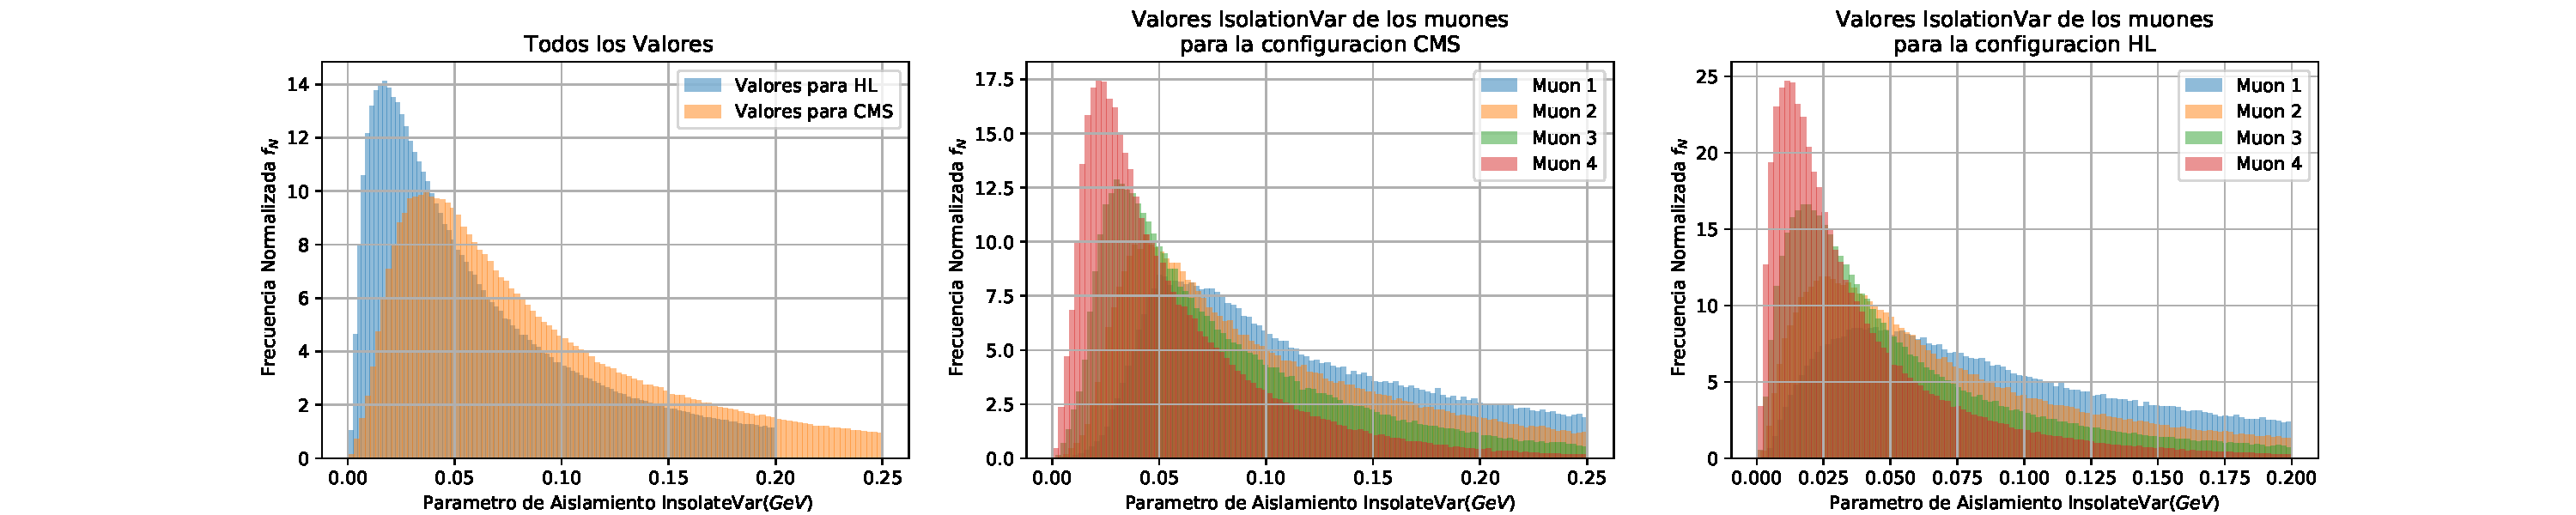
\includegraphics[width=.8\textwidth]{Simulacion/imagenes/Datos_IsolationVar_ALL.png}
\caption{Variación de las propiedades momento transversal y de la pseudorapidez de los muones en diferentes configuraciones del detector $k$ y ante variaciones del parámetro de generación $\vec{\alpha}$.}
\label{Comparacion}
\end{figure}

La caracterización de las propiedades de los muones $ \textsf{W}^{(\mu,k)} ({\textsf{x}_j})$, es parte importante de este estudio. Caracterizar las variaciones dependentes del parámetro de generación $\vec{\alpha}$ y los posibles cambios de estas propiedades resultado del cambio de la eficiencia de los detectores en sus diferentes configuraciones $k=\mathbf{R2}, \mathbf{HL}$ y compararlas con la teoría $k=\mathbf{True}$ es necesario para entender los cambios en la detección de los muones. 

Los valores generales del momento transversal mostrados en la Fig. \ref{Comparacion} y como varían sus distribuciones con los parámetros de generación se encontraron cambios en la morfología con los parámetros $m_{\gamma_D}$ y $m_{n_D}$, alternativamente una variación de la amplitud  en la escala de frecuencias con el parámetro de tiempo de vida del fotón oscuro $c\tau_{\gamma_D}$. Al comparar las distribuciones correspondientes a las diferentes configuraciones de los detectores se comprobó correctamente el aumento en la eficiencia de detección entre $\approx 6\%-14\%$ en la configuración de Alta Luminosidad para valores del momento de $P_T>10 ~GeV$. Además, a diferencia de la configuración Run-2, la configuración en Alta Luminosidad permitirá detectar muones de baja energía, información que será determinante con el aumento teórico del parámetro de masa del neutralino oscuro $m_{n_D}$, estos resultados con congruentes con los presentados en la Tabla \ref{Numero_de_Entradas}.

En la configuración  Run-2 existe un corte para valores de pseudorapidez de $|\eta|\lesssim 2.4$, correspondiendose al espectro donde se ubican el $\backsim 68\%$ de los muones. Por otro lado, en la configuración de Alta Luminosidad se obtienen partículas con $|\eta|\lesssim 4$, este nuevo dominio ocupa el rango correspondiente al $\backsim 96\%$ de las partículas generadas por la señal \MC. De lo anterior queda claro que la mejora esperada en el experimento \CMS, será determinante en la localización de las partículas provenientes de la teoría \MSSM\textbf{D}.



\subsection{Reconstruyendo el fotón oscuro}
Se está investigando el decaimiento $h \rightarrow 2n_1 \rightarrow 2n_D + 2\gamma_D \rightarrow 2n_D + 4\mu$ correspondiente al proceso \textbf{Dark-}\SUSY ~ o \MSSM\textbf{D} como se muestra en el diagrama de la Fig. \ref{fig:sketch_darksector}b. Se aplicarán 3 métodos diferentes para calcular la masa del fotón oscuro $\gamma_D$ correspondiente de este decaimiento. Estos métodos serán comparados y carcterizados para poder válidar sus ventajas y limitaciónes.

%, para poder reconstruir el fotón oscuro $\gamma_D$ se hará uso de los eventos característicos del estadístico $f^{(\mu, k)}_\textsf{e} (4;\vec{\alpha})$ ya que estos poseen la información necesaria para ello. Una de las problemáticas importantes a tener en cuenta en esta investigación es la reconstrucción del fotón oscuro con la mayor fiabilidad posible, para ello métodos que permitán disminuir los errores se hacen necesario. 


\subsubsection{Método $\mathbb{N}_\textsf{True}$}
%$\mathbb{N}_\textsf{True}$ 
%En los archivos $\textsf{*.root}$ 
Hace referencia a la comparación directa por eventos de la información obtenida por la  $\textsf{class GenParticle}$ relativa a las partículas generadas $k=\textsf{True}$ de nuestra señal \textbf{Dark-}\SUSY ~ y con la proporcionada por $\textsf{class Muon}$ se accede a la información resultado del proceso de hadronización y simulación del detector en la configuración elegida $k=\textsf{HL,R2}$. %Para reconocer el origen en la simulación de los muones reconstruidos por el detector, se hace necesario una comparación entre los muones generados y los detectados, sabido que estos poseen variaciones en sus propiedades resultado de los errores instrumentales. 
Para detectar el origen de las partículas que son reconstruidas por el detector se implementa un proceso iterativo de comparación entre los muones del detector y los generados, se consideran los mismos muones resultado de cumplir con dos requerimientos: 
\begin{itemize_f}
\item La diferencia en el momento transversal debe cumplir:
\begin{equation}
2\left|P_T^{(\mu_1)}-P_T^{(\mu_2)}\right|/\left[P_T^{(1)}+P_T^{(2)}\right] < .2
\end{equation} 
\item La distancia entre las partículas en el plano $\eta \times \phi$ sea mínima, o sea:
\begin{equation}
\min{\{\Delta R\}} = \sqrt{\left[\eta^{(\mu_1)} - \eta^{(\mu_2)}\right]^2 + \left[\phi^{(\mu_1)} - \phi^{(\mu_2)}\right]^2}
\end{equation}
\end{itemize_f} 
Dado que el origen de las partículas $k=\textsf{True}$ es determinado, esta comparación permite suponer con bajo porcentaje de error el origen de las partículas reconstruidas por el detector.

Entre las ventajas, esta la alta fiabilidad en los resultados y dicernimiento sobre el origen individual de cada muon. Entre sus desventajas, se encuentra, la imposibilidad de conocer los errores resultado de la comparación. %Su aplicación solo es posible ante datos simulados.

\subsubsection{Aplicando el método $\mathbb{N}_\textsf{True}$}
Se hace una caracterización general que reune en grupos todas las muestras simuladas con un valor del parámetro de masa del fotón oscuro específica $m_{\gamma_D}$. A estos grupos se les aplica el proceso de comparación siguiendo el método $\mathbb{N}_\textsf{True}$, y una vez identificada los di-muones reconstruidos se calcula masa invariante $m$, algunos ejemplos son gráficados en el Fig. \ref{mass_inv} y el valor de su moda $\widetilde{m}$ con los valores mínimos $\min{\{m\}}$ y máximos $\max{\{m\}}$. Además, bajo el análisis por eventos de los 2 di-muones para diferentes $k$ se calcula el valor correspondiente a la diferencia de la masa invariante $\Delta m\equiv|m_1-m_2|$ siempre que sea posible.


\begin{figure}[!h]
\centering
\includegraphics[width=.95\textwidth]{Cap4/imagenes/foton_mass.png}
%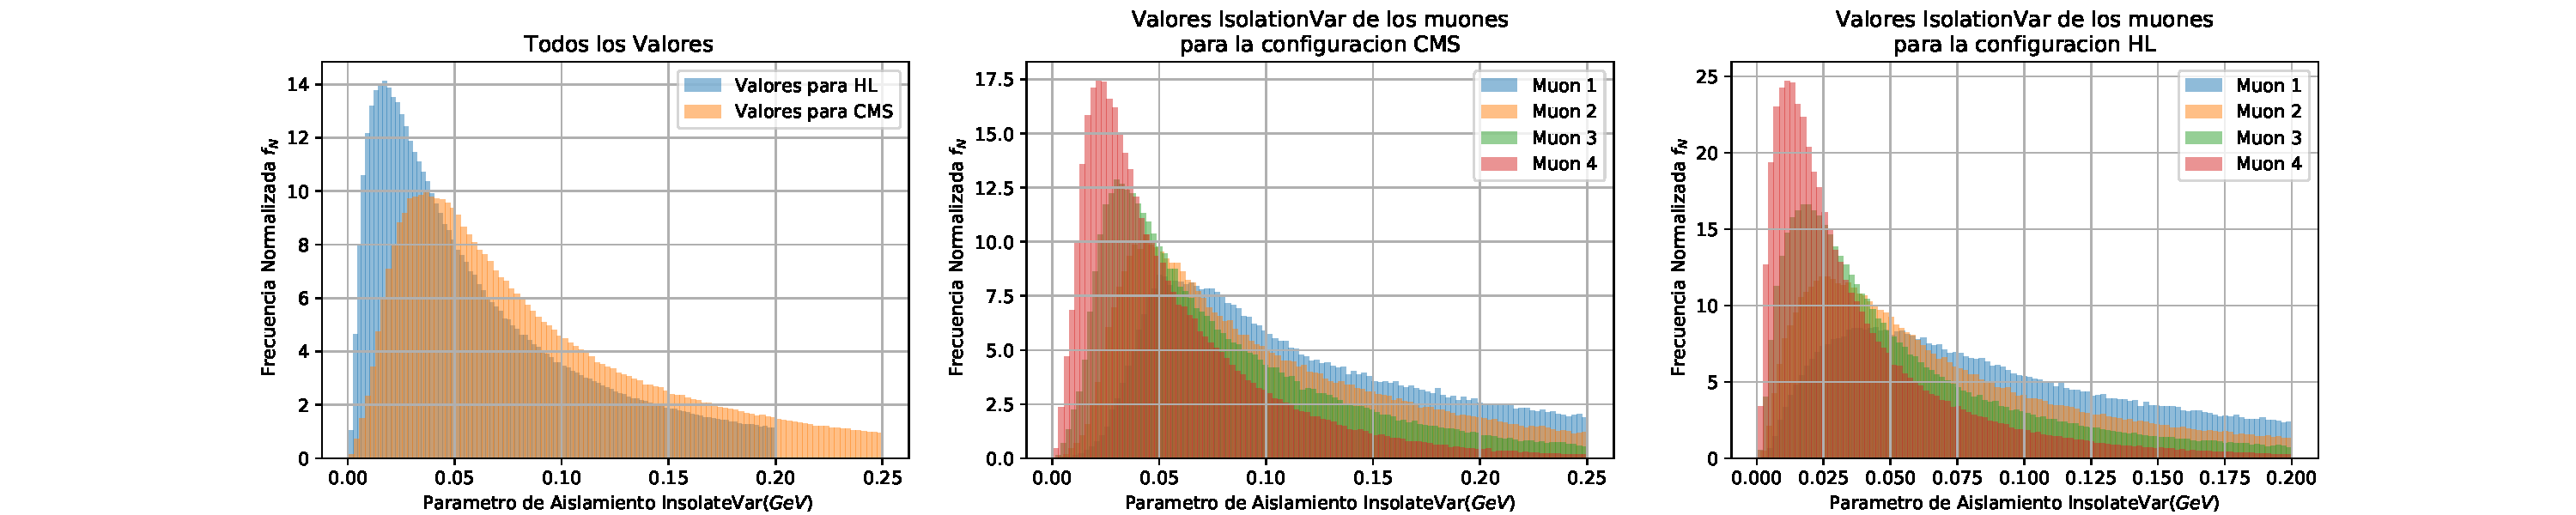
\includegraphics[width=.8\textwidth]{Simulacion/imagenes/Datos_IsolationVar_ALL.png}
\caption{Valores de masa invariante reconstruida de di-muones identificados con el método $\mathbb{N}_\textsf{True}$.}
\label{mass_inv}
%\includegraphics[width=.95\textwidth]{Simulacion/imagenes/foton_mass_diff.png}
%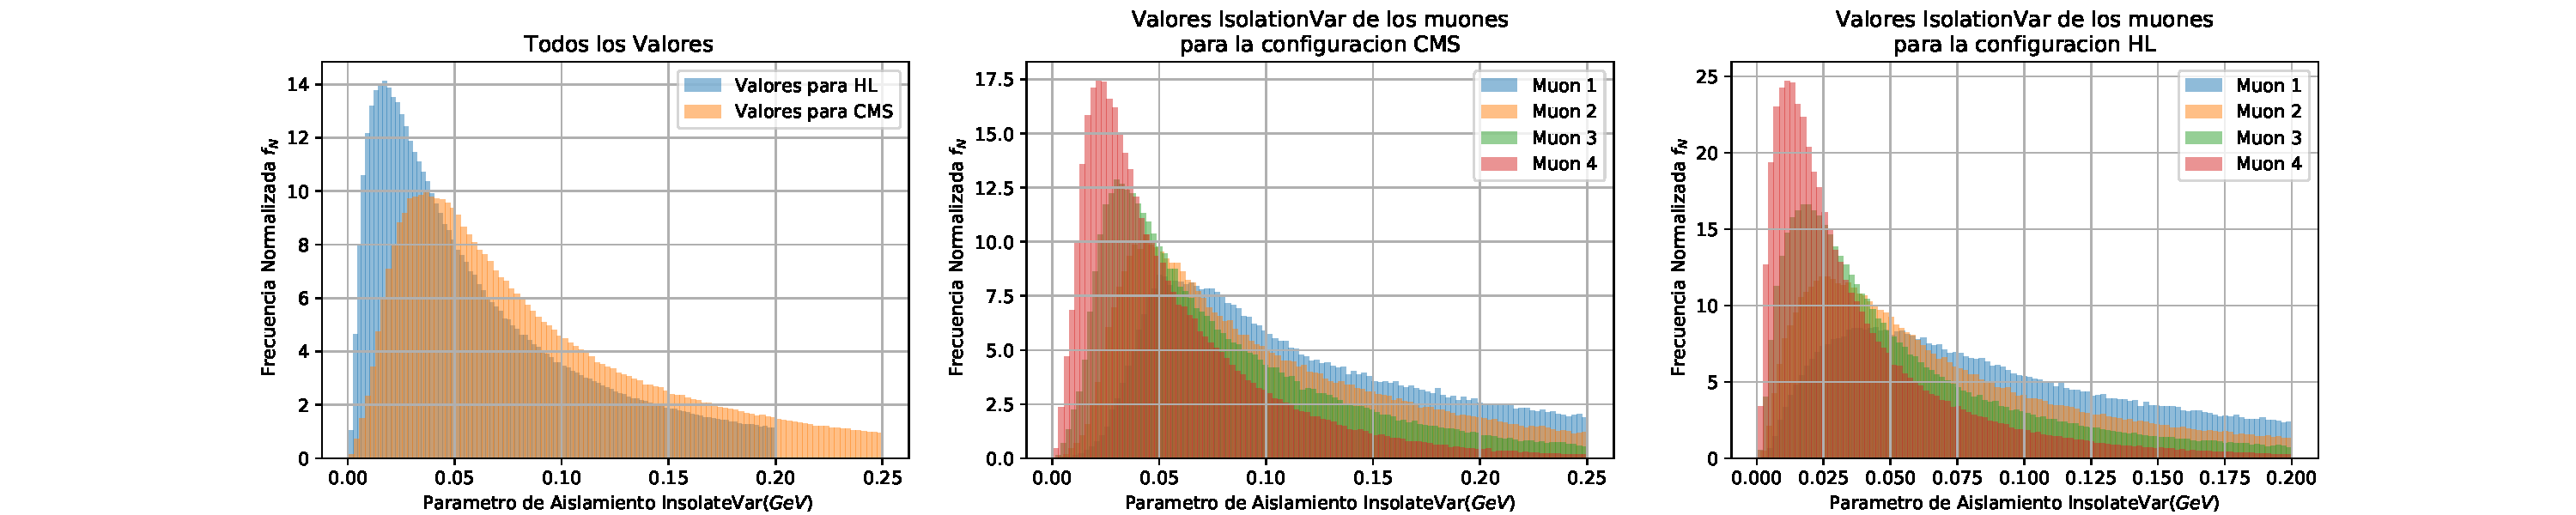
\includegraphics[width=.8\textwidth]{Simulacion/imagenes/Datos_IsolationVar_ALL.png}
%\caption{.}
%\label{mass_inv2}
\end{figure}-

%\begin{landscape}
\begin{table}[!t]
\centering
\footnotesize%small%scriptsize
\begin{tabular}{|c|cccccc|}
\toprule
Parámetro& \multicolumn{6}{c|}{Rango para el 95\% de los valores de $W_N^{(\gamma, ~ k)}$ }\\
$m_{\gamma_D}$ & \multicolumn{2}{c}{$\mathbf{k = True}$} & \multicolumn{2}{c}{$\mathbf{k = HL}$} & \multicolumn{2}{c|}{$\mathbf{k = R2}$}\\
(GeV)
& $\widetilde{m}^{~\max{\{m\}}}_{~\min{\{m\}}}$ & $\max{\{\Delta m\}}$
& $\widetilde{m}^{~\max{\{m\}}}_{~\min{\{m\}}}$ & $\max{\{\Delta m\}}$ 
& $\widetilde{m}^{~\max{\{m\}}}_{~\min{\{m\}}}$ & $\max{\{\Delta m\}}$ \\
\midrule
1 & $1.0070^{~1.1640}_{~0.9348}$ & 0.0649 & $0.9788^{~1.9138}_{~0.6466}$ & 1.2084 & $0.9972^{~2.3029}_{~0.6101}$ & 1.5625 \\ \midrule
2 & $1.9982^{~2.1223}_{~1.9065}$ & 0.1691 & $1.9884^{~2.7434}_{~1.5316}$ & 1.3099 & $1.9922^{3.0688}_{1.4182}$ & 1.6612\\ \midrule
3 & $2.9952^{~3.2272}_{~2.8510}$ & 0.3650 & $2.9905^{~3.6505}_{~2.5030}$ & 1.2725 & $2.9931^{~3.9416}_{~2.3468}$ & 1.6937\\ \midrule
4 & $4.0082^{~4.3908}_{~3.7929}$ & 0.5377 & $3.9909^{~4.5739}_{~3.4980}$ & 1.2403 & $3.9922^{~4.8446}_{~3.3280}$ & 1.6519\\ \midrule
5 & $5.0256^{~5.4876}_{~4.7461}$ & 0.6704 & $4.9916^{~5.5281}_{~4.5122}$ & 1.2048 & $4.9918^{~5.7624}_{~4.3372}$ & 1.5825 \\ \midrule
6 & $6.0373^{~6.5383}_{~5.6921}$ & 0.8072 & $5.9906^{~6.5903}_{~5.4170}$ & 1.3376 & $5.9897^{~6.8303}_{~5.2344}$ & 1.7378\\ \midrule
7 & $7.0193^{~7.6389}_{~6.6202}$ & 0.9784 & $6.9896^{~7.5784}_{~6.3953}$ & 1.3150 & $6.9897^{~7.7884}_{~6.2239}$ & 1.6676\\ \midrule
8 & $8.0253^{~8.7370}_{~7.5903}$ & 1.0795 & $7.9887^{~8.5680}_{~7.3765}$ & 1.3426 & $7.9858^{~8.7652}_{~7.2176}$ & 1.6717\\
\bottomrule 
\end{tabular}
\caption{Variación de estadísticos característicos para combinaciones de los términos del parámetro generación $\vec{\alpha}$ y los detectores $k$.}
\label{mass0}
\end{table}


%%\begin{landscape}
%\begin{table}[!t]
%\centering
%\scriptsize
%\begin{tabular}{|c|cccccc|}
%\toprule
%Parámetro& \multicolumn{6}{c|}{Rango para el 95\% de los valores de $W_N^{(\gamma, ~ k)}$ }\\
%$m_{\gamma_D}$ & \multicolumn{2}{c}{$\mathbf{k = True}$} & \multicolumn{2}{c}{$\mathbf{k = HL}$} & \multicolumn{2}{c|}{$\mathbf{k = R2}$}\\
%& $\widetilde{m} \pm \Delta m$ & $\max{|m_1 - m_2|}$ & $\widetilde{m} \pm \Delta m$ & $\max{|m_1 - m_2|}$ & $\widetilde{m} \pm \Delta m$ & $\max{|m_1 - m_2|}$\\
%\midrule
%1 & $1.0070^{1.1640}_{0.9348}$ & 0.0649 & $0.9788^{1.9138}_{0.6466}$ & 1.2084 & $0.9972^{2.3029}_{0.6101}$ & 1.5625 \\ \midrule
%2 & $1.9982^{2.1223}_{1.9065}$ & 0.1691 & $1.9884^{2.7434}_{1.5316}$ & 1.3099 & $1.9922^{3.0688}_{1.4182}$ & 1.6612\\ \midrule
%3 & $2.9952^{3.2272}_{2.8510}$ & 0.3650 & $2.9905^{3.6505}_{2.5030}$ & 1.2725 & $2.9931^{3.9416}_{2.3468}$ & 1.6937\\ \midrule
%4 & $4.0082^{4.3908}_{3.7929}$ & 0.5377 & $3.9909^{4.5739}_{3.4980}$ & 1.2403 & $3.9922^{4.8446}_{3.3280}$ & 1.6519\\ \midrule
%5 & $5.0256^{5.4876}_{4.7461}$ & 0.6704 & $4.9916^{5.5281}_{4.5122}$ & 1.2048 & $4.9918^{5.7624}_{4.3372}$ & 1.5825 \\ \midrule
%6 & $6.0373^{6.5383}_{5.6921}$ & 0.8072 & $5.9906^{6.5903}_{5.4170}$ & 1.3376 & $5.9897^{6.8303}_{5.2344}$ & 1.7378\\ \midrule
%7 & $7.0193^{7.6389}_{6.6202}$ & 0.9784 & $6.9896^{7.5784}_{6.3953}$ & 1.3150 & $6.9897^{7.7884}_{6.2239}$ & 1.6676\\ \midrule
%8 & $8.0253^{8.7370}_{7.5903}$ & 1.0795 & $7.9887^{8.5680}_{7.3765}$ & 1.3426 & $7.9858^{8.7652}_{7.2176}$ & 1.6717\\
%\bottomrule 
%\end{tabular}
%\caption{Variación de estadísticos característicos para combinaciones de los términos del parámetro generación $\vec{\alpha}$ y los detectores $k$.}
%%\label{mass0}
%\end{table}


\subsubsection{Método $\mathbb{N}_\textsf{RNA}$}
Una vez entrenado el identificador de di-muones específicado en la sección \ref{identificador_sec}, un proceso iteractivo es aplicado a todo emparejamiento posible entre los muones reconstruidos por el detector. La frecuencia del error al emparejar incorrectamente los elementos del di-muon es denotada como $\varepsilon_\textsf{RNA}$.

Entre las ventajas el hecho de que es un método general, este puede aplicarse sobre todos los eventos siempre que se tenga mínimo un muon de carga positiva y otro de carga negativa. Su fiabilidad es calculable al comparar los resultados obtenidos con el método $\mathbb{N}_\textsf{True}$. Entre sus desventajas esta el hecho de que solo puede dicernir sobre la pertenencia de los di-muones de un decaimiento \textbf{Dark-}\SUSY, la caracterización individual no es posible.


\subsubsection{Método $\mathbb{N}_\textsf{ite}$}
 
Se aplica un proceso iterativo sobre los eventos con un mínimo de 2 muones con carga positiva y 2 de carga negativa. Se emparejan todos los di-muones sin elemento en común de tal forma que la diferencia entre las masas invariantes $m$ resultantes sea mínima:
\begin{equation}
\Delta m_{\min} \equiv \min{\{\Delta m\}}  = \min{\{|m_1-m_2|\}}
\end{equation}
A este método se le puede anexar un corte que haga coherente la hipótesis de que los di-muones provienen de la misma partícula teórica, su aplicación implica que $\mathbb{N}_\textsf{ite} \Rightarrow \mathbb{N}_\textsf{ite}(\delta m)$, donde $\delta m > \Delta m_{\min}$ hace referencia al valor máximo admisible para la diferencia de masas invariantes. La frecuencia del error al emparejar incorrectamente los elementos del di-muon es denotada como $\varepsilon_\textsf{ite}$.

Entre las ventajas esta el hecho de que es un método general, su sencillez hace que sea fácilmente aplicable en cualquier investigación. Su fiabilidad es calculable al comparar los resultados obtenidos con el método $\mathbb{N}_\textsf{True}$. Entre sus desventajas esta el hecho de que solo puede recontruir pares de di-muones haciendo que la cantidad de 4 muones sea un requerimiento mínimo.















%En los archivos $\textsf{*.root}$ la clase $\textsf{GenParticle}$ posee toda la información relativa a las partículas generadas $k=\textsf{True}$ de nuestra señal \textbf{Dark-}\SUSY ~ y con la clase $\textsf{Muon}$ se accede a la información resultado del proceso de hadronización y simulación del detector en la configuración que fue elegida en el proceso de generación de los eventos $k=\textsf{HL,R2}$. Para reconocer el origen en la simulación de los muones reconstruidos por el detector, se hace necesario una comparación entre los muones generados y los detectados, sabido que estos poseen variaciones en sus propiedades resultado de los errores instrumentales. Para detectar su origen con cierta fiabilidad una proceso iterativo de comparación entre los muones del detector y los generados se hace necesario, este emparejamiento se realiza por evento, y cumple con los requisitos:
%\begin{enumerate}
%\item Encontrar muones en los que sus momentos transversales deben cumplir:
%\begin{equation}
%10~\textsf{GeV}~<|P_T^{(\mu,\textsf{True})}-P_T^{(\mu,\textsf{HL}/\textsf{R2})}|
%\end{equation}
%\item Emparejar muones en el que cumplan con la minimización del valor $\min(\Delta R)$, donde:
%\begin{equation}
%\Delta R = \sqrt{(\eta^{(\mu,\textsf{True})} - \eta^{(\mu,\textsf{HL}/\textsf{R2})})^2 + })
%\end{equation}
%\end{enumerate}











    
%%%%%%%%%%%%%%%%%%%%%%%%%%
%% Conclusiones %%
%%%%%%%%%%%%%%%%%%%%%%%%%%
\chapter*{Conclusiones}
Con el objetivo general de estudiar el decaimiento $h \rightarrow 2n_1 \rightarrow 2n_D + 2\gamma_D \rightarrow 2n_D + 4\mu$ correspondiente al modelo \textbf{Dark-}\SUSY, se creo un grupo de herramientas que facilitan el trabajo de simulación y análisis, entre estas están:
\begin{itemize_f}
\item Un generador programado en \textsf{python} que automatiza la simulación del decaimiento \textbf{Dark-}\SUSY~ utilizando \textsfSmall{ Madgraph5+pythia8+Delphes3} con alta adaptabilidad a los requerimientos del usuario.
\item Una clase basada en \textsfSmall{pyroot} para acceder a la información contenida en los archivos \textsfSmall{*.root}, permitiendo estos ser exportados en un formato \textbf{HDF5}.
\item Un método de selección de máximo de eventos $N_e$ basado en regresión polinomial y en \textbf{RNA}, permitiendo optimizar el proceso de generación para obtener la cantidad de eventos de interés con un mínimo de 4 muones que sea requerida por el estudio 
\item Un identificador de di-muones basado en redes neuronales utilizando la paquetería \textsf{keras} en \textsfSmall{python}.
\end{itemize_f}
Haciendo uso de estas herramientas se generó la base de datos utilizada en la exploración y análisis generales de esta investigación, donde se logra recrear correctamente el decaimiento a dos muones del fotón oscuro predicho por el modelo \textbf{Dark-}\SUSY~ bajo las configuraciones del detector \CMS ~ correspondiente a Run-2 y Alta Luminosidad, con diferentes condiciones en las propiedades dadas por el parámetro $\vec{\alpha}$. Al analizar los resultados, se observa una mejora en la probabilidad de reconstrucción del decaimiento como resultado de la actualización del detector \CMS~%en la obtención de información del decaimiento
fundamentado en aumentos de:
\begin{itemize_f}
\item El dominio de los valores de la pseudorapidez desde $|\eta|\lesssim 2.4$ hasta $|\eta|\lesssim 4$ permitiendo acceder desde un 68\% a un 98\% de total el espectro de la teoría.
\item El espectro del momento transversal desde un $P_T>10$ GeV a $P_T>2$ GeV.
\item La cantidad de eventos con potencial de reconstrucción total del decaimiento entre un $2.1 \lesssim f^{(\mu, \texttt{HL})}_\textsf{e} (4)/f^{(\mu, \texttt{R2})}_\textsf{e} (4) \lesssim 9$ veces.%, permitiendo aumentar las posibilidades de reconstruir completamente el decaimiento.
\item La cantidad de muones provenientes de la teoría y reconstruidos por los detectores entre un $1.3 \lesssim  A^{\mu}_n(\textsfSmall{HL})/A^{\mu}_n(\textsfSmall{R2}) \lesssim 2.8$ veces.
\end{itemize_f}
Se concluye que los valores de masa del neutralino oscuro $m_{n_D}$ son determinantes, junto con la masa del fotón oscuro $m_{\gamma_D}$ y su tiempo de vida $c\tau_{\gamma_D}$, en la reconstrucción de los muones provenientes de la teoría \textbf{Dark-}\SUSY.

Los análisis de los muones reconstruidos por el detector \CMS ~ permitieron analizar la capacidad total de reconstrucción correcta de los fotones oscuros como resultado del emparejamiento de los muones con carga eléctrica diferentes (di-muones) en las condiciones mostradas en la Tabla \ref{fotones_reconstruidos}, resultando en:
\begin{itemize_f}
\item Una reconstrucción entre un $0.024\lesssim  A_\textsf{True}^{\gamma_D} (\textsfSmall{R2})\lesssim 0.287$ del total de fotones predicho por la teoría en la configuración Run-2, mientras que, la configuración Alta Luminosidad reconstruye entre un $0.094\lesssim A_\textsf{True}^{\gamma_D} (\textsfSmall{HL})\lesssim 0.426$.
\item Una disminución en la dispersión de masas obtenidas entre un $\backsim 21\%-28\%$ para el 95\% de las masas obtenidas.

%Las distribuciones de masa invariante de los di-muones emparejados muestran 

\item Las diferencias de las masas invariantes reconstruidas en al menos el 95\% de decaimientos no excede los 2 GeV.  
\end{itemize_f}
Este análisis permitió validar dos métodos de identificación de di-muones sobre el conjunto de datos reconstruidos por el detector. El primero, implementando un identificador basado en redes neuronales $\mathbb{N}_\textsf{RNA}$ y permite la reconstrucción entre $92\% \lesssim \epsilon_{\textsf{RNA}} \lesssim 99\%$ del total de fotones oscuros que son posibles reconstruir con una precisión de $\textsf{acc}_\textsf{RNA}>0.93$. El segundo, se basa en un proceso de comparación de masas por eventos $\mathbb{N}_\textsf{ite}$, permitiendo reconstruir entre $3.5 \% \lesssim \epsilon_{\textsf{ite}}\lesssim 44\%$ de la capacidad total de reconstrucción con una precisión de $\textsf{acc}_\textsf{ite}>0.94$. 

Por lo tanto el método $\mathbb{N}_\textsf{RNA}$ es más eficiente en la reconstrucción de los di-muones que el método iterativo de comparación de masa, pero cada entrenamiento del identificador \textbf{RNA} hará que los resultados de su implementación sean diferentes dada la configuración y datos de entrenamiento a los que la investigación acceda. Por otro lado el método iterativo es mayormente más preciso, es simple en su ejecución y sus resultados pueden ser comparados e implementados de forma estándar en otros estudios semejantes.




%Dado lo cual, el objetivo de este proyecto es que se estudie, por medio de simulacion de \MC ~ el modelo teórico \textbf{Dark-}\SUSY, mediante la obtención teórica de las propiedades del fotón oscuro $\gamma_D$ en un entorno  simulado de los detectores que realizarían esta detección en dos  configuraciones ya conocidas del experimento \CMS, en la llamada Run-2 y en la  de Alta Luminosidad. En partícular en esta investigación se cumplen los objetivos partículares:\item Una clase basada en \textsfSmall{pyroot} para acceder a la información contenida en los archivos \textsfSmall{*.root}, permitiendo estos ser exportados los datos requeridos en un formato \textbf{HDF5}.


\addcontentsline{toc}{chapter}{Conclusiones}

    
    %\section{Muon efficiency parametrization}

%\section{Integration of Dark-SUSY model}

%\section{Delphes Simulation}

%\section{Muon system}

%\subsection{CMS detector}

%\subsection{Luminosity Era}

%\chapter{Simulation}

%\section{Parton Level and Hadronization}

%\section{Detector simulation}


%% Resultados y Analisis
%%\begin{textblock}{9}(2.5,-3)
%\begin{flushright}
%\setlength{\baselineskip}{15pt}
%\textblockrulecolour{white}
%~
%
%`` La discrepancia entre lo que se esperaba y lo que se ha observado ha aumentado a lo largo de los años, y nos estamos esforzando cada vez más por llenar el vacío
%''\\[.5cm]
%\textit{Jeremiah P. Ostriker}
%\end{flushright}
%\end{textblock}

En este capítulo se realiza una descripción del experimento \CMS, y una descripción del proceso de actualización de los detectores que lo componen. Se definen conceptos básicos correspondientes a la Física de Altas Energías experimental. Se introducen las herramientas personalizadas para el trabajo de simulación, análisis y caracterización en el área de partículas, entre estas se encuentras \ROOT, \textbf{Delphes}, \textbf{Pythia8} o \textbf{Madgraph}. Además, se introducen elementos comparativos para la caracterización del experimento en las configuración actual Run-2 y en la prevista en el futuro correspondiente a Alta Luminosidad.

%necesarios para el cumplimiento de los objetivos, estos serán descritos para su mejor comprensión en el proceso de simulación, caracterización y análisis de resultados. Además se resumirán los resultados que servirán de antecedentes para la investigación.






%\section{Algoritmo para el pareamiento de Muones}
Para la identificación de los procesos se implementa un algoritmo para la identificación de los decaimientos a dos muones y la identificacion de los di-muones en él:
\begin{figure}[ht!]
    \centering
    \includegraphics[width=0.84\textwidth]{Analisis_y_Resultados/imagenes/diagrama_pair.png}
    \caption{Diagrama de flujo para la identificación de los pares en los eventos a estudiar.}
    \label{fig:diagrama_pair}
\end{figure}


\section{Caracterizacion de la Señal}

%\begin{figure}[ht!]
%    \centering
    \includegraphics[width=0.84\textwidth]{Analisis_y_Resultados/imagenes/Cambio_de_D0_con_Card.png}
    
    \includegraphics[width=0.84\textwidth]{Analisis_y_Resultados/imagenes/Cambio_de_DZ_con_Card.png}
    
    \includegraphics[width=0.84\textwidth]{Analisis_y_Resultados/imagenes/Cambio_de_Eta_con_Card.png}
    
    \includegraphics[width=0.84\textwidth]{Analisis_y_Resultados/imagenes/Cambio_de_D0_con_Card.png}
    
    \includegraphics[width=0.84\textwidth]{Analisis_y_Resultados/imagenes/Cambio_de_IsolationVar_con_Card.png}
    
    \includegraphics[width=0.84\textwidth]{Analisis_y_Resultados/imagenes/Cambio_de_MassInv_con_Card.png}
    
    
    \includegraphics[width=0.84\textwidth]{Analisis_y_Resultados/imagenes/Cambio_de_Phi_con_Card.png}
    
    
    \includegraphics[width=0.84\textwidth]{Analisis_y_Resultados/imagenes/Cambio_de_PT_con_Card.png}
    
    





%\end{figure}




\begin{figure}[ht!]
    \centering
    \includegraphics[width=0.84\textwidth]{Analisis_y_Resultados/imagenes/evento_68.png}
    \caption{Representación esquematica de los pares generados en el evento 68 simulado: a) Reconstrucción con EVE; b) Identificación de elementos con C++.}
    \label{fig:diagrama_pair}
\end{figure}
\begin{figure}[ht!]
    \centering
    \includegraphics[width=0.84\textwidth]{Analisis_y_Resultados/imagenes/evento_68_info.png}
    \caption{Corte del informe del proceso de selección con C++ del evento 68.}
    \label{fig:diagrama_pair}
\end{figure}
\begin{figure}[ht!]
    \centering
    \includegraphics[width=0.84\textwidth]{Analisis_y_Resultados/imagenes/evento_7520.png}
    \caption{Representación esquematica de los pares generados en el evento 7520 simulado: a) Reconstrucción con EVE; b) Identificación de elementos con C++.}
    \label{fig:diagrama_pair}
\end{figure}
\begin{figure}[ht!]
    \centering
    \includegraphics[width=0.84\textwidth]{Analisis_y_Resultados/imagenes/evento_7520_info.png}
    \caption{Corte del informe del proceso de selección con C++ del evento 7520.}
    \label{fig:diagrama_pair}
\end{figure}

\begin{figure}[ht!]
    \centering
    \includegraphics[width=0.84\textwidth]{Analisis_y_Resultados/imagenes/mass.pdf}
    \caption{Masa invariante de los fotones pareados de nuestra se\~nal.}
    \label{fig:diagrama_pair}
\end{figure}

\begin{figure}[ht!]
    \centering
    \includegraphics[width=0.84\textwidth]{Analisis_y_Resultados/imagenes/MASS2.pdf}
    \caption{Masa invariante de los fotones pareados de nuestra se\~nal separados en los menores y los mayores.}
    \label{fig:diagrama_pair}
\end{figure}

\begin{figure}[ht!]
    \centering
    \includegraphics[width=0.84\textwidth]{Analisis_y_Resultados/imagenes/mulPT.pdf}
    \caption{Momento Angular ordenada para cada muon de nuestra se\~nal .}
    \label{fig:diagrama_pair}
\end{figure}



\section{Seleccion de Eventos}

La selecci\'on de eventos considera los cortes a distribuciones necesarios para maximizar la se\~nal y reducir lo mas posible la contribuci\'on 

\begin{table}[]
    \centering
    \begin{tabular}{|c|c|c|c|c|c|}
        \hline\hline
                                        & \multicolumn{5}{|c|}{N\'umero de Eventos HLLHC/CMS} \\

        Selecci\'on                     & c$\tau$=0mm   &  c$\tau$=5mm  & c$\tau$=10mm  & c$\tau$= 50mm & c$\tau$= 100mm\\ \hline
        Total                           & 10,000        & 10,000        & 10,000        & 10,000        & 10,000 \\ \hline
        (muones) $\mu >= 4$               & 1625 / 881    & 902/500       & 433/227       & 39/16         & 6/2 \\ \hline
        (di-muones)$\mu^+ \mu^->~= ~ 2$ & 1625 / 881    & 902/500       & 433/227       & 39/16         & 6/2 \\ \hline
        Isolation $<~ 2 GeV$            &               &               &               &               & \\ \hline\hline
    \end{tabular}
    \caption{Selecci\'on de eventos para muestras con masa de ``dark photon'' de $\gamma_{D}^{m}$ = 0.25 GeV}
    \label{tab:my_label}
\end{table}

%%%%%%%%%%%%%%%%%%%%%%%%%%
%% Anexos %%
%%%%%%%%%%%%%%%%%%%%%%%%%%
\appendix
%\chapter{Experimentos de Materia Oscura}\label{anexoA}
%Muchos fenónemos cosmólogicos han dado indicios de la existencia de materia oscura en sus diferentes composiciones teóricas, dado por lo cual un gran conjunto de experimentos han sido dedicados únicamente con la intención de obtener información pertinente en la comprensión de su composición y explicación de su comportamiento, existen dos métodos para realizar mediciones dimensionales:

% https://www.mpi-hd.mpg.de/hfm/CosmicRay/CosmicRaySites.html
\subsubsection{Forma directa}
Los métodos de detección directa intentan detectar las esporádicas interacciones que, a su paso por la Tierra, podrían experimentar
las partículas de materia oscura con un material adecuado y muy bien aislado del entorno.%Las mediciones directas utilizan instrumentos de medición para medir las propiedades físicas del objeto directamente, las mismas se pueden realizar en un amplio rango, especificado por la escala del instrumento de medición. 
Algunos experimentos de masa oscura son:

\begin{itemize_f}
\item[-] \href{https://en.wikipedia.org/wiki/Axion_Dark_Matter_Experiment}{ \textbf{ADMX} (\textbf{A}xion \textbf{D}ark \textbf{M}atter e\textbf{X}periment) :} 
\begin{itemize_f}
\item \textbf{Nombre:} \href{https://en.wikipedia.org/wiki/Axion_Dark_Matter_Experiment}{Experimento de Materia Oscura \Axion}
\item \textbf{Resumen:} Utiliza una cavidad de microondas resonante dentro de un gran imán superconductor para buscar \axiones~ de materia oscura fría en el halo local de materia oscura galáctica. 
\item \textbf{Pagina del proyecto :} \url{https://depts.washington.edu/admx/publications.shtml\#}
\end{itemize_f}




\item[-]\href{https://en.wikipedia.org/wiki/ANAIS}{\textbf{ANAIS} (\textbf{A}nnual modulation with \textbf{NAI} \textbf{S}cintillators) :} 
\begin{itemize_f}
\item \textbf{Nombre:} \href{https://en.wikipedia.org/wiki/ANAIS}{Modulación anual con NaI} \href{https://es.wikipedia.org/wiki/Centelleador}{Centelleador}.
\item \textbf{Resumen:} Busca la modulación anual de la señal con centelleadores de \href{https://es.wikipedia.org/wiki/Yoduro_de_sodio}{$NaI$} con el objetivo de detectar directamente  la Materia Oscura galáctica a través de su dispersión con los núcleos blanco de un cristal de NaI(Tl) radiopuro. Esta señal de Materia Oscura debería estar modulada anualmente debido al cambio de la velocidad relativa \WIMP-núcleo, consecuencia de la rotación de la Tierra alrededor del Sol.
\item \textbf{Pagina del proyecto :} \url{https://gifna.unizar.es/anais/}.
\end{itemize_f}

\item[-] \href{https://en.wikipedia.org/wiki/ArDM}{\textbf{ArDM} (\textbf{Ar}gon \textbf{D}ark \textbf{M}atter): }
\begin{itemize_f}
\item \textbf{Nombre:} \href{https://en.wikipedia.org/wiki/ArDM}{Materia Oscura en el Argón.}
\item \textbf{Resumen:} Busca medir y observando electrones libres de ionización y fotones de centelleo, que son producidos por la interación de su núcleo con los átomos vecinos y de esta forma relacionarla con la dispersión elástica de \WIMP ~ de los núcleos de argón líquido del que esta hecho el detector.
\item \textbf{Pagina del proyecto :} \url{https://wikimili.com/en/China_Jinping_Underground_Laboratory}.
\end{itemize_f}

%\item[-] \href{https://en.wikipedia.org/wiki/China_Dark_Matter_Experiment}{China Dark Matter Experiment (CDEX)}
%\begin{itemize_f}
%\item \textbf{Nombre:} 
%\item \textbf{Resumen:} 
%\item \textbf{Pagina del proyecto :} \url{}
%\end{itemize_f}

\item[-] \href{https://en.wikipedia.org/wiki/Cryogenic_Dark_Matter_Search}{\textbf{CDMS} (\textbf{C}ryogenic \textbf{D}ark \textbf{M}atter \textbf{S}earch)}
\begin{itemize_f}
\item \textbf{Nombre:} \href{https://en.wikipedia.org/wiki/Cryogenic_Dark_Matter_Search}{Buscando Materia Oscura Criogénica}
\item \textbf{Resumen:} Busca utilizando una serie de detectores de semiconductores a temperaturas de milikelvin encontrar los límites más sensibles en las interacciones de la materia oscura \WIMP~  con materiales terrestres y de esta manera detectar directamente la materia oscura. Constituye una serie de experimentos continuos: el \textbf{CDMS I}, \textbf{CDMS II}, el \textbf{SuperCDMS} y en la actualidad continúa con \textbf{SuperCDMS SNOLAB}.
\item \textbf{Pagina del proyecto :} \url{https://supercdms.slac.stanford.edu/}
\end{itemize_f}

%\item[-] \href{https://en.wikipedia.org/wiki/Cryogenic_Low-Energy_Astrophysics_with_Neon}{The Cryogenic Low-Energy Astrophysics with Noble liquids (CLEAN)}

%\item[-] \href{https://en.wikipedia.org/wiki/CoGeNT}{CoGeNT}
%\begin{itemize_f}
%\item \textbf{Nombre:} 
%\item \textbf{Resumen:} 
%\item \textbf{Pagina del proyecto :} \url{}
%\end{itemize_f}

%\item[-] \href{https://en.wikipedia.org/wiki/DAMA/LIBRA}{DAMA/LIBRA experiment}
%\begin{itemize_f}
%\item \textbf{Nombre:} Experimento \textbf{DAMA/LIBRA}
%\item \textbf{Resumen:} 
%\item \textbf{Pagina del proyecto :} \url{}
%\end{itemize_f}

\item[-] \href{https://en.wikipedia.org/wiki/DAMA/NaI}{DAMA/NaI experiment}
\begin{itemize_f}
\item \textbf{Nombre:} \href{https://en.wikipedia.org/wiki/DAMA/NaI}{Experimento DAMA/NaI}
\item \textbf{Resumen:} Características semejantes al experimento \href{https://en.wikipedia.org/wiki/ANAIS}{\textbf{ANAIS}} con mas de 7 años de datos de datos recopilados, fue continuado su estudio con el experimento \href{https://en.wikipedia.org/wiki/DAMA/LIBRA}{DAMA/LIBRA}.
\item \textbf{Pagina del proyecto :} \url{https://people.roma2.infn.it/~dama/web/home.html}
\end{itemize_f}

\item[-] \href{https://en.wikipedia.org/wiki/DarkSide}{DarkSide}
\begin{itemize_f}
\item \textbf{Nombre:} \href{https://en.wikipedia.org/wiki/DarkSide}{DarkSide}
\item \textbf{Resumen:} Busca con la construcción y operación de una serie de cámaras de proyección de tiempo o \href{https://en.wikipedia.org/wiki/Time_projection_chamber}{\textbf{TPC} (\textbf{T}ime \textbf{P}rojection \textbf{C}hamber)} de argón líquido para detectar \WIMPs. 
\item \textbf{Pagina del proyecto :} \url{http://darkside.lngs.infn.it/}
\end{itemize_f}

\item[-] \href{https://en.wikipedia.org/wiki/DEAP}{\textbf{DEAP} (\textbf{D}ark matter \textbf{E}xperiment using \textbf{A}rgon \textbf{P}ulse-shape discrimination)}
\begin{itemize_f}
\item \textbf{Nombre:} Experimento de materia oscura con discriminación de forma de pulso de argón
\item \textbf{Resumen:}) Busca discriminación de fondo basada en la característica forma de pulso de centelleo del argón permitiendo medir directamente \WIMP.
\item \textbf{Pagina del proyecto :} \url{http://deap3600.ca/}
\end{itemize_f}

%\item[-] \href{https://en.wikipedia.org/wiki/Monopole,_Astrophysics_and_Cosmic_Ray_Observatory}{MACRO (Monopole, Astrophysics and Cosmic Ray Observatory)}
%\begin{itemize_f}
%\item \textbf{Nombre:} 
%\item \textbf{Resumen:} 
%\item \textbf{Pagina del proyecto :} \url{}
%\end{itemize_f}
%
%\item[-] \href{https://en.wikipedia.org/wiki/PandaX}{PandaX (Particle and Astrophysical Xenon Detector)}
%\begin{itemize_f}
%\item \textbf{Nombre:} 
%\item \textbf{Resumen:} 
%\item \textbf{Pagina del proyecto :} \url{}
%\end{itemize_f}
%
%\item[-] \href{https://en.wikipedia.org/wiki/WIMP_Argon_Programme}{WIMP Argon Programme (WARP) }
%\begin{itemize_f}
%\item \textbf{Nombre:} 
%\item \textbf{Resumen:} 
%\item \textbf{Pagina del proyecto :} \url{}
%\end{itemize_f}
%
%\item[-] \href{https://en.wikipedia.org/wiki/XENON}{XENON}
%\begin{itemize_f}
%\item \textbf{Nombre:} 
%\item \textbf{Resumen:} 
%\item \textbf{Pagina del proyecto :} \url{}
%\end{itemize_f}
%
%\item[-] \href{https://en.wikipedia.org/wiki/ZEPLIN-III}{ZEPLIN-III dark matter experiment}
%\begin{itemize_f}
%\item \textbf{Nombre:} 
%\item \textbf{Resumen:} 
%\item \textbf{Pagina del proyecto :} \url{}
%\end{itemize_f}
%
%\item[-] \href{https://en.wikipedia.org/wiki/UK_Dark_Matter_Collaboration}{UK Dark Matter Collaboration (UKDMC)}
%\begin{itemize_f}
%\item \textbf{Nombre:} 
%\item \textbf{Resumen:} 
%\item \textbf{Pagina del proyecto :} \url{}
%\end{itemize_f}

\item[-] Otros experimentos : 
\begin{itemize_f}
\item \href{https://en.wikipedia.org/wiki/Monopole,_Astrophysics_and_Cosmic_Ray_Observatory}{\textbf{MACRO} (\textbf{M}onopole, \textbf{A}strophysics and \textbf{C}osmic \textbf{R}ay \textbf{O}bservatory)}, 

\textbf{Pagina del proyecto :} \url{https://hepwww.pp.rl.ac.uk/groups/ukdmc/ukdmc_old.html}

\item \href{https://en.wikipedia.org/wiki/PandaX}{PandaX (\textbf{P}article and Astrophysical \textbf{X}enon Detector)}, 

\textbf{Pagina del proyecto :} \url{https://pandax.sjtu.edu.cn/}

\item \href{https://en.wikipedia.org/wiki/WIMP_Argon_Programme}{\textbf{WARP} (\textbf{W}IMP \textbf{AR}gon \textbf{P}rogramme)}, 

\textbf{Pagina del proyecto :} \url{https://ztopics.com/WIMP\%20Argon\%20Programme/}

\item \href{https://en.wikipedia.org/wiki/XENON}{XENON}, 

\textbf{Pagina del proyecto :} \url{http://www.xenon1t.org/}

\item \href{https://en.wikipedia.org/wiki/ZEPLIN-III}{ZEPLIN-III dark matter experiment}, 

\textbf{Pagina del proyecto :} \url{https://zeplin.io/}

\item \href{https://en.wikipedia.org/wiki/UK_Dark_Matter_Collaboration}{\textbf{UKDMC} (\textbf{UK} \textbf{D}ark \textbf{M}atter \textbf{C}ollaboration)}, 

\textbf{Pagina del proyecto :} \url{https://hepwww.pp.rl.ac.uk/groups/ukdmc/ukdmc.html}
\end{itemize_f}
\end{itemize_f}


\subsubsection{Forma indirecta}
Otro mecanismo de investigación es cuando el valor de la propiedad física se obtiene a partir de lecturas directas de otras propiedades y de una expresión matemática que las relacione. Las medidas indirectas calculan el valor de la medida mediante una expresión matemática fundamentada por la teoría, previo cálculo de las magnitudes que intervienen en la expresión por medidas directas. Algunas investigaciones relacionadas con este mecanismo son: 

\begin{itemize_f}

\item[-] \href{https://en.wikipedia.org/wiki/Alpha_Magnetic_Spectrometer}{\textbf{AMS-02} (\textbf{A}lpha \textbf{M}agnetic \textbf{S}pectrometer)}
\begin{itemize_f}\label{AMS}
\item \textbf{Nombre:} Espectrómetro Magnético Alfa
\item \textbf{Resumen:} Busca con un detector localizado en Estación Espacial Internacional o \textbf{ISS} (\textbf{I}nternational \textbf{S}pace \textbf{S}tation) medir la antimateria en los rayos cósmicos, detectando picos en el flujo de positrones, antiprotones o rayos gamma pudiendo indicar la presencia de \neutralinos. El \textbf{AMS-01} es referido al prototipo de \textbf{AMS}, conteniendo este una versión simplificada del detector usado. Algunos de sus resultados se muestran en las referencias \cite{li_antiproton_2017,battiston_anti_2008}
\item \textbf{Pagina del proyecto :} \url{https://ams.nasa.gov/}
\end{itemize_f}

\item[-] \href{https://en.wikipedia.org/wiki/ANTARES_(telescope)}{\textbf{ANTARES} (\textbf{A}stronomy with a \textbf{N}eutrino \textbf{T}elescope and \textbf{A}byss environmental \textbf{RES}earch project)}
\begin{itemize_f}\label{antares}
\item \textbf{Nombre:} Astronomía con un Proyecto de Investigación Ambiental del Telescopio de Neutrinos y Abyss.
\item \textbf{Resumen:} Busca con sus tubos fotomultiplicadores detectar la radiación Cherenkov emitida cuando el muón pasa a través del agua, las técnicas de detección utilizadas consiguen en distinguir entre la señal de muones "que van hacia arriba", de neutrinos muónicos que interaccionan antes de llegar por debajo al detector y del alto flujo de muones procedentes de la atmósfera, con los datos y la alta resolución de estos pretende buscar indicaciones de materia oscura detectando el proceso de aniquilación del neutralino en el Sol. El proyecto \textbf{ANTARES} complementa el Observatorio de Neutrinos IceCube en la Antártida. Otros telescopios de neutrinos diseñados para su uso en el área cercana incluyen el telescopio griego \textbf{NESTOR} y el italiano \textbf{NEMO}. 

\item \textbf{Pagina del proyecto :} \url{https://antares.in2p3.fr/}

~~~~~~~~~~~~~~~~~~~~~~~~~~~~~~~~~\url{https://icecube.wisc.edu/}

~~~~~~~~~~~~~~~~~~~~~~~~~~~~~~~~~\url{https://cds.cern.ch/record/5841}

~~~~~~~~~~~~~~~~~~~~~~~~~~~~~~~~~\url{http://nemo.in2p3.fr/nemow3/index.html}
\end{itemize_f}

\item[-] \href{https://en.wikipedia.org/wiki/Calorimetric_Electron_Telescope}{\textbf{CALET} (\textbf{CAL}orimetric \textbf{E}lectron \textbf{T}elescope)}
\begin{itemize_f}\label{calet}
\item \textbf{Nombre:} Telescopio de electrones calorimétrico
\item \textbf{Resumen:} Busca realizar un seguimiento de la trayectoria de electrones, protones, núcleos y rayos gamma, mediante la medición de su dirección, carga y energía, para esto hace uso de un telescopio espacial de alta precisión.
\item \textbf{Pagina del proyecto :} \url{https://iss.jaxa.jp/en/kiboexp/ef/calet/}
\end{itemize_f}

%\item[-] \href{https://en.wikipedia.org/wiki/CERN_Axion_Solar_Telescope}{\textbf{CAST} (\textbf{C}ERN \textbf{A}xion \textbf{S}olar \textbf{T}elescope) }
%\begin{itemize_f}
%\item \textbf{Nombre:} 
%\item \textbf{Resumen:} es un experimento en física de astropartículas para buscar axiones que se originan en el sol. El experimento, realizado en el CERN en Suiza, comenzó en 2002 con la primera toma de datos a partir de mayo de 2003. La detección exitosa de los axiones solares constituiría un descubrimiento importante en la física de partículas y también abriría una nueva ventana sobre La astrofísica del núcleo solar.
%\item \textbf{Pagina del proyecto :} \url{}
%\end{itemize_f}

\item[-] \href{https://en.wikipedia.org/wiki/Dark_Matter_Particle_Explorer}{\textbf{DAMPE} (\textbf{DA}rk \textbf{M}atter \textbf{P}article \textbf{E}xplorer)}
\begin{itemize_f}
\item \textbf{Nombre:} Explorando Particulas de Materia Oscura
\item \textbf{Resumen:} Busca señal de descomposición indirecta de un hipotético candidato de materia oscura \WIMP~  mediante la detección rayos gamma de alta energía, electrones e iones de rayos cósmicos, para esto se hace uso de un telescopio espacial localizado en el satélite \textbf{CAS}.
\item \textbf{Pagina del proyecto :} \url{http://dpnc.unige.ch/dampe/}
\end{itemize_f}

\item[-] \href{https://en.wikipedia.org/wiki/Fermi_Gamma-ray_Space_Telescope}{\textbf{FGST} (\textbf{F}ermi \textbf{G}amma-ray \textbf{S}pace \textbf{T}elescope)}
\begin{itemize_f}\label{fermi}
\item \textbf{Nombre:} Telescopio Espacial de Area Grande de Rayos Gamma  
\item \textbf{Resumen:} Busca haciendo haciendo uso de un observatorio espacial muestras astronómicas de rayos gamma desde la órbita terrestre baja para para estudiar fenómenos astrofísicos y cosmológicos como núcleos galácticos activos, púlsares, otras fuentes de alta energía y materia oscura. Su instrumento principal es el Telescopio de Área Grande o \textbf{LAT} (\textbf{L}arge \textbf{A}rea \textbf{T}elescope), con el cual los astrónomos pretenden realizar un levantamiento de todo el cielo. %El proyecto es un experimento reconocido del CERN.
\item \textbf{Pagina del proyecto :} \url{https://glast.sites.stanford.edu/}
\end{itemize_f}

\item[-] \href{https://en.wikipedia.org/wiki/PAMELA_detector}{\textbf{PAMELA} (\textbf{P}ayload for \textbf{A}ntimatter \textbf{M}atter \textbf{E}xploration and \textbf{L}ight-nuclei \textbf{A}strophysics)}
\begin{itemize_f}\label{pamela}
\item \textbf{Nombre:} Exploración de la Materia-Antimateria y Astrofísica de los Núcleos de Luz.
\item \textbf{Resumen:} Busca estudiar y detectar rayos cósmicos, con un enfoque particular en su componente antimateria, en forma de positrones y antiprotones, además monitorea a largo plazo de la modulación solar de los rayos cósmicos, partículas energéticas del Sol, partículas de alta energía en la magnetosfera de la Tierra y electrones jovianos, con el objetivo de detectar evidencia de aniquilación de materia oscura.
\item \textbf{Pagina del proyecto :} \url{https://pamela.roma2.infn.it/}
\end{itemize_f}

\item[-] \href{https://stratocat.com.ar/fichas-e/1991/FSU-19910923.htm}{\textbf{MASS} (\textbf{M}atter \textbf{A}ntimatter \textbf{S}uperconducting \textbf{S}pectrometer)}
\begin{itemize_f}\label{mass}
\item \textbf{Nombre:} Espectrómetro Superconductor de Materia-Antimateria.
\item \textbf{Resumen:} Busca con la adaptación de la configuración básica de la Instalación de Imanes en Globo investigar partículas de alta energía usando un espectrómetro de imán superconductor, un dispositivo de tiempo de vuelo, un contador de gas cherenkov y un calorímetro de imagen de tubo streamer, de esta manera medir antiprotones en el rango de energías entre $4-20~GeV$ y positrones de aproximadamente $4-10~GeV$. Se utilizó la misma configuración del experimento \textbf{MASS-1} excepto por el sistema de seguimiento.

\item \textbf{Pagina del proyecto :} \url{https://stratocat.com.ar/fichas-e/1991/FSU-19910923.htm}
\end{itemize_f}

\item[-] \href{https://core.ac.uk/display/25103181}{\textbf{CAPRICE} (\textbf{C}osmic \textbf{A}nti\textbf{P}article \textbf{R}ing \textbf{I}maging \textbf{C}herenkov \textbf{E}xperiment)}
\begin{itemize_f}
\item \textbf{Nombre:} Experimento Cósmico de Imágenes de Anillo de Antipartículas de Cherenkov.
\item \textbf{Resumen:} Busca estudiar el flujo de rayos cósmicos sin demasiado fondo de partículas producidas atmosféricamente, esto es posible por el uso de un espectrómetro capaz de discriminar entre diferentes partículas. El proyecto se enfoca en estudiar los núcleos de antimateria, luz en los rayos cósmicos así como los muones en la atmósfera, específicamente mide el flujo de las antipartículas (antiprotones y positrones) por encima de aproximadamente $5~ GeV$ y relaciona los flujos con modelos que incluyen la producción exótica de antipartículas como partículas supersimétricas de materia oscura. %El flujo de muones se mide durante el descenso del globo a través de la atmósfera. Estas mediciones de flujo son importantes para los cálculos del flujo de neutrinos atmosféricos y, por lo tanto, para la interpretación de la anomalía del neutrino atmosférico.
\item \textbf{Pagina del proyecto :} \url{https://cds.cern.ch/record/5608}
\end{itemize_f}

\item[-] \href{https://ui.adsabs.harvard.edu/abs/1995psu..reptR....B/abstract}{\textbf{HEAT} (\textbf{H}igh-\textbf{E}nergy \textbf{A}ntimatter \textbf{T}elescope)}
\begin{itemize_f}
\item \textbf{Nombre:} Telescopio de Antimateria de Altas Energías
\item \textbf{Resumen:} Busca optimizadar la detección e identificación de electrones de rayos cósmicos y positrones a energías de aproximadamente $1~ GeV$ hasta $50~GeV$, mediante la implementación de un imán superconductor de dos bobinas y un hodoscopio de seguimiento de precisión, complementado con un sistema de tiempo de vuelo, un detector de radiación de transición y un contador de ducha electromagnético, de esta forma medir la diferencia en el tiempo entre la detección de una partícula ionizante en un tubo de deriva y un impulso generado por el disparador del experimento. Algunos de sus resultados se muestran en la referencia \cite{hooper_kaluza-klein_2004}.
\item \textbf{Pagina del proyecto :} \url{http://stratocat.com.ar/fichas-e/1994/FSU-19940503.htm}
\end{itemize_f}

\item[-] \href{https://en.wikipedia.org/wiki/Large_Hadron_Collider}{\textbf{LHC} (\textbf{L}arge \textbf{H}adron \textbf{C}ollider)}
\begin{itemize_f}\label{lhc}
\item \textbf{Nombre:} Gran Colisionador de Hadrones
\item \textbf{Resumen:} Ya que debido a que una partícula de materia oscura debería tener interacciones insignificantes con la materia visible normal, entonces estás interacciones pueden detectarse indirectamente como energía y momento faltantes que escapan de los detectores como resultado de las colisiones de haces de protones. Cualquier descubrimiento en las búsquedas de los colisionadores debe ser corroborado por resultados en los sectores de detección indirecta o directa en otros experimentos.
\item \textbf{Pagina del proyecto :} \href{https://home.cern/science/accelerators/large-hadron-collider}{\texttt{https://home.cern/science/accelerators/}}

~~~~~~~~~~~~~~~~~~~~~~~~~~~~~~~~~\href{https://home.cern/science/accelerators/large-hadron-collider}{ \texttt{large-hadron-collider}}. %aaaaaaaaaaaaaaa aaaaaaaaaaaaaaa \url{https://wikimili.com/en/China_Jinping_Underground_Laboratory}
\end{itemize_f}


\item[-] Otros experimentos : 
\begin{itemize_f}
\item[-] \href{https://en.wikipedia.org/wiki/Microlensing_Observations_in_Astrophysics}{\textbf{MOA} (\textbf{M}icrolensing \textbf{O}bservations in \textbf{A}strophysics) }

\textbf{Pagina del proyecto :} \url{http://www.tekapotourism.co.nz/info/mt_john.html}

\item[-] \href{https://en.wikipedia.org/wiki/VERITAS}{\textbf{VERITAS} (\textbf{V}ery \textbf{E}nergetic \textbf{R}adiation \textbf{I}maging \textbf{T}elescope \textbf{A}rray \textbf{S}ystem)}

\textbf{Pagina del proyecto :} \url{https://veritas.sao.arizona.edu/}
\end{itemize_f}


\end{itemize_f}

%\subsubsection{Generanción de materia oscura por coalición}



%\chapter{Compilación de la sección transversal hadrónica}\label{anexoA}
%%\begin{landscape}
\begin{table}[!h]
\centering
\footnotesize
\begin{tabular}{|cccc|}
\toprule
$\sqrt{s}$ & Valores de $R$ & Experimento & Enlace\\ \midrule
$1841.0\pm 2$ 	& $2.226 \pm 0.139\pm 0.158$ &  \textbf{KEDR} & \cite{RRKerd}\\%*
$1937.0\pm 2$ 	& $2.141 \pm 0.081\pm 0.073$ &  \textbf{KEDR} & \cite{RRKerd}\\%*
$2037.3\pm 2$ 	& $2.238 \pm 0.068\pm 0.072$ &  \textbf{KEDR} & \cite{RRKerd}\\%*
$2135.7\pm 2$ 	& $2.275 \pm 0.072\pm 0.055$ &  \textbf{KEDR} & \cite{RRKerd}\\%*
$2239.2\pm 2$ 	& $2.208 \pm 0.069\pm 0.053$ &  \textbf{KEDR} & \cite{RRKerd}\\%*
$2339.5\pm 2$ 	& $2.194 \pm 0.064\pm 0.048$ &  \textbf{KEDR} & \cite{RRKerd}\\%*
$2444.1\pm 2$ 	& $2.175 \pm 0.067\pm 0.048$ &  \textbf{KEDR} & \cite{RRKerd}\\%*
$2542.6\pm 2$ 	& $2.222 \pm 0.070\pm 0.047$ &  \textbf{KEDR} & \cite{RRKerd}\\%*
$2644.8\pm 2$ 	& $2.220 \pm 0.069\pm 0.049$ &  \textbf{KEDR} & \cite{RRKerd}\\%*
$2744.6\pm 2$ 	& $2.269 \pm 0.065\pm 0.050$ &  \textbf{KEDR} & \cite{RRKerd}\\%*
$2849.7\pm 2$ 	& $2.223 \pm 0.065\pm 0.047$ &  \textbf{KEDR} & \cite{RRKerd}\\%*
$2948.9\pm 2$ 	& $2.234 \pm 0.064\pm 0.051$ &  \textbf{KEDR} & \cite{RRKerd}\\%*
$3048.1\pm 2$ 	& $2.278 \pm 0.075\pm 0.048$ &  \textbf{KEDR} & \cite{RRKerd}\\%*
$3076.7\pm 2$ 	& $2.188 \pm 0.056\pm 0.042$ &  \textbf{KEDR} & \cite{RRKerd}\\%*

$3119.6\pm 0.4$	& $2.235 \pm 0.042\pm 0.049$ &  \textbf{KEDR} & \cite{RRKerd}\\
$3119.9\pm 0.4$	& $2.237 \pm 0.089\pm 0.066$ &  \textbf{KEDR} & \cite{RRKerd2}\\
$3222.5\pm 0.8$ & $2.195 \pm 0.040\pm 0.035$ &  \textbf{KEDR} & \cite{RRKerd}\\
$3223.0\pm 0.6$ & $2.173 \pm 0.057\pm 0.045$ &  \textbf{KEDR} & \cite{RRKerd2}\\
$3314.7\pm 0.6$	& $2.219 \pm 0.035\pm 0.035$ &  \textbf{KEDR} & \cite{RRKerd}\\
$3314.7\pm 0.7$	& $2.200 \pm 0.056\pm 0.043$ &  \textbf{KEDR} & \cite{RRKerd2}\\
$3418.3\pm 0.2$ & $2.168 \pm 0.050\pm 0.042$ &  \textbf{KEDR} & \cite{RRKerd2}\\
$3418.3\pm 0.3$ & $2.185 \pm 0.032\pm 0.035$ &  \textbf{KEDR} & \cite{RRKerd}\\
$3499.6\pm 0.4$ & $2.224 \pm 0.054\pm 0.040$ &  \textbf{KEDR} & \cite{RRKerd}\\
$3520.8\pm 0.4$	& $2.201 \pm 0.050\pm 0.044$ &  \textbf{KEDR} & \cite{RRKerd}\\
$3618.2\pm 1.0$ & $2.218 \pm 0.038\pm 0.035$ &  \textbf{KEDR} & \cite{RRKerd}\\
$3618.2\pm 1.0$ & $2.207 \pm 0.059\pm 0.044$ &  \textbf{KEDR} & \cite{RRKerd2}\\
$3719.4\pm 0.7$ & $2.228 \pm 0.039\pm 0.042$ &  \textbf{KEDR} & \cite{RRKerd}\\
$3719.4\pm 0.7$ & $2.187 \pm 0.068\pm 0.060$ &  \textbf{KEDR} & \cite{RRKerd2}\\

$8400.0\pm 2000.0$ & $3.370 \pm 0.060\pm 0.230$ &  \textbf{ARGUS} & \cite{R8}\\%*
$8795.0\pm 3090.0$ & $3.580 \pm 0.020\pm 0.140$ &  \textbf{LENA} & \cite{R8}\\%*
\bottomrule 
\end{tabular}
\caption{.}
\label{rvalues}
\end{table}
%\end{landscape} 
%\chapter{Name of Appendix B}
%\label{whatever}
%\input{appendixB} % filename in curly brackets

\clearpage
\phantomsection

\bibliographystyle{UNAMThesis}
%\bibliographystyle{abbrv}
%\bibliographystyle{APA}
\bibliography{ParticleUnison}
%\bibliography{references}
\addcontentsline{toc}{chapter}{Referencias}
\end{document}













